\documentclass[11pt,a4paper]{article}

\usepackage[T1]{fontenc}
\usepackage[utf8]{inputenc}
\usepackage[french]{babel}
\usepackage{amsmath,amssymb}
\usepackage[margin=2.3cm]{geometry}
\usepackage{booktabs}
\usepackage{graphicx}
\usepackage{array}
\usepackage{textcomp}
\usepackage{enumitem}
\usepackage{float}
\usepackage{longtable}
\usepackage{tikz}
\usetikzlibrary{arrows.meta,positioning,patterns}
\usepackage[colorlinks=true,linkcolor=blue,citecolor=blue]{hyperref}

\newsavebox{\implbox}
\newenvironment{implication}%
  {\par\medskip\begin{lrbox}{\implbox}\begin{minipage}{0.95\textwidth}%
   \textbf{Lien avec la pratique.}\itshape\ }%
  {\end{minipage}\end{lrbox}\noindent\fbox{\usebox{\implbox}}\par\medskip}

% Environnements propres à l'annexe (guide de mise en œuvre)
\newsavebox{\attbox}
\newenvironment{attention}%
  {\par\medskip\begin{lrbox}{\attbox}\begin{minipage}{0.95\textwidth}%
   \textbf{À retenir.}\itshape\ }%
  {\end{minipage}\end{lrbox}\noindent\fbox{\usebox{\attbox}}\par\medskip}

\newsavebox{\critbox}
\newenvironment{critere}%
  {\par\medskip\begin{lrbox}{\critbox}\begin{minipage}{0.95\textwidth}%
   \textbf{Critère de réussite.}\ }%
  {\end{minipage}\end{lrbox}\noindent\fbox{\usebox{\critbox}}\par\medskip}

\newcommand{\eps}{\varepsilon_r}
\newcommand{\ee}{\mathrm{e}}
\newcommand{\jj}{\mathrm{j}}
\newcommand{\nvec}{\hat{\mathbf{n}}}

\graphicspath{{figures/}{diag_bande/}}

\title{\bfseries Cartographie sans contact de l'interface cartilage--os\\
       par radar à balayage de fréquence\\[2mm]
       \large Théorie, limites fondamentales et faisabilité du dixième de
       millimètre\\ dans le contexte de l'arthroplastie totale de genou}
\author{Notes de travail --- projet LiteVNA}
\date{\today}

\begin{document}
\maketitle

\begin{abstract}
\noindent
On cherche à reconstruire, dans le repère du robot, la surface de l'interface
cartilage--os d'un genou ouvert pendant une arthroplastie totale (TKA), à partir
de mesures radar sans contact effectuées par une sonde portée par un bras à
six degrés de liberté. La surface externe du cartilage est déjà connue par un
relevé optique tridimensionnel ; l'épaisseur recherchée vaut de $0$ à $5$~mm et
la précision visée est de l'ordre de $0{,}1$~mm. Ces notes établissent les
limites fondamentales de la mesure, montrent pourquoi la limite de résolution
classique ne s'applique pas au problème posé, et concluent que l'objectif est
atteignable \emph{à condition} de maîtriser la permittivité du cartilage à
environ $4\,\%$ et d'éliminer la dérive mécanique du montage. Les valeurs
numériques proviennent de mesures effectuées sur notre propre banc.

\medskip\noindent
Le cahier des charges complet est confronté à ses limites physiques au
tableau~\ref{tab:cdc_revise}. Deux conclusions s'en dégagent : la précision en
épaisseur est acquise et ne dépend plus que de la connaissance de $\eps$ ;
en revanche la \emph{résolution latérale} est bornée par la diffraction à
$\lambda/4 = 11{,}9$~mm, et c'est le seul poste qui distingue le LiteVNA d'un
instrument à $15$~GHz. Il est montré en particulier qu'élargir la bande au-delà
de $15$~GHz n'apporte rien --- l'absorption diélectrique de l'eau y annule toute
information --- et que la distance antenne--objet n'a pas besoin d'être connue,
la mesure étant auto-référencée.
\end{abstract}

\tableofcontents
\bigskip\hrule\bigskip

%=======================================================================
\section{L'application}
%=======================================================================

\subsection{Contexte clinique et dispositif}

Lors d'une arthroplastie totale de genou, le champ opératoire expose
directement le cartilage articulaire. Un système optique reconstruit la
\emph{surface externe} du cartilage sous forme d'un maillage tridimensionnel.
Ce qui manque au chirurgien est la \emph{surface interne} : l'interface entre le
cartilage et l'os sous-chondral, qui détermine la coupe osseuse.

Une sonde radar, portée par un robot à six degrés de liberté, est déplacée
au-dessus de la surface. À chaque pose elle mesure le coefficient de réflexion
complexe $S_{11}(f)$ sur la bande $1{,}4$--$6{,}3$~GHz, dont on extrait
l'épaisseur locale $d$ du cartilage.

\begin{center}
\begin{tikzpicture}[scale=1.15]
  % Surface externe du cartilage
  \draw[very thick, blue!70!black]
     plot[smooth, tension=0.8] coordinates {(0,0)(1.2,0.55)(2.6,0.85)(4,0.7)(5.2,0.25)(6,-0.1)};
  \node[blue!70!black, right] at (6.05,-0.1) {\small surface externe (optique)};
  % Interface cartilage-os
  \draw[very thick, orange!80!black]
     plot[smooth, tension=0.8] coordinates {(0,-0.45)(1.2,0.05)(2.6,0.30)(4,0.22)(5.2,-0.15)(6,-0.5)};
  \node[orange!80!black, right] at (6.05,-0.5) {\small interface cartilage--os (\textbf{cherchée})};
  % Os
  \fill[pattern=north east lines, pattern color=gray!60, opacity=0.5]
     plot[smooth, tension=0.8] coordinates {(0,-0.45)(1.2,0.05)(2.6,0.30)(4,0.22)(5.2,-0.15)(6,-0.5)}
     -- (6,-1.4) -- (0,-1.4) -- cycle;
  \node[gray!50!black] at (3,-1.0) {os sous-chondral};
  % Antenne
  \draw[very thick, fill=gray!25] (2.05,2.05) rectangle (3.15,2.45);
  \node at (2.6,2.25) {\small antenne};
  \draw[-{Latex[length=2mm]}, very thick, red] (2.6,2.05) -- (2.6,0.9);
  \node[red, right] at (2.63,1.5) {\small $\nvec$ (normale)};
  % Cotes
  \draw[<->, thick] (3.6,0.76) -- (3.6,0.25);
  \node[right] at (3.62,0.5) {\small $d$};
  \draw[<->, thick] (1.5,2.05) -- (1.5,0.62);
  \node[left] at (1.48,1.35) {\small $h$ (standoff)};
  % Points
  \fill[blue!70!black] (2.6,0.85) circle (1.6pt);
  \node[above left] at (2.55,0.87) {\small $\mathbf{P}_{\text{ext}}$};
  \fill[orange!80!black] (2.6,0.30) circle (1.6pt);
  \node[below left] at (2.55,0.28) {\small $\mathbf{P}_{\text{int}}$};
  % Balayage
  \draw[-{Latex[length=2mm]}, thick, gray] (3.35,2.62) -- (4.5,2.62);
  \draw[-{Latex[length=2mm]}, thick, gray] (1.85,2.62) -- (0.7,2.62);
  \node[gray] at (2.6,2.75) {\small balayage robot 6 axes};
\end{tikzpicture}
\end{center}

\subsection{L'équation de reconstruction}

Le robot étant supposé sans erreur de positionnement, et la surface externe
étant connue avec sa normale $\nvec$ en chaque point, la reconstruction est
immédiate :

\begin{equation}
\boxed{\;\mathbf{P}_{\text{int}} \;=\; \mathbf{P}_{\text{ext}}
        \;-\; d\,\nvec\;}
\label{eq:reconstruction}
\end{equation}

L'erreur sur la surface interne se réduit donc à l'erreur sur $d$, projetée le
long de la normale. \emph{Tout le problème se ramène à estimer un scalaire.}

\subsection{Cahier des charges}
\label{sec:cdc}

\begin{table}[h]
\centering
\begin{tabular}{ll}
\toprule
Épaisseur à mesurer & $d \in [0\,;\,5]$~mm \\
Précision visée & $\sigma_d \simeq 0{,}1$~mm \\
Distance antenne--objet & $20$ à $500$~mm \\
Résolution latérale visée & $5$~mm \\
Vitesse des objets & nulle (scène statique) \\
Contact & \textbf{aucun} : ni os, ni cartilage, ni peau \\
Porteur & robot 6 axes, erreur de positionnement supposée nulle \\
Bande & $1{,}4$--$6{,}3$~GHz ($B = 4{,}9$~GHz), $N = 101$ points \\
Milieu & cartilage $\eps \simeq 40$--$45$, $\sigma \simeq 1{,}7$~S/m ;
         os $\eps \simeq 10$--$12$ \\
\bottomrule
\end{tabular}
\end{table}

\noindent
Ces exigences ne sont pas toutes compatibles entre elles ni avec la physique.
Le tableau~\ref{tab:cdc_revise} (\S\ref{sec:synthese}) confronte chacune d'elles
à sa limite fondamentale et donne la valeur réellement atteignable ; les
sections intermédiaires en établissent le détail. Deux résultats méritent d'être
annoncés dès maintenant, car ils orientent tout le reste :

\begin{itemize}
\item la \textbf{résolution latérale} est le seul poste qui disqualifie le
      LiteVNA. Elle est bornée par la diffraction à $\lambda/4 = 11{,}9$~mm à
      $6{,}3$~GHz, quelle que soit l'ouverture (\S\ref{sec:lateral}) ;
\item la \textbf{connaissance de $\eps$} est le seul poste qui décide de la
      précision. La seule dispersion de littérature sur le cartilage
      ($40$ à $45$) produit déjà $0{,}147$~mm d'erreur à $5$~mm d'épaisseur,
      soit davantage que la cible (\S\ref{sec:milieux}).
\end{itemize}

%=======================================================================
\section{Le point de départ : la recherche de deux pics}
\label{sec:deuxpics}
%=======================================================================

Avant d'aborder la théorie, il faut décrire ce qui a déjà été construit, ce que
cette approche vaut, et pourquoi elle doit évoluer.

\subsection{La chaîne actuelle}

Le programme existant met en \oe uvre une chaîne de traitement classique de
radar à balayage de fréquence, en temps réel :

\begin{center}
\begin{tikzpicture}[
   node distance=3.5mm,
   bloc/.style={draw, thick, rounded corners=1.5pt, align=center,
                inner sep=3pt, font=\footnotesize, minimum height=9mm},
   fl/.style={-{Latex[length=1.8mm]}, thick}]
  \node[bloc, fill=blue!8]   (a) {$S_{11}(f)$\\LiteVNA};
  \node[bloc, right=of a, fill=blue!8]   (b) {tare\\$-\,S_{11}^{\text{vide}}$};
  \node[bloc, right=of b, fill=blue!8]   (c) {fenêtre\\de Hann};
  \node[bloc, right=of c, fill=blue!8]   (d) {IFFT\\zéro-pad. $\times 8$};
  \node[bloc, right=of d, fill=orange!14](e) {module\\$|\cdot|$};
  \node[bloc, below=6mm of e, fill=orange!14] (f) {\texttt{find\_peaks}\\prominence};
  \node[bloc, left=of f, fill=orange!14] (g) {suivi EMA\\porte + coasting};
  \node[bloc, left=of g, fill=green!12]  (h) {$d = \dfrac{\Delta r}{\sqrt{\eps}}$};
  \foreach \x/\y in {a/b,b/c,c/d,d/e} {\draw[fl] (\x) -- (\y);}
  \draw[fl] (e) -- (f);
  \draw[fl] (f) -- (g);
  \draw[fl] (g) -- (h);
  \node[font=\scriptsize, above=1mm of c] {information complexe conservée};
  \node[font=\scriptsize, red!70!black, below=1mm of e]
       {\textbf{la phase est jetée ici}};
\end{tikzpicture}
\end{center}

L'épaisseur est obtenue comme la \emph{différence} des positions de deux pics,
divisée par $\sqrt{\eps}$ que règle un curseur. Le suivi (lissage exponentiel,
porte de rejet, mémoire de quelques trames) stabilise l'affichage lorsqu'un pic
disparaît momentanément.

\subsection{Ce que cette approche a pour elle}

\begin{enumerate}
\item \textbf{Elle est différentielle.} L'épaisseur étant une différence de deux
      positions, tout retard systématique --- longueur de câble, plan de
      référence, absence de calibration SOL --- se soustrait exactement. C'est
      la raison profonde pour laquelle elle donne des résultats utilisables sans
      calibration vectorielle.
\item \textbf{Elle ne suppose aucun modèle.} Aucune connaissance préalable du
      matériau n'est requise en dehors de $\eps$ ; elle fonctionne sur la
      gélatine, le plexiglas, un livre, indifféremment.
\item \textbf{Elle est directement lisible.} L'opérateur voit le profil, les
      pics, la fenêtre de détection. C'est un instrument de réglage et de
      diagnostic irremplaçable : viser, vérifier la tare, contrôler l'échelle
      des distances, détecter un câble qui bouge.
\item \textbf{Elle est rapide} et tourne en temps réel.
\item \textbf{Elle est juste dans son domaine de validité}, c'est-à-dire
      au-delà de $53$~mm dans l'air, soit $8{,}4$~mm dans le cartilage.
\end{enumerate}

\subsection{Ce qui la disqualifie pour le cartilage}

\begin{enumerate}
\item \textbf{Obstacle fondamental.} Elle demande deux pics \emph{séparés}. Or
      la résolution vaut $8{,}4$~mm dans le cartilage (éq.~\ref{eq:rayleigh}) et
      la cible en fait $0$ à $5$. La méthode est structurellement hors domaine, et
      aucun réglage ne l'y ramènera.
\item \textbf{Elle jette la phase.} Le passage au module au moment de la
      détection de pics élimine la moitié de l'information mesurée --- celle-là
      même sur laquelle repose toute la suite du document.
\item \textbf{La fenêtre coûte cher.} L'apodisation de Hann élargit le lobe
      principal d'un facteur $1{,}7$ : $30{,}6$~mm théoriques deviennent
      $53$~mm effectifs.
\item \textbf{Elle n'exploite rien de ce que l'on sait.} Surface externe
      connue, normale connue, ordre du modèle connu, permittivité connue : rien
      de tout cela n'entre dans le calcul.
\item \textbf{Elle ne fournit pas de barre d'erreur.} Un pic est détecté ou non,
      sans indication de confiance.
\end{enumerate}

\subsection{Le verdict, chiffré}

Simulation Monte-Carlo sur la chaîne exacte, second écho à $-10$~dB,
$300$~tirages :

\begin{table}[h]
\centering
\begin{tabular}{lccc}
\toprule
Épaisseur de cartilage & $3$~mm & $2$~mm & $1$~mm \\
\midrule
Deux pics (chaîne actuelle) & erreur $7{,}3$~mm & échec & échec \\
Inversion sur modèle, montage stabilisé
   & $0{,}003$~mm & $0{,}007$~mm & $0{,}006$~mm \\
\bottomrule
\end{tabular}
\end{table}

\noindent
« Échec » signifie que la chaîne ne détecte même pas deux pics. À $3$~mm elle
en détecte deux, mais se trompe de $7{,}3$~mm : elle mesure la largeur du lobe
d'apodisation, pas l'épaisseur.

\subsection{Recommandation}

\begin{center}
\fbox{\begin{minipage}{0.94\textwidth}
\textbf{Conserver la chaîne à deux pics comme outil de réglage et de diagnostic ;
ne pas l'utiliser comme chaîne de mesure du cartilage.}\\[1.5mm]
Elle reste le meilleur moyen de viser, de contrôler la tare, de vérifier
l'échelle des distances sur une plaque métallique à distance connue et de
détecter une dérive mécanique. Elle doit rester affichée.\\[1.5mm]
La mesure d'épaisseur, elle, doit migrer vers l'inversion sur modèle
(\S\ref{sec:inversion}), qui exploite la phase, la surface connue et l'ordre du
modèle, et dont la précision ne s'effondre pas quand la couche s'amincit.
\end{minipage}}
\end{center}

\noindent
En pratique, il est recommandé de faire tourner \textbf{les deux en parallèle} et
de les afficher côte à côte. Sur des cales d'épaisseur connue, l'écart entre les
deux estimations constitue un excellent indicateur de bon fonctionnement : tant
que la couche est épaisse, les deux doivent converger ; leur divergence marque
l'entrée dans le domaine où seule l'inversion reste valide. C'est ce que réalise
\texttt{radar.py} (\S\ref{sec:programme}), qui applique les deux
estimateurs au même balayage.

\paragraph{À partir de quand la comparaison a-t-elle un sens ?} La question est
importante, car un désaccord entre les deux méthodes peut signaler un défaut du
logiciel --- ou n'être que le comportement normal de la détection de pics.
Simulation sur des lames de PMMA libres dans l'air, où les deux échos sont
d'amplitude quasi égale, donc dans le cas le plus favorable possible :

\begin{table}[h]
\centering
\begin{tabular}{lccc}
\toprule
Épaisseur de PMMA & Écart apparent & En résolutions & Erreur des deux pics \\
\midrule
$80$~mm & $129$~mm & $\mathbf{2{,}5}$ & $\mathbf{-0{,}1\,\%}$ \\
$50$~mm & $81$~mm & $1{,}55$ & $-2{,}6\,\%$ \\
$30$~mm & $48$~mm & $0{,}93$ & $-4{,}8\,\%$ \\
$20$~mm & $32$~mm & $0{,}62$ & échec complet \\
\bottomrule
\end{tabular}
\end{table}

\noindent
L'axe des distances étant gradué en aller simple, l'écart apparent entre les deux
échos vaut $\sqrt{\eps}\,d$ et non $2\sqrt{\eps}\,d$. La détection de pics ne
devient fiable qu'\textbf{au-delà de $2{,}5$ largeurs de résolution} ; en deçà,
l'élargissement par la fenêtre d'apodisation la biaise de plusieurs pour cent, et
sous une résolution elle retourne une valeur \emph{fausse mais plausible} --- plus
dangereux qu'un échec franc, puisque rien ne signale l'erreur.

%=======================================================================
\section{Ce que l'on sait déjà : un atout considérable}
%=======================================================================

Il faut mesurer l'ampleur de l'avantage que procure le relevé optique. Dans un
problème radar générique, on ignore le nombre de cibles, leurs positions et
leurs amplitudes. Ici :

\begin{enumerate}
\item \textbf{La position de la première interface est connue} : le relevé
      optique donne $\mathbf{P}_{\text{ext}}$, donc le standoff $h$ exactement.
\item \textbf{La normale est connue}, et le robot à six degrés de liberté peut
      donc présenter l'antenne \emph{perpendiculairement} à la surface en tout
      point. L'hypothèse d'incidence normale, sur laquelle repose tout le
      modèle du \S\ref{sec:inversion}, devient légitime.
\item \textbf{L'ordre du modèle est connu} : deux interfaces, pas davantage.
      C'est précisément le paramètre dont dépendent les méthodes
      paramétriques (\S\ref{sec:esprit}).
\item \textbf{La première réflexion sert de référence interne.} Le coefficient
      $r_{12}$ de l'interface air/\allowbreak{}cartilage est prédictible ; tout écart entre
      la mesure et ce modèle est \emph{la signature de la couche}. On dispose
      donc, à chaque pose, d'une auto-calibration en amplitude et en phase :
      elle supprime la dérive lente sans interrompre le balayage.
\end{enumerate}

\begin{implication}
Les incertitudes qui plombent un radar générique --- combien de cibles, où,
avec quelle amplitude --- sont ici levées par l'optique et par le robot. Il ne
reste qu'un seul paramètre libre par pose, $d$, plus la permittivité $\eps$.
C'est ce qui rend le dixième de millimètre envisageable.
\end{implication}

%=======================================================================
\section{Le régime de mesure : on ne quitte jamais le champ proche}
%=======================================================================

\subsection{Les trois zones}

\begin{center}
\begin{tikzpicture}[scale=0.95]
  \fill[red!14] (0,-0.85) rectangle (2.2,0.85);
  \fill[orange!14] (2.2,-0.85) rectangle (7.2,0.85);
  \fill[green!14] (7.2,-0.85) rectangle (11,0.85);
  \draw[->,thick] (0,-0.85) -- (11.3,-0.85) node[right] {$r$};
  \draw[very thick, fill=gray!30] (-0.28,-0.5) rectangle (0.02,0.5);
  \node[rotate=90] at (-0.13,0) {\tiny antenne};
  \node[align=center] at (1.1,0.35) {\small champ\\[-1mm]\small réactif};
  \node[align=center] at (4.7,0.35) {\small champ proche rayonnant\\[-1mm]\small (Fresnel)};
  \node[align=center] at (9.1,0.35) {\small champ lointain};
  \node[align=center] at (1.1,-0.42) {\tiny $r<\lambda/2\pi$};
  \node[align=center] at (4.7,-0.42) {\tiny $\lambda/2\pi<r<2D^2/\lambda$};
  \node[align=center] at (9.1,-0.42) {\tiny $r>2D^2/\lambda$};
  \draw[dashed] (2.2,-0.85) -- (2.2,1.15);
  \node[above] at (2.2,1.15) {\small $34$~mm};
  \draw[dashed] (7.2,-0.85) -- (7.2,1.15);
  \node[above] at (7.2,1.15) {\small $420$~mm};
  \draw[<->, very thick, blue] (2.6,-1.35) -- (4.3,-1.35);
  \node[blue, below] at (3.45,-1.4) {\small standoff utile $30$--$120$~mm};
\end{tikzpicture}
\end{center}

Pour une antenne de dimension $D \simeq 10$~cm :

\begin{equation}
\frac{\lambda}{2\pi}\bigg|_{1{,}4\,\text{GHz}} = 34~\text{mm},
\qquad
\frac{2D^2}{\lambda}\bigg|_{6{,}3\,\text{GHz}}
   = \frac{2\times 0{,}1^2}{0{,}0476} = 420~\text{mm}
\end{equation}

\begin{implication}
Aucun standoff compatible avec un champ opératoire ne place la sonde en champ
lointain. La cible \emph{charge} l'antenne au lieu de lui renvoyer un écho
passif. C'est un argument de fond en faveur de l'inversion sur modèle plutôt que
de la télémétrie, et cela impose de calibrer le modèle sur des étalons
d'épaisseur connue plutôt que de se fier à une formule d'onde plane pure.
\end{implication}

%=======================================================================
\section{Taille d'antenne et résolution latérale : le verrou}
\label{sec:lateral}
%=======================================================================

C'est la contrainte que la théorie « une seule pose » masque, et qui domine en
pratique.

\subsection{L'antenne seule}

En champ proche, la tache éclairée sur la cible à la distance $R$ par une
ouverture $D$ vaut approximativement

\begin{equation}
W \;\simeq\; \max\!\left(D,\; \frac{\lambda R}{D}\right)
\end{equation}

Une antenne large bande couvrant $1{,}4$~GHz réclame $D \simeq 107$~mm
($\lambda/2$). À $R = 100$~mm, la tache fait donc \emph{au moins} 107~mm --- de
l'ordre du champ opératoire tout entier, et bien plus large qu'un condyle
fémoral.

\begin{center}
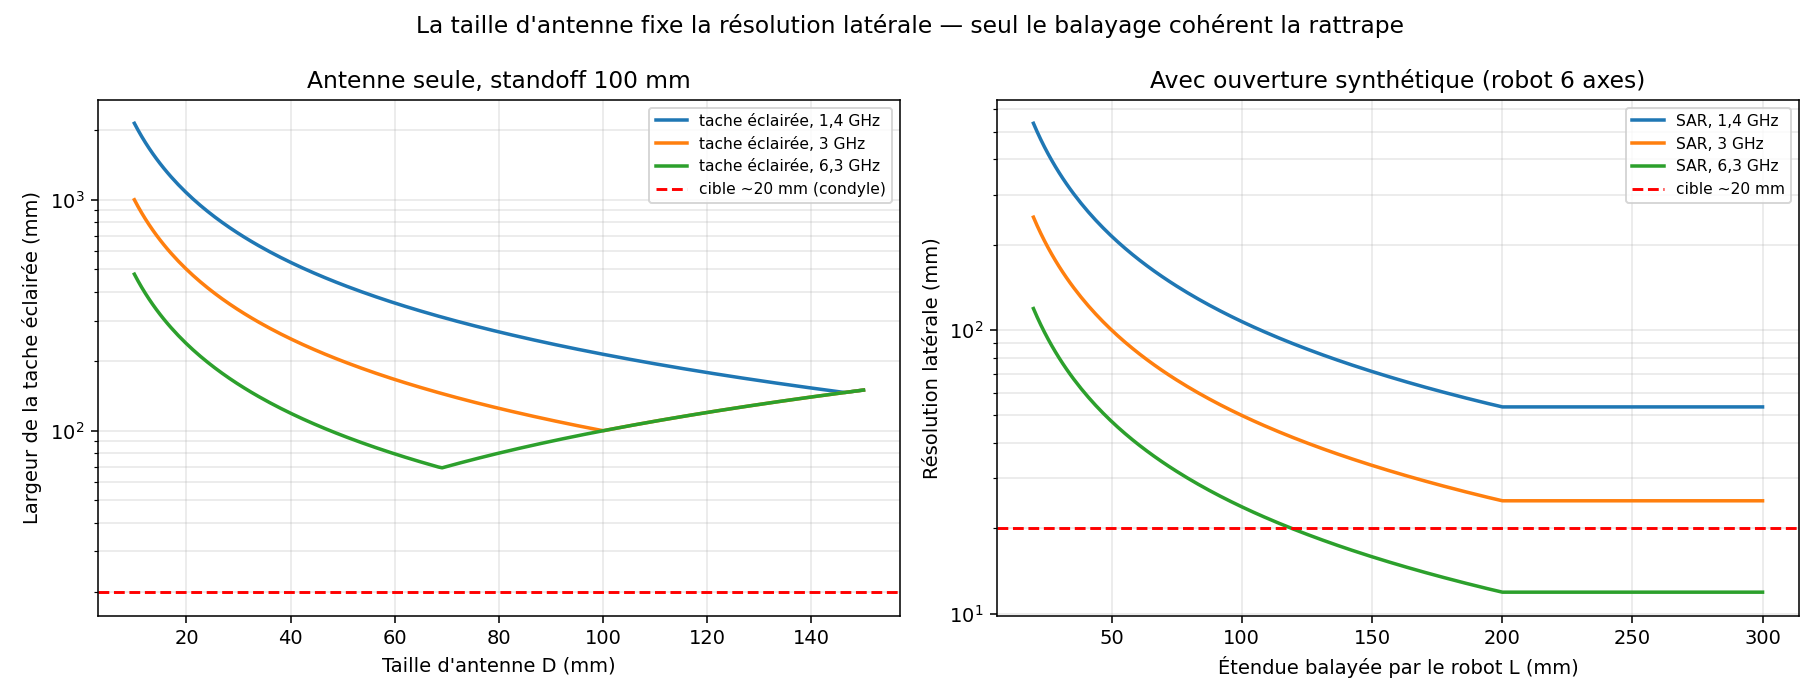
\includegraphics[width=0.96\textwidth]{fig_lateral.png}
\end{center}

\subsection{L'ouverture synthétique : la seule issue}

Le robot connaît sa pose exactement. On peut donc \emph{combiner de façon
cohérente} les mesures acquises en $M$ positions, exactement comme un radar à
ouverture synthétique.

L'expression que l'on rencontre le plus souvent, $\delta x \simeq \lambda R/2L$,
est la limite \emph{petits angles}. Elle cesse d'être valable dès que
l'ouverture $L$ devient comparable à la distance $R$ --- ce qui est précisément
notre cas si l'on travaille à $20$~mm de la surface. L'expression exacte fait
intervenir l'angle d'intégration $\theta$ sous lequel l'ouverture est vue depuis
la cible :

\begin{equation}
\boxed{\;\delta x \;=\; \frac{\lambda}{4\sin(\theta/2)}\;,
\qquad \theta \;=\; 2\arctan\!\frac{L}{2R}\;}
\label{eq:dx_exact}
\end{equation}

Elle \textbf{sature à $\lambda/4$} lorsque l'ouverture enveloppe complètement
l'objet ($\theta \to 180^\circ$). Cette borne est celle de la diffraction :
aucune ouverture, aucun traitement, aucun rapport signal à bruit ne la franchit.
À $6{,}3$~GHz elle vaut $11{,}9$~mm.

\begin{center}
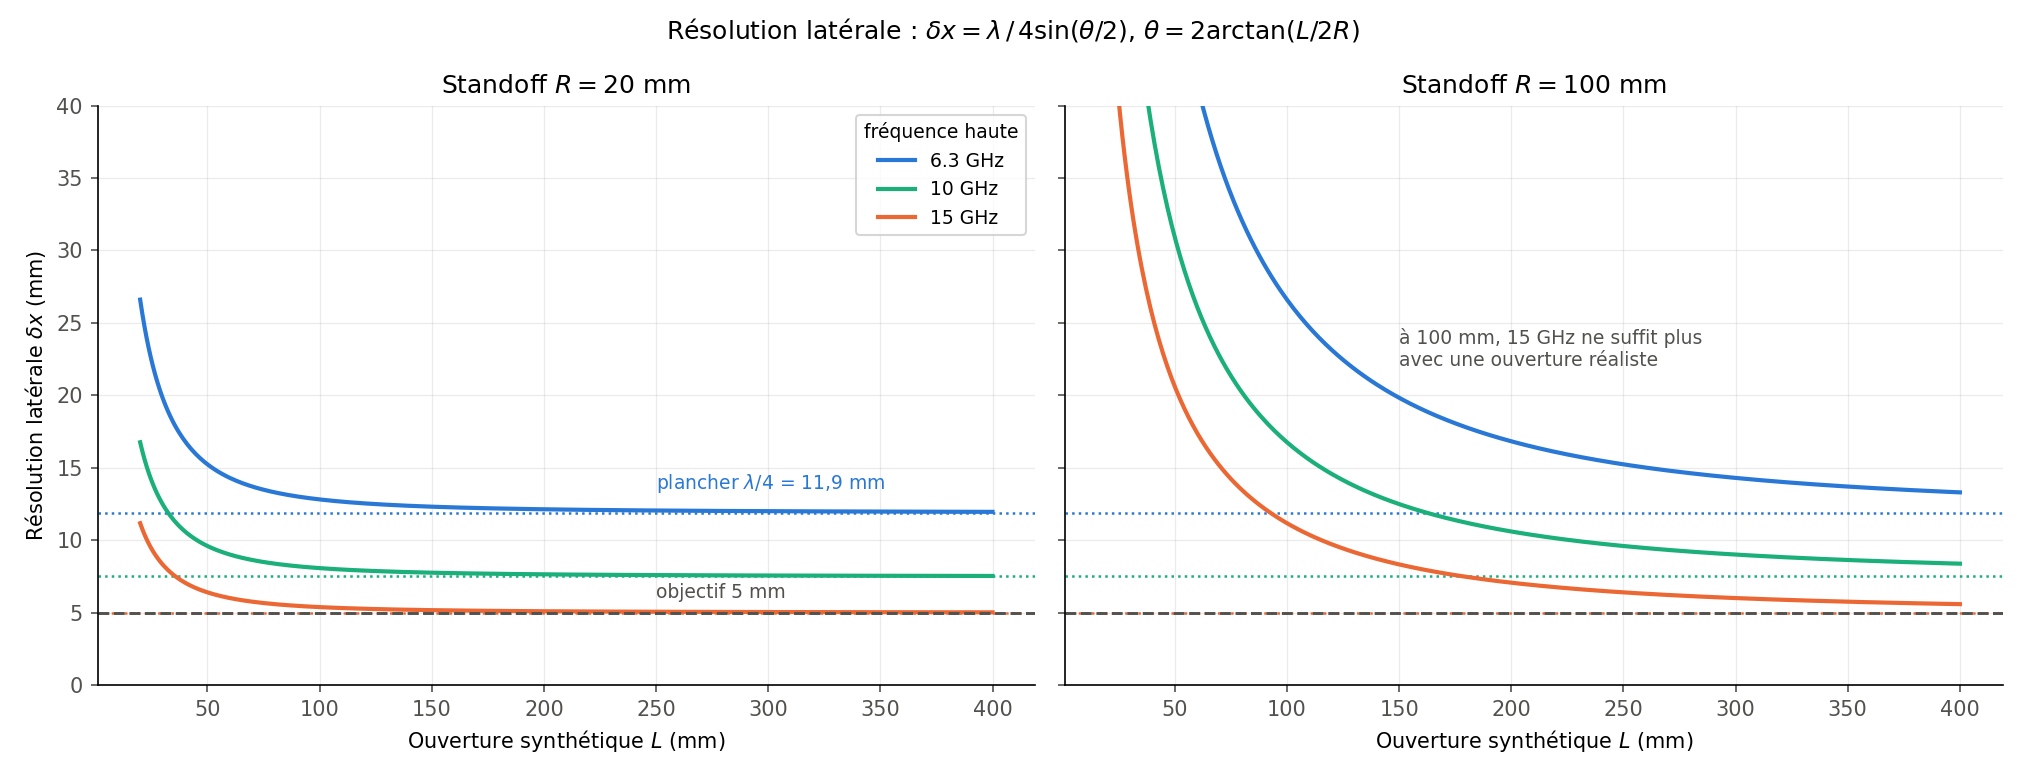
\includegraphics[width=\textwidth]{fig_laterale_exacte.png}
\end{center}

\begin{table}[h]
\centering
\caption{Résolution latérale (mm) donnée par~\eqref{eq:dx_exact} à
$6{,}3$~GHz.}
\begin{tabular}{lccc}
\toprule
Ouverture $L$ & $R = 20$~mm & $R = 30$~mm & $R = 50$~mm \\
\midrule
$60$~mm  & $14{,}3$ & $16{,}8$ & $23{,}1$ \\
$100$~mm & $12{,}8$ & $13{,}9$ & $16{,}8$ \\
$200$~mm & $12{,}1$ & $12{,}4$ & $13{,}3$ \\
$600$~mm & $11{,}9$ & $12{,}0$ & $12{,}1$ \\
\bottomrule
\end{tabular}
\end{table}

La saturation est brutale : au-delà d'une centaine de millimètres d'ouverture,
allonger le balayage ne rapporte plus rien. Le chiffre de travail est
$12$--$13$~mm.

\subsection{Pourquoi la forte permittivité ne rattrape pas}

L'objection naturelle est que la longueur d'onde dans le cartilage ne vaut que
$\lambda/\sqrt{\eps} = 7{,}3$~mm, ce qui donnerait $\lambda_2/4 = 1{,}8$~mm. Elle
ne tient pas, et la raison est instructive : \textbf{la composante transverse du
vecteur d'onde se conserve à la traversée de l'interface}. Une onde rasante dans
l'air ($90^\circ$) se réfracte à seulement

\begin{equation}
\theta_2 = \arcsin\frac{1}{\sqrt{\eps}} = \arcsin\frac{1}{6{,}52}
         = 8{,}8^\circ
\end{equation}

L'éventail angulaire disponible \emph{à l'intérieur} du milieu est donc
minuscule, et la réfraction annule exactement le gain de longueur d'onde :

\begin{equation}
\frac{\lambda_2}{4\sin\theta_2} = \frac{7{,}3}{4 \times 0{,}153}
= 11{,}9~\text{mm}
\end{equation}

identique au chiffre côté air. La permittivité élevée améliore la résolution
\emph{en profondeur}, jamais la résolution latérale.

\begin{implication}
La mesure est fortement \emph{anisotrope} : quelques centièmes de millimètre en
profondeur, mais $12$ à $13$~mm latéralement. Il faut distinguer résolution et
échantillonnage : on peut mesurer tous les $2$~mm, ce que la résolution limite
est le contenu en fréquences spatiales de la carte d'épaisseur, pas la densité
de points. L'épaisseur cartilagineuse varie à l'échelle du condyle ($50$ à
$70$~mm) : cette composante est intégralement restituée. Ce qui est perdu, ce
sont les lésions focales de moins d'un centimètre, vues comme un amincissement
étalé et atténué. Atteindre $5$~mm exigerait $\lambda \le 20$~mm, donc un
instrument allant à $15$~GHz (\S\ref{sec:bande}).
\end{implication}

\subsection{L'effet de volume partiel}

Si l'épaisseur varie de $\Delta d$ sous l'empreinte de l'antenne, les
contributions élémentaires se somment avec des phases différentes et la
signature se brouille. La perte de contraste suit

\begin{equation}
C(\Delta d) \;\simeq\;
   \left|\operatorname{sinc}\!\left(\beta_2 \Delta d/\pi\right)\right|,
\qquad \beta_2 = \frac{2\pi f\sqrt{\eps}}{c}
\end{equation}

\begin{center}
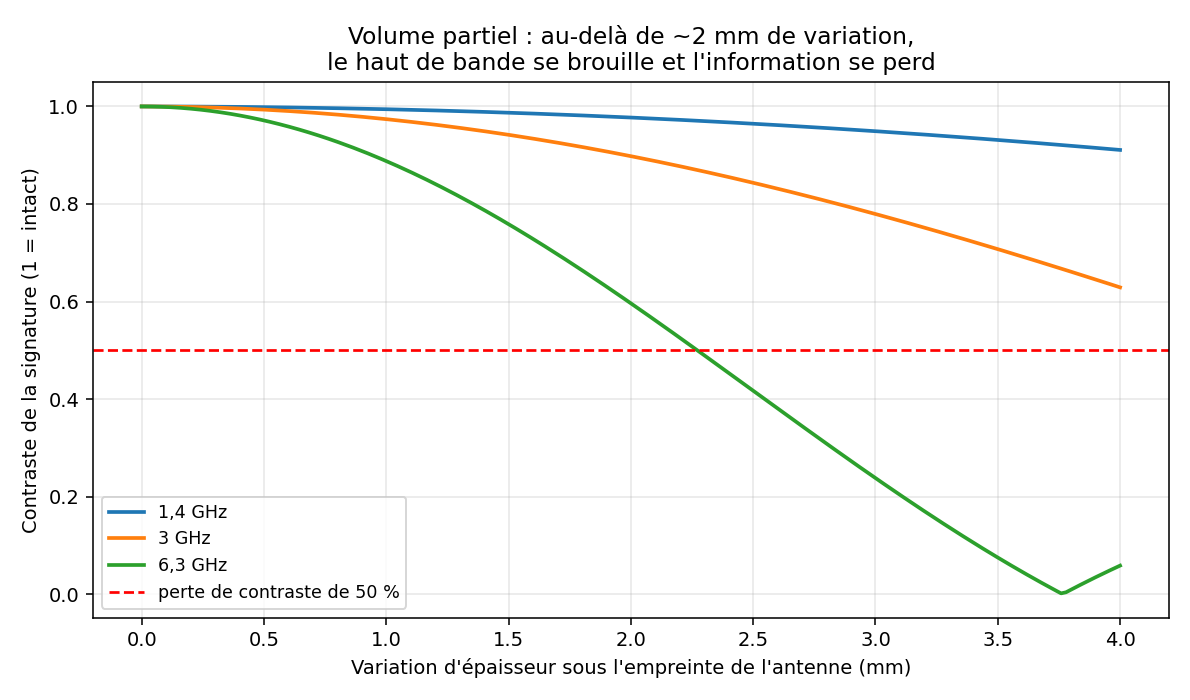
\includegraphics[width=0.72\textwidth]{fig_volume_partiel.png}
\end{center}

\begin{table}[h]
\centering
\begin{tabular}{lc}
\toprule
Fréquence & Variation d'épaisseur qui annule le contraste \\
\midrule
$1{,}4$~GHz & $16{,}9$~mm \\
$3$~GHz     & $7{,}9$~mm \\
$6{,}3$~GHz & $3{,}8$~mm \\
\bottomrule
\end{tabular}
\end{table}

\begin{implication}
L'empreinte de l'antenne doit être assez petite pour que l'épaisseur ne varie
pas de plus de $2$ à $3$~mm en son sein, faute de quoi le haut de bande --- qui
porte l'essentiel de l'information, cf.~\S\ref{sec:hautbande} --- se brouille.
Sur un condyle, cela impose une empreinte effective de l'ordre de $15$ à
$20$~mm, donc impérativement un traitement à ouverture synthétique. C'est la
justification quantitative du balayage robotisé.
\end{implication}

%=======================================================================
\section{Bande passante et résolution axiale}
%=======================================================================

\subsection{La dualité temps--fréquence}

Le VNA mesure $S_{11}(f)$ en $N$ points ; le profil en distance s'obtient par
transformée de Fourier inverse. Une fenêtre spectrale de largeur $B$ ne peut
produire une impulsion plus courte que $\tau \simeq 1/B$. En distance, avec le
facteur~2 de l'aller-retour :

\begin{equation}
\boxed{\;\delta r = \frac{c\tau}{2} = \frac{c}{2B}
  = \frac{3\times10^{8}}{2\times4{,}9\times10^{9}} = 30{,}6~\text{mm}\;}
\label{eq:rayleigh}
\end{equation}

$\delta r$ est la \emph{longueur de l'impulsion radar dans l'espace}. Dans un
milieu de permittivité $\eps$, elle devient $c/(2B\sqrt{\eps})$, soit
$4{,}8$~mm dans le cartilage --- $8{,}4$~mm en tenant compte de
l'élargissement dû à la fenêtre de Hann.

\begin{center}
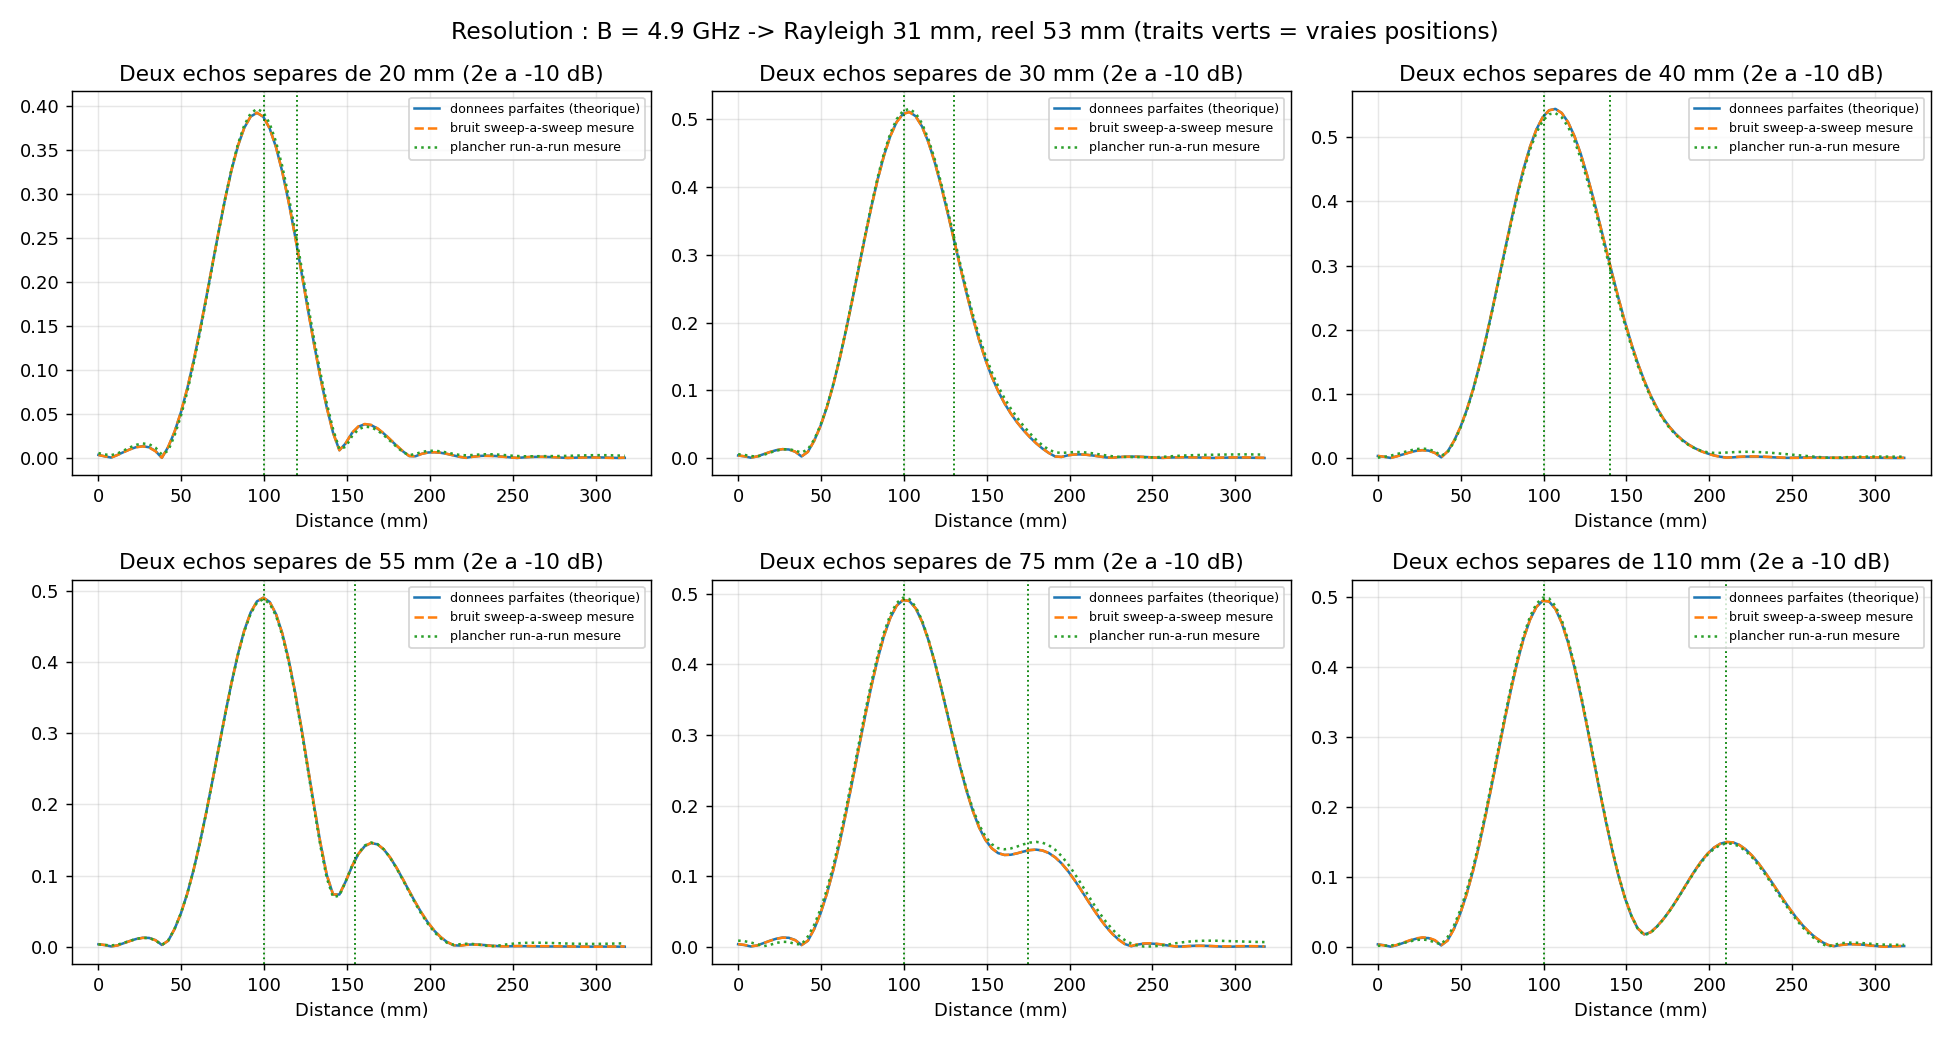
\includegraphics[width=\textwidth]{demo_resolution.png}
\end{center}

\subsection{Deux illusions}

\paragraph{Le remplissage par des zéros.} Notre facteur d'interpolation $Z=8$
donne un pas d'affichage de $3{,}83$~mm. Ce n'est pas la résolution : aucune
information n'est ajoutée. C'est le piège des fiches techniques annonçant
« résolution 6~mm » là où le chiffre désigne un pas d'échantillonnage.

\paragraph{Le nombre de points.} Augmenter $N$ à $B$ constant n'améliore que la
portée non ambiguë.

\begin{implication}
Par séparation de deux pics, la mesure d'un cartilage de $0$ à $5$~mm est
\emph{impossible} : il faudrait $7{,}9$~GHz de bande pour $3$~mm et $23{,}7$~GHz
pour $1$~mm. Le LiteVNA plafonne à $6{,}3$~GHz. Toute la suite consiste à ne
plus poser la question sous cette forme.
\end{implication}

%=======================================================================
\section{Trois grandeurs qu'il ne faut pas confondre}
%=======================================================================

\begin{table}[h]
\centering
\renewcommand{\arraystretch}{1.35}
\begin{tabular}{p{2.3cm}p{3.8cm}p{2.2cm}p{2.3cm}p{2.4cm}}
\toprule
Grandeur & Question posée & Fixée par & Formule & Notre valeur \\
\midrule
\textbf{Résolution} & « un ou deux échos ? » &
  bande $B$ & $c/2B$ & $30{,}6$ (53)~mm \\
\textbf{Portée} & « jusqu'où ? » &
  pas $\Delta f$ & $c/2\Delta f$ & $3060$~mm \\
\textbf{Précision} & « où est le centre ? » &
  $\mathrm{SNR}$ & $\propto \delta r/\sqrt{\mathrm{SNR}}$ & $0{,}008$~mm \\
\bottomrule
\end{tabular}
\end{table}

La limite de $30$~mm est un \emph{plancher} sur l'épaisseur séparable, non un
plafond : le plafond vaut $3$~m dans l'air. Une couche épaisse est facile ;
c'est la couche mince qui est difficile.

%=======================================================================
\section{Pourquoi précision et résolution divergent}
%=======================================================================

Localiser un écho de forme \emph{connue} est un problème d'estimation. La borne
de Cramér--Rao sur un retard $\tau$ s'écrit

\begin{equation}
\operatorname{var}(\hat\tau) \;\geq\;
   \frac{1}{2\,\mathrm{SNR}\,\beta_{\text{rms}}^{2}},
\qquad
\beta_{\text{rms}}^{2} =
   \frac{\int \omega^{2}|S(\omega)|^{2}\,\mathrm{d}\omega}
        {\int |S(\omega)|^{2}\,\mathrm{d}\omega}
\end{equation}

soit, à un facteur d'ordre unité près,

\begin{equation}
\boxed{\;\sigma_r \;\sim\; \frac{\delta r}{\sqrt{\mathrm{SNR}}}\;}
\label{eq:crb}
\end{equation}

Les deux grandeurs \emph{sont} liées --- mais la précision vaut la résolution
divisée par la racine du rapport signal/bruit. À $50$~dB, ce diviseur dépasse
$300$.

Séparer deux échos est en revanche un problème de \emph{sélection de modèle} :
quand l'écart tend vers zéro, le modèle à deux échos devient indiscernable du
modèle à un écho, l'information de Fisher associée s'annule et la variance
diverge. La limite de résolution s'améliore avec le SNR, mais beaucoup plus
lentement que~\eqref{eq:crb}.

\begin{implication}
Sur notre banc, l'écho d'antenne est une bosse large de $53$~mm dont nous
localisons le centre à $0{,}008$~mm près : un rapport de $6\,600$. Le critère de
Rayleigh~\eqref{eq:rayleigh} n'est pas une loi physique mais une convention.
Toute la stratégie du projet consiste à poser des questions d'estimation, où
nous sommes excellents, plutôt que des questions de résolution, où nous sommes
bloqués.
\end{implication}

%=======================================================================
\section{Méthodes paramétriques}
\label{sec:esprit}
%=======================================================================

Une somme de $K$ échos ponctuels s'écrit exactement comme une somme
d'exponentielles complexes,

\begin{equation}
s[n] = \sum_{k=1}^{K} a_k z_k^{\,n},
\qquad
z_k = \exp\!\left(-\jj\,\frac{4\pi \Delta f\, d_k}{c}\right)
\end{equation}

modèle canonique de MUSIC, ESPRIT et de la méthode matrice--faisceau. Leur
pouvoir séparateur dépend du rapport signal/bruit et de la connaissance de
l'ordre $K$ --- ici égal à $2$, et \emph{connu} grâce au relevé optique.

\begin{center}
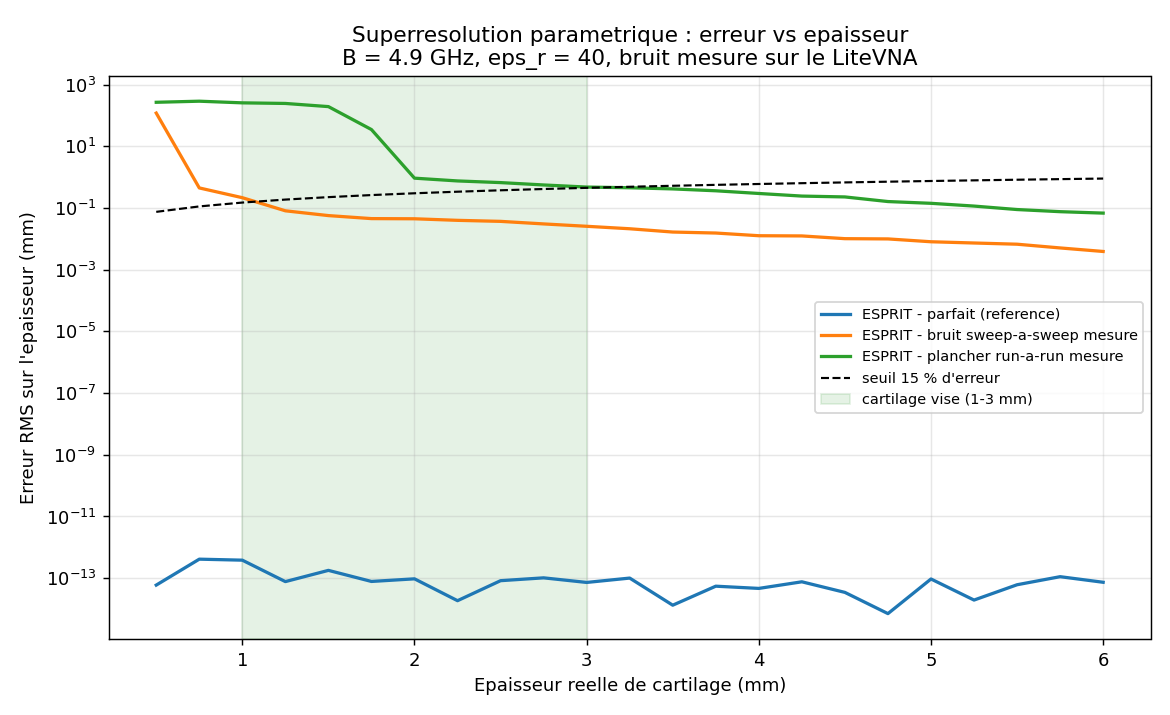
\includegraphics[width=0.78\textwidth]{superresolution.png}
\end{center}

%=======================================================================
\section{L'inversion sur modèle stratifié}
\label{sec:inversion}
%=======================================================================

\subsection{Le modèle}

\begin{center}
\begin{tikzpicture}[scale=1.05]
  \fill[blue!8] (0,1.5) rectangle (8,2.6);
  \fill[orange!18] (0,0) rectangle (8,1.5);
  \fill[gray!30] (0,-1.1) rectangle (8,0);
  \draw[very thick] (0,1.5) -- (8,1.5);
  \draw[very thick] (0,0) -- (8,0);
  \node[right] at (8.1,2.05) {air \; $n_1 = 1$};
  \node[right] at (8.1,0.75) {cartilage \; $n_2$, épaisseur $d$};
  \node[right] at (8.1,-0.55) {os \; $n_3$};
  \draw[<->, thick] (0.45,0) -- (0.45,1.5);
  \node[left] at (0.42,0.75) {$d$};
  % onde incidente et reflexions
  \draw[-{Latex[length=2mm]}, very thick, blue] (2.0,2.55) -- (2.5,1.55);
  \node[blue, above left] at (2.05,2.5) {\small incidente};
  \draw[-{Latex[length=2mm]}, very thick, red] (2.55,1.55) -- (3.05,2.55);
  \node[red, above right] at (3.0,2.5) {\small $r_{12}$};
  \draw[thick, dashed, orange!70!black] (2.5,1.5) -- (3.25,0);
  \draw[thick, dashed, orange!70!black] (3.25,0) -- (4.0,1.5);
  \draw[-{Latex[length=2mm]}, very thick, red!70] (4.0,1.5) -- (4.5,2.55);
  \node[red!70, above right] at (4.45,2.5) {\small $r_{23}\,\ee^{-2\jj\beta_2 d}$};
  \draw[thick, dotted, orange!70!black] (4.0,1.5) -- (4.75,0);
  \draw[thick, dotted, orange!70!black] (4.75,0) -- (5.5,1.5);
  \draw[-{Latex[length=2mm]}, thick, red!40] (5.5,1.5) -- (6.0,2.55);
  \node[red!40, above right] at (5.9,2.5) {\small réflexions multiples};
\end{tikzpicture}
\end{center}

La sommation de toutes les réflexions internes donne la forme close

\begin{equation}
\boxed{\;
\Gamma(f) = \frac{r_{12} + r_{23}\,\ee^{-2\jj\beta_2 d}}
                 {1 + r_{12} r_{23}\,\ee^{-2\jj\beta_2 d}}
\;}
\label{eq:gamma}
\end{equation}

\begin{equation}
r_{ij} = \frac{n_i - n_j}{n_i + n_j},
\qquad
\beta_2 = \frac{2\pi f}{c}\,n_2,
\qquad
n = \sqrt{\eps - \jj\,\frac{\sigma}{\omega \epsilon_0}}
\end{equation}

L'indice $n$ est \emph{complexe} : il encode le ralentissement de l'onde et son
absorption. Le modèle traite donc nativement la dispersion et les pertes.

\subsection{Ce que voit la mesure}

\begin{center}
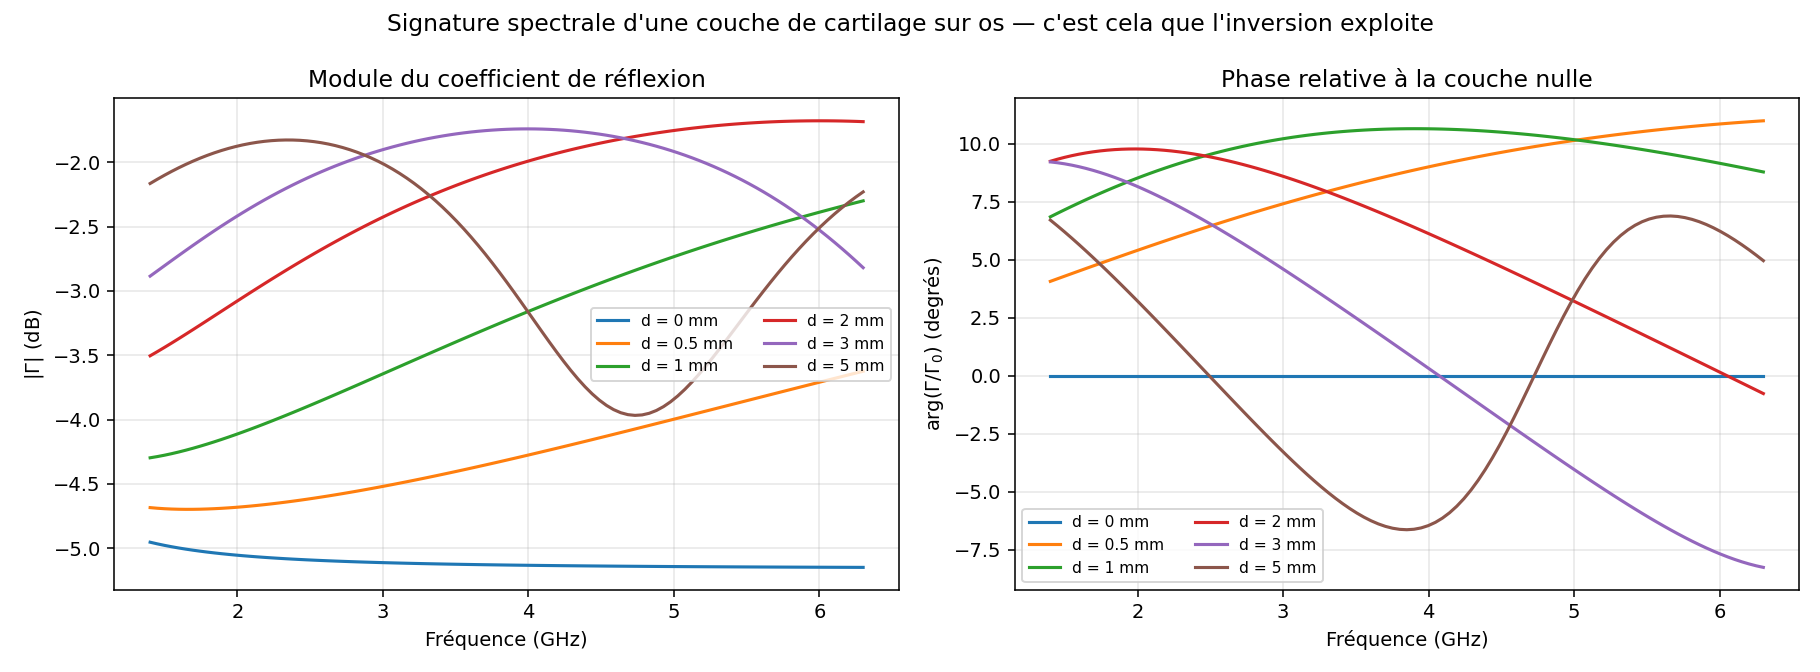
\includegraphics[width=\textwidth]{fig_signature.png}
\end{center}

Pour $d = 5$~mm à $6{,}3$~GHz, $2\beta_2 d \simeq 8{,}3$~rad : on observe plus
d'une frange complète. Pour $d = 0{,}2$~mm, $2\beta_2 d \simeq 0{,}33$~rad : on
est dans le régime linéaire. La bande couvre donc les deux régimes.

\subsection{L'estimateur}

En laissant libre un facteur complexe $K$ (gain et phase résiduels), l'estimateur
du maximum de vraisemblance est un \emph{filtre adapté sur l'épaisseur} :

\begin{equation}
\hat d = \arg\max_{d}\;
   \frac{\left|\langle \Gamma_{\text{mod}}(d),\, \Gamma_{\text{mes}}\rangle\right|^{2}}
        {\|\Gamma_{\text{mod}}(d)\|^{2}}
\end{equation}

En pratique le retard de standoff $\tau_0$ est lui aussi inconnu
(\S\ref{sec:standoff}), et le critère se maximise sur le couple $(d, \tau_0)$.
Cette surface est \emph{fortement non convexe} : une descente locale se piège
systématiquement. L'implantation
(\texttt{radar.py}, \S\ref{sec:programme}) procède donc par grille
grossière en $(d, \tau_0)$, $K$ étant éliminé analytiquement par projection à
chaque n\oe ud, puis raffine par simplexe. Validée sur données synthétiques, elle
restitue l'épaisseur vraie à $0{,}000$~mm de $1$ à $80$~mm.

\subsection{Valeurs de notre scène}

\begin{table}[h]
\centering
\begin{tabular}{lc}
\toprule
Réflexion air/cartilage $|r_{12}|$ & $0{,}732$ (54\,\% de la puissance) \\
Réflexion cartilage/os $|r_{23}|$  & $0{,}298$ \\
Écho de fond / écho de surface     & $-14{,}5$~dB \\
Atténuation aller-retour dans $3$~mm & $-2{,}6$~dB \\
\bottomrule
\end{tabular}
\end{table}

%=======================================================================
\section{La couche mince : pourquoi l'erreur n'explose pas}
\label{sec:couchemince}
%=======================================================================

C'est le résultat central. Pour $|2\beta_2 d| \ll 1$, en posant
$u = \ee^{-2\jj\beta_2 d}$ et en dérivant \eqref{eq:gamma} :

\begin{equation}
\boxed{\;
\Gamma(f) \;\simeq\; \Gamma_0
  \;-\; 2\jj\beta_2 d\;
  \frac{r_{23}\left(1 - r_{12}^{2}\right)}{\left(1 + r_{12}r_{23}\right)^{2}}
  \;+\; \mathcal{O}(d^{2})
\;}
\label{eq:mince}
\end{equation}

Trois conséquences :

\begin{enumerate}
\item $\Gamma$ dépend \emph{linéairement} de $d$, et la sensibilité
      $\partial\Gamma/\partial d$ \textbf{ne s'annule pas} quand $d\to0$.
      L'information n'est pas dans une séparation temporelle qui disparaît, mais
      dans l'amplitude d'une perturbation proportionnelle à $d$.
\item L'erreur \emph{absolue} est donc à peu près constante en fonction de
      l'épaisseur : la limite de Rayleigh ne s'applique pas à cette question.
\item $\beta_2 \propto f$ : la perturbation croît avec la fréquence.
\end{enumerate}

%=======================================================================
\section{Où est l'information : le haut de bande}
\label{sec:hautbande}
%=======================================================================

L'information de Fisher sur $d$ a pour densité spectrale
$|\partial\Gamma/\partial d|^{2}$.

\begin{center}
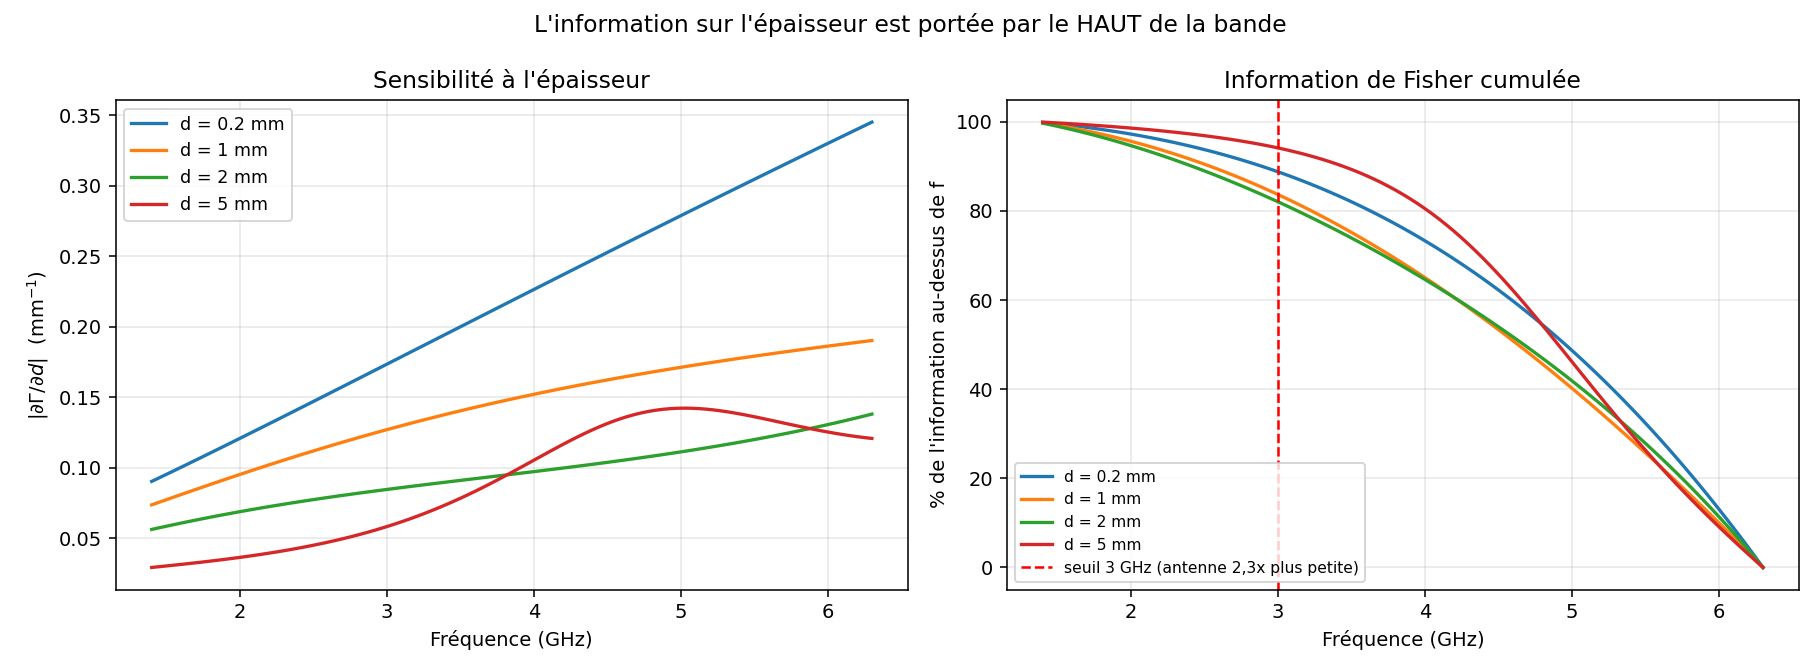
\includegraphics[width=\textwidth]{fig_sensibilite.png}
\end{center}

\begin{table}[h]
\centering
\begin{tabular}{lcccc}
\toprule
Épaisseur & $0{,}2$~mm & $1$~mm & $2$~mm & $5$~mm \\
\midrule
Part de l'information au-dessus de $3$~GHz
 & $89{,}1\,\%$ & $84{,}2\,\%$ & $82{,}5\,\%$ & $94{,}3\,\%$ \\
\bottomrule
\end{tabular}
\end{table}

\begin{implication}
Ce résultat résout la contrainte d'encombrement. Renoncer à la bande
$1{,}4$--$3$~GHz ne coûte que $6$ à $18\,\%$ de l'information sur l'épaisseur,
mais permet une antenne \textbf{$2{,}3$ fois plus petite} ($\simeq 50$~mm au lieu
de $107$~mm) --- ce qui change tout pour un champ opératoire et améliore
simultanément la résolution latérale et le volume partiel. \emph{Réserve} : les
basses fréquences aident à séparer $d$ de $\eps$ par le jeu de la dispersion ;
ce point n'est pas quantifié ici et doit être vérifié avant de trancher.
\end{implication}

%=======================================================================
\section{La dégénérescence épaisseur--permittivité}
%=======================================================================

Le terme de phase de \eqref{eq:gamma} s'écrit
$2\beta_2 d = (4\pi f/c)\sqrt{\eps}\,d$ : l'épaisseur et la permittivité n'y
apparaissent que par le produit $d\sqrt{\eps}$, dit \emph{épaisseur électrique}.
Seuls les modules $r_{12}$ et $r_{23}$ brisent faiblement cette dégénérescence.
D'où

\begin{equation}
\boxed{\;\frac{\delta d}{d} \;\simeq\; -\frac{1}{2}\,\frac{\delta \eps}{\eps}\;}
\end{equation}

\begin{center}
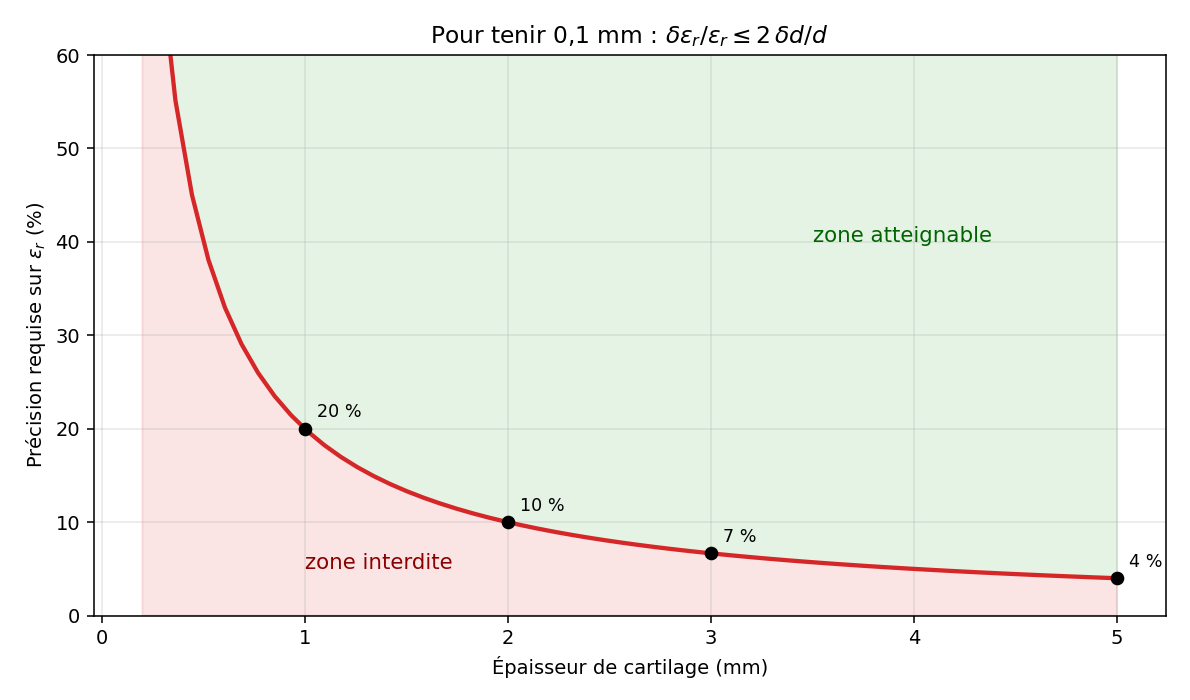
\includegraphics[width=0.72\textwidth]{fig_eps_requis.png}
\end{center}

\begin{implication}
Pour tenir $0{,}1$~mm à $d = 5$~mm, il faut connaître $\eps$ à $4\,\%$ ; à
$d = 1$~mm, $20\,\%$ suffisent. \textbf{C'est donc le cartilage épais qui est le
cas difficile}, à l'inverse de l'intuition. La permittivité du cartilage variant
avec l'hydratation, la température et l'état du tissu, une mesure indépendante
de $\eps$ sur le patient devient un préalable et non un raffinement.
\end{implication}

%=======================================================================
\section{Le balayage robotisé : moyennage et ouverture synthétique}
%=======================================================================

Le robot acquiert de nombreuses poses. Si l'échantillonnage spatial est plus
fin que la résolution latérale, le lissage local moyenne $M$ mesures
indépendantes et le bruit aléatoire décroît en $1/\sqrt{M}$.

\begin{center}
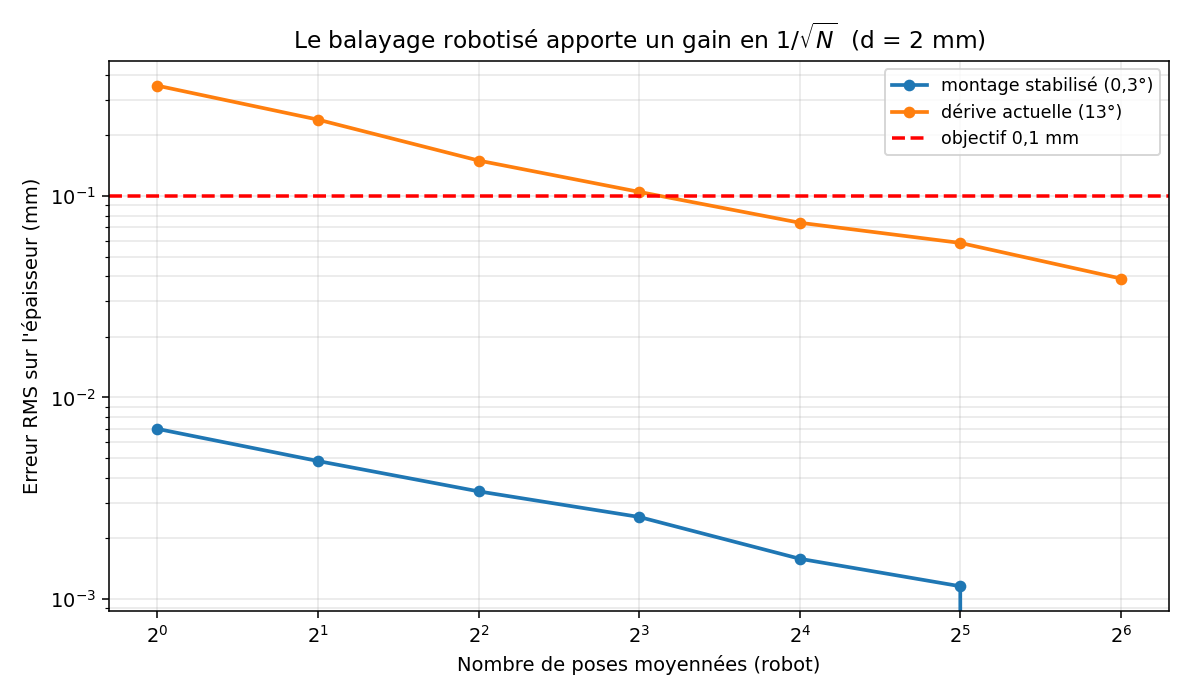
\includegraphics[width=0.72\textwidth]{fig_moyennage.png}
\end{center}

\begin{implication}
Le sur-échantillonnage spatial n'est pas seulement utile pour l'ouverture
synthétique : il achète directement de la précision en profondeur. Nous avons
par ailleurs vérifié expérimentalement que la dérive de notre montage est
décorrélée en fréquence ($0{,}1$ à $5{,}5\,\%$ seulement de sa variance
s'explique par une rampe de phase), donc qu'elle se moyenne. Si elle avait été
un retard pur, elle aurait imité une variation d'épaisseur et rien n'aurait pu
l'en distinguer.
\end{implication}

%=======================================================================
\section{Le traitement à ouverture synthétique}
\label{sec:sar}
%=======================================================================

\subsection{Le renversement de perspective}

Le \S\ref{sec:lateral} présentait la largeur d'empreinte comme un défaut. En
traitement cohérent, c'est l'inverse : \textbf{un faisceau large est un
avantage}. Un point $\mathbf{P}$ de la surface éclairé par une antenne large est
vu depuis \emph{de nombreuses positions successives} au fil de la translation,
donc sous de nombreux angles. Cette diversité angulaire est exactement ce qui
construit l'ouverture synthétique.

\begin{center}
\begin{tikzpicture}[scale=1.0]
  \draw[very thick, blue!70!black] (0,0) .. controls (2.5,0.55) and (5.5,0.55) .. (8,0);
  \node[blue!70!black, right] at (8.1,0) {\small surface connue};
  \foreach \x in {1.0,2.2,3.4,4.6,5.8,7.0} {
    \draw[fill=gray!25, thick] (\x-0.28,2.35) rectangle (\x+0.28,2.62);
    \draw[dashed, gray] (\x,2.35) -- (4.0,0.42);
  }
  \fill[red] (4.0,0.42) circle (2.2pt);
  \node[red, below] at (4.0,0.33) {\small $\mathbf{P}$};
  \draw[-{Latex[length=2mm]}, thick] (0.6,2.85) -- (7.4,2.85);
  \node[above] at (4.0,2.88) {\small $M$ poses connues exactement --- étendue $L$};
  \draw[<->, thick] (8.4,0.42) -- (8.4,2.35);
  \node[right] at (8.45,1.4) {\small $R$};
\end{tikzpicture}
\end{center}

\subsection{Rétroprojection cohérente}

L'algorithme générique consiste à sommer, pour chaque point candidat
$\mathbf{x}$, les contributions de toutes les poses recalées de leur retard
propre :

\begin{equation}
I(\mathbf{x}) \;=\; \sum_{m=1}^{M}\sum_{k=1}^{N}
   w_{mk}\; S_{11}^{(m)}(f_k)\;
   \exp\!\left(+\jj\,2\pi f_k\,\tau_m(\mathbf{x})\right),
\qquad
\tau_m(\mathbf{x}) = \frac{2\,\|\mathbf{x}-\mathbf{r}_m\|}{c}
\label{eq:bp}
\end{equation}

où $\mathbf{r}_m$ est la position de l'antenne à la pose $m$ et $w_{mk}$ une
pondération (apodisation d'ouverture, compensation d'étalement).

\subsection{La variante adaptée à notre problème}

L'équation~\eqref{eq:bp} cherche dans tout un volume. Or \emph{nous savons déjà
où est la surface}. Il est donc inutile de reconstruire une image : il suffit de
\textbf{focaliser exactement sur la surface connue}, puis d'estimer l'unique
paramètre restant.

Pour chaque point $\mathbf{P}$ du maillage optique, on compense le trajet dans
l'air, parfaitement connu :

\begin{equation}
\widetilde{\Gamma}_m(\mathbf{P},f) \;=\;
   \frac{S_{11}^{(m)}(f)}{A_m(\mathbf{P})}\;
   \exp\!\left(+\jj\,2\pi f\,\tau_m^{\text{air}}(\mathbf{P})\right)
\end{equation}

$A_m$ regroupant l'étalement géométrique et le diagramme d'antenne. Puis on
applique le filtre adapté sur l'épaisseur, en sommant \emph{de façon cohérente}
sur les poses qui éclairent $\mathbf{P}$ :

\begin{equation}
\boxed{\;
\hat d(\mathbf{P}) \;=\; \arg\max_{d}\;
   \frac{\left|\sum_{m} \big\langle
      \Gamma_{\text{mod}}(d,\theta_m),\,
      \widetilde{\Gamma}_m(\mathbf{P},\cdot)\big\rangle\right|^{2}}
        {\sum_{m}\big\|\Gamma_{\text{mod}}(d,\theta_m)\big\|^{2}}
\;}
\label{eq:sar-inv}
\end{equation}

C'est la fusion des deux idées du document : \emph{rétroprojection cohérente sur
une surface connue}, suivie de \emph{l'inversion du modèle stratifié}. Le gain
en rapport signal/bruit croît comme $M$ en puissance, donc l'écart-type sur
$\hat d$ décroît en $1/\sqrt{M}$.

\subsection{Incidence oblique}

Une pose $m$ voyant $\mathbf{P}$ sous l'angle $\theta_m$, le modèle de
\S\ref{sec:inversion} doit être généralisé. La constante de propagation normale
à l'interface devient, par la loi de Snell--Descartes,

\begin{equation}
\beta_{2z} = \frac{2\pi f}{c}\sqrt{n_2^{2} - \sin^{2}\theta_1}
\end{equation}

et les coefficients de Fresnel se scindent selon la polarisation :

\begin{equation}
r_{12}^{\text{TE}} =
  \frac{n_1\cos\theta_1 - n_2\cos\theta_2}{n_1\cos\theta_1 + n_2\cos\theta_2},
\qquad
r_{12}^{\text{TM}} =
  \frac{n_2\cos\theta_1 - n_1\cos\theta_2}{n_2\cos\theta_1 + n_1\cos\theta_2}
\end{equation}

\begin{implication}
Les six degrés de liberté permettent de présenter l'antenne normalement à la
surface, ce qui maximise le signal et simplifie le modèle --- mais supprime la
diversité angulaire dont vit le SAR. Le bon compromis est de \emph{translater}
l'antenne en gardant une orientation modérément variable, et d'accepter des
angles obliques dans le modèle. Une implantation qui n'utiliserait que
l'incidence normale se priverait de la résolution latérale.
\end{implication}

\subsection{Budget de cohérence}

La sommation cohérente n'est valide que si l'erreur de trajet reste petite
devant la longueur d'onde. Pour une erreur de pose RMS $\Delta r$, la phase
aller-retour a pour écart-type $\sigma_\varphi = 4\pi\Delta r/\lambda$ et la
perte vaut $8{,}686\,\sigma_\varphi^{2}$ dB.

\begin{center}
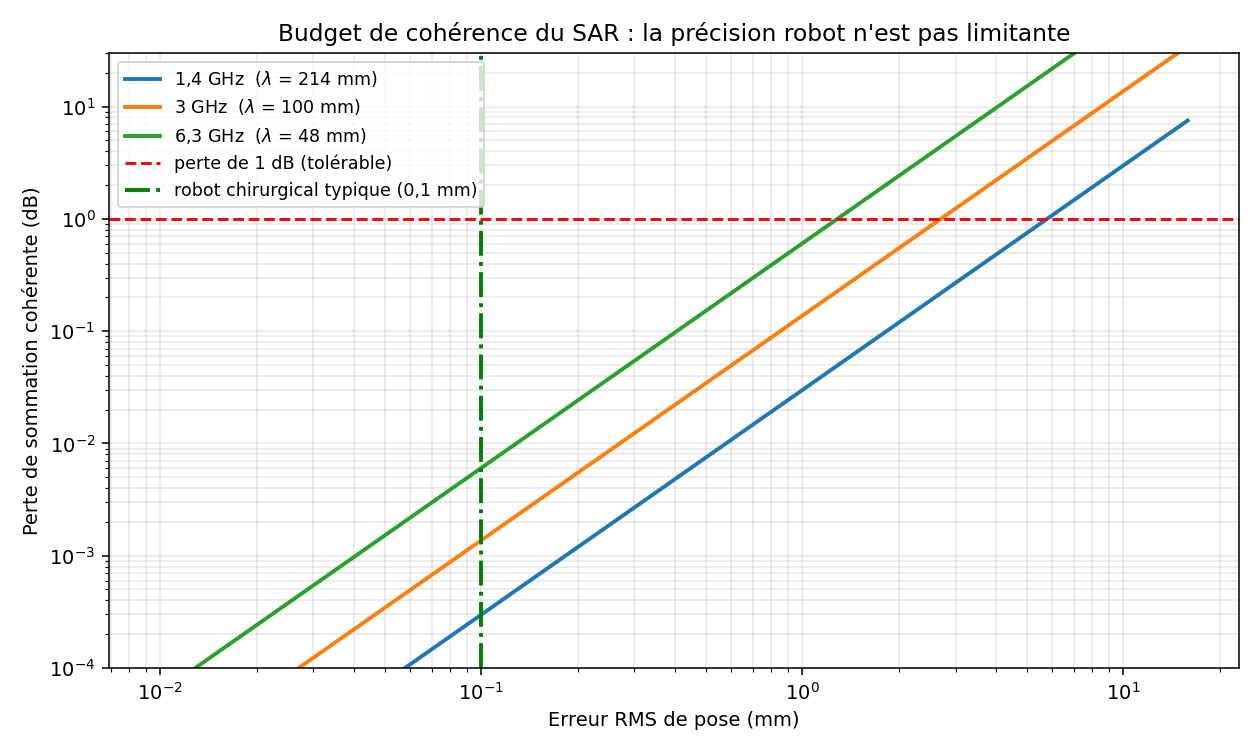
\includegraphics[width=0.78\textwidth]{fig_sar_coherence.png}
\end{center}

\begin{table}[h]
\centering
\begin{tabular}{lc}
\toprule
Fréquence & Erreur de pose donnant $1$~dB de perte \\
\midrule
$1{,}4$~GHz & $5{,}79$~mm \\
$3$~GHz     & $2{,}70$~mm \\
$6{,}3$~GHz & $1{,}29$~mm \\
\bottomrule
\end{tabular}
\end{table}

\begin{implication}
Un robot chirurgical à $0{,}1$~mm dispose d'un facteur $13$ de marge à
$6{,}3$~GHz. \textbf{La précision du robot n'est absolument pas limitante.} En
revanche la même tolérance s'applique aux \emph{mouvements du patient} : le
fémur doit être suivi par le système de navigation avec cette même exactitude,
faute de quoi la cohérence de l'ouverture est détruite. C'est la contrainte
opératoire réelle, et elle est satisfaite par les systèmes de navigation
existants.
\end{implication}

\subsection{Échantillonnage et durée du balayage}

Pour éviter les lobes de réseau, le pas d'échantillonnage de l'ouverture doit
respecter $\Delta x \leq \lambda_{\min}/4$.

\begin{center}
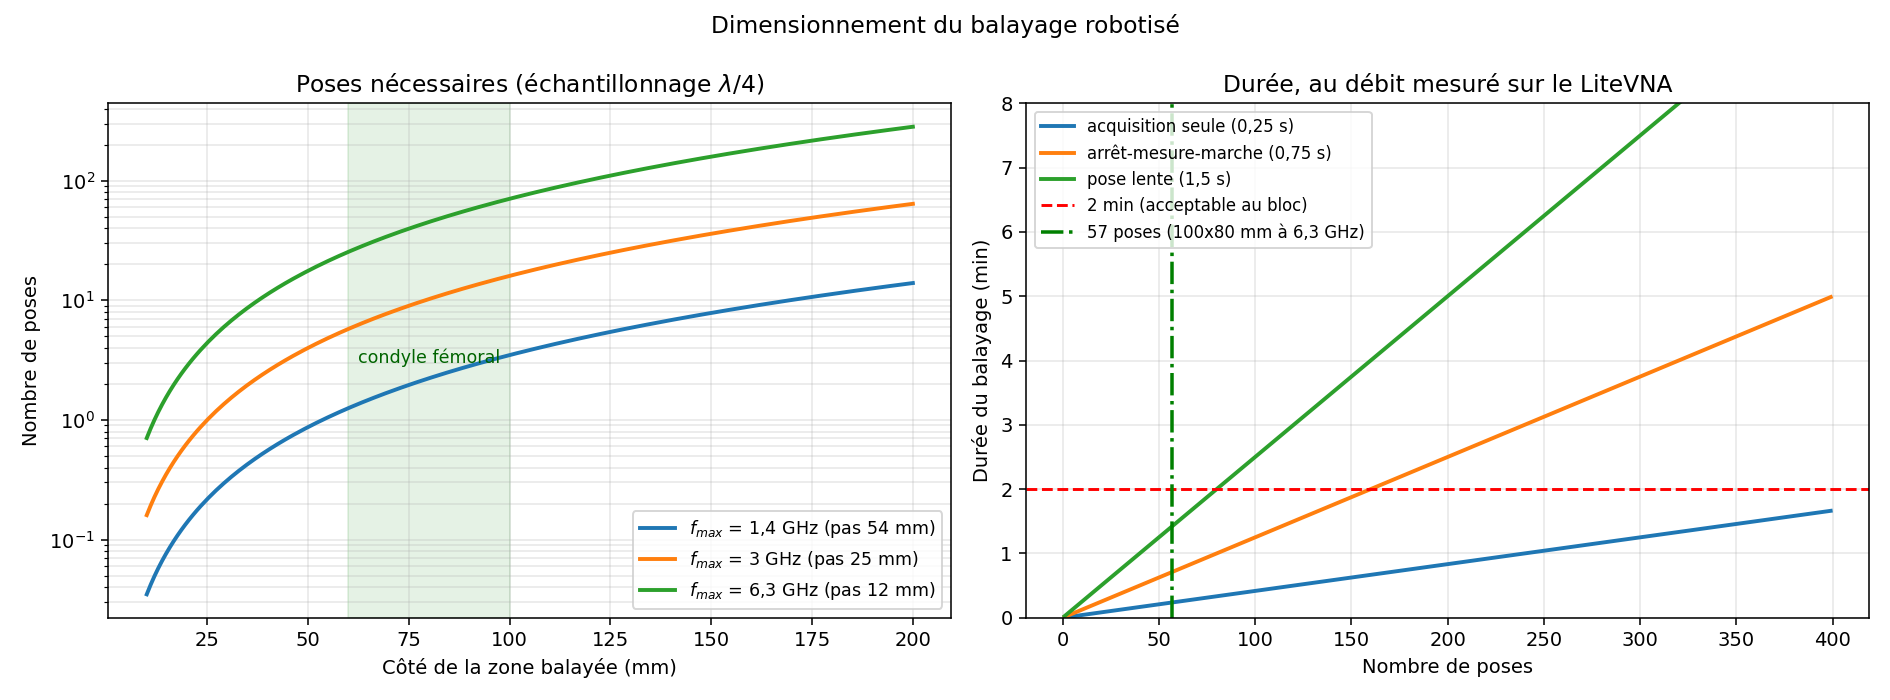
\includegraphics[width=\textwidth]{fig_sar_poses.png}
\end{center}

\begin{table}[h]
\centering
\begin{tabular}{lcc}
\toprule
$f_{\max}$ & Pas requis & Poses pour $100\times 80$~mm \\
\midrule
$1{,}4$~GHz & $53{,}6$~mm & $3$ \\
$3$~GHz     & $25{,}0$~mm & $13$ \\
$6{,}3$~GHz & $11{,}9$~mm & $56$ \\
\bottomrule
\end{tabular}
\end{table}

\begin{implication}
Couvrir un condyle demande environ \textbf{56 poses}. Au débit mesuré sur notre
LiteVNA ($0{,}25$~s par balayage) et avec une seconde de déplacement robot par
pose, le relevé complet tient en \textbf{moins d'une minute}. C'est compatible
avec une utilisation peropératoire --- et c'est le résultat le plus encourageant
de ces notes.
\end{implication}

%=======================================================================
\section{Budget d'erreur et faisabilité du dixième de millimètre}
%=======================================================================

\begin{center}
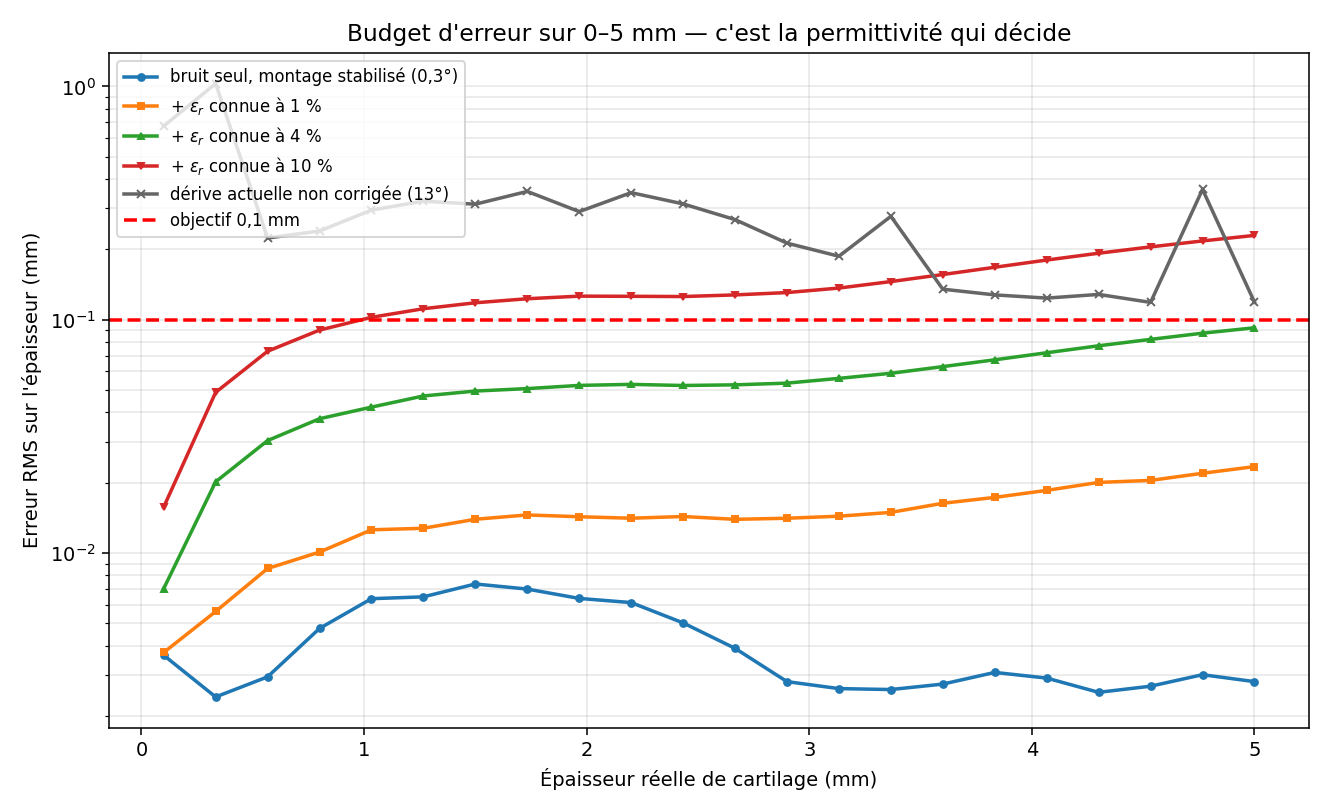
\includegraphics[width=\textwidth]{fig_budget.png}
\end{center}

\begin{table}[h]
\centering
\begin{tabular}{lcc}
\toprule
Configuration & Erreur sur $0$--$5$~mm & Objectif $0{,}1$~mm \\
\midrule
Dérive actuelle non corrigée ($13^\circ$) & $0{,}12$ à $0{,}40$~mm & échec \\
Stabilisé, $\eps$ à $10\,\%$              & $0{,}02$ à $0{,}25$~mm & échec au-delà de $1$~mm \\
Stabilisé, $\eps$ à $4\,\%$               & $0{,}007$ à $0{,}095$~mm & \textbf{atteint} \\
Stabilisé, $\eps$ à $1\,\%$               & $0{,}003$ à $0{,}024$~mm & large marge \\
Bruit seul (plancher théorique)           & $\simeq 0{,}005$~mm & --- \\
\bottomrule
\end{tabular}
\end{table}

\subsection{Conclusion de faisabilité}

\begin{center}
\fbox{\begin{minipage}{0.9\textwidth}
\centering
L'objectif de $0{,}1$~mm sur $0$--$5$~mm est \textbf{atteignable}, à deux
conditions strictes :\\[1mm]
(i) éliminer la dérive mécanique du montage ;\qquad
(ii) connaître $\eps$ à environ $4\,\%$.\\[1mm]
Le bruit de l'instrument n'est \emph{pas} le facteur limitant.
\end{minipage}}
\end{center}

\subsection{Risques non quantifiés}

\begin{enumerate}
\item \textbf{Film de liquide.} Une pellicule de sang ou de sérum
      physiologique ($\eps \simeq 78$) sur le cartilage constitue une couche
      supplémentaire et biaise l'inversion. C'est probablement le risque
      pratique le plus sérieux en conditions opératoires.
\item \textbf{Champ proche et courbure.} Le modèle d'onde plane en incidence
      normale est une approximation ; la courbure du condyle et la proximité de
      l'antenne introduisent des erreurs systématiques qu'un filtre adapté ne
      rejette pas.
\item \textbf{Ringing d'antenne.} Une antenne résonante allonge la réponse
      impulsionnelle et brouille l'ordre du modèle. Notre antenne actuelle
      présente $|S_{11}| = -6{,}6$~dB entre $4{,}2$ et $4{,}9$~GHz, soit
      $22\,\%$ de puissance réfléchie, précisément dans le haut de bande le plus
      informatif.
\item \textbf{Température.} $\eps$ du cartilage en dépend ; l'écart entre
      température ambiante et température corporelle doit être caractérisé.
\end{enumerate}

%=======================================================================
\section{Propriétés diélectriques : le modèle de Debye}
\label{sec:debye}
%=======================================================================

Tout ce qui précède suppose connue la permittivité complexe du milieu traversé.
Elle n'est pas un nombre mais une \emph{courbe}, et sa forme décide à elle seule
du choix de la bande (\S\ref{sec:bande}).

\subsection{L'idée physique}

Une molécule d'eau est un dipôle. Placée dans un champ électrique elle
s'oriente, mais elle possède de l'inertie et frotte contre ses voisines : elle
met un temps $\tau$ à le faire. Debye pose une hypothèse unique --- la
polarisation relaxe exponentiellement, avec une seule constante de temps :

\begin{equation}
\frac{\mathrm{d}P}{\mathrm{d}t} = -\frac{P - P_\infty}{\tau}
\end{equation}

Passée en fréquence, cette équation du premier ordre donne

\begin{equation}
\varepsilon(\omega) = \varepsilon_\infty
   + \frac{\varepsilon_s - \varepsilon_\infty}{1 + \jj\omega\tau}
\label{eq:debye}
\end{equation}

soit, en séparant partie réelle et partie imaginaire,

\begin{equation}
\varepsilon'(\omega) = \varepsilon_\infty
   + \frac{\Delta\varepsilon}{1+\omega^2\tau^2},
\qquad
\varepsilon''(\omega) = \frac{\Delta\varepsilon\,\omega\tau}{1+\omega^2\tau^2}
\end{equation}

Trois régimes se succèdent :

\begin{itemize}
\item $\omega \ll 1/\tau$ : les dipôles suivent sans effort,
      $\varepsilon' = \varepsilon_s$, pertes dipolaires nulles ;
\item $\omega \simeq 1/\tau$ : ils suivent \emph{en retard}. Le déphasage entre
      champ et polarisation dissipe de l'énergie et $\varepsilon''$ passe par un
      maximum valant $\Delta\varepsilon/2$ ;
\item $\omega \gg 1/\tau$ : ils n'ont plus le temps de bouger et décrochent,
      $\varepsilon' \to \varepsilon_\infty$.
\end{itemize}

Le pic de pertes se situe exactement à $\omega\tau = 1$, soit
$f = 1/2\pi\tau \simeq 19$~GHz pour l'eau tissulaire.

\subsection{Le second terme : la conduction ionique}

Il faut y ajouter un mécanisme \emph{différent} : les ions libres
($\mathrm{Na^+}$, $\mathrm{Cl^-}$) ne s'orientent pas, ils dérivent. Cela
constitue un vrai courant, donc une vraie dissipation, qui ne sature jamais et
diverge en $1/\omega$ vers les basses fréquences :

\begin{equation}
\varepsilon(\omega) = \varepsilon_\infty
   + \frac{\Delta\varepsilon}{1 + \jj\omega\tau}
   - \jj\,\frac{\sigma_i}{\omega\varepsilon_0}
\label{eq:debye_ion}
\end{equation}

Ce terme domine sous $1$~GHz et devient négligeable au-delà de $10$~GHz.

\subsection{L'ajustement retenu, et son statut}

Les quatre paramètres libres de~\eqref{eq:debye_ion} ont été choisis pour que la
formule passe par les valeurs publiées du cartilage :
$\varepsilon_s = 45$, $\varepsilon_\infty = 5$, $\tau = 8{,}5$~ps,
$\sigma_i = 0{,}9$~S/m.

\begin{table}[h]
\centering
\begin{tabular}{lll}
\toprule
& Modèle & Publié \\
\midrule
$2{,}45$~GHz & $\varepsilon' = 44{,}3$ ; $\sigma = 1{,}60$~S/m
             & $\simeq 42$ ; $1{,}6$ \\
$10$~GHz     & $\varepsilon' = 36{,}1$ ; $\sigma = 10{,}15$~S/m
             & $\simeq 32$ ; $9$ \\
\bottomrule
\end{tabular}
\end{table}

\begin{center}
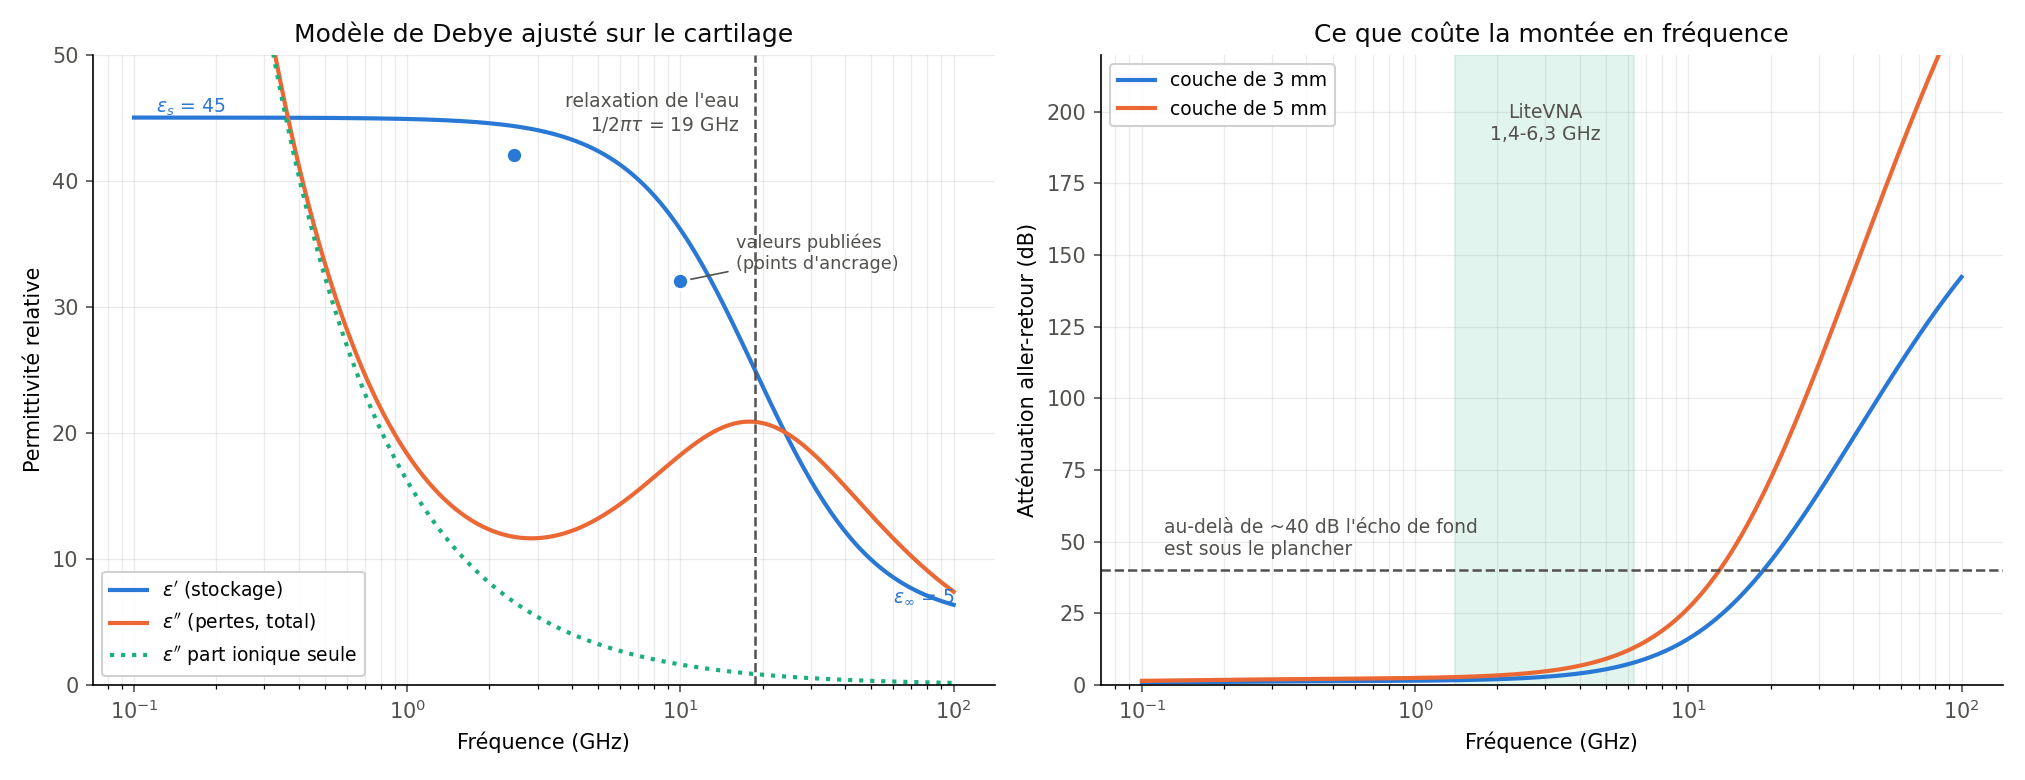
\includegraphics[width=\textwidth]{fig_debye.png}
\end{center}

Il s'agit donc d'une \textbf{interpolation contrainte par la physique}, non
d'une mesure : deux points d'ancrage pour quatre paramètres. Ce qui la rend
néanmoins fiable là où elle sert, c'est que la position du pic de pertes n'est
pas un paramètre libre --- elle est fixée par $\tau$, c'est-à-dire par l'eau,
connue à quelques pour cent. Le cartilage étant à $75\,\%$ d'eau, son absorption
\emph{doit} croître brutalement vers $20$~GHz. Les décibels calculés portent
sans doute $\pm 30\,\%$ ; la \emph{forme} de la courbe, elle, est certaine.

\subsection{Ses limites}

Un tissu réel ne possède pas une constante de temps mais une
\emph{distribution} : eau libre, eau liée au collagène et chaînes latérales des
protéines relaxent chacune différemment. On généralise par la forme de
Cole--Cole,

\begin{equation}
\varepsilon(\omega) = \varepsilon_\infty
   + \frac{\Delta\varepsilon}{1 + (\jj\omega\tau)^{1-\alpha}}
\end{equation}

où $\alpha$ élargit le pic ; le modèle de référence (Gabriel) empile quatre
termes de ce type plus la conduction pour couvrir $10$~Hz à $100$~GHz.

\begin{implication}
Un Debye unique suffit à une étude de faisabilité sur $1$--$70$~GHz. Il ne
suffira \emph{pas} à l'inversion finale, parce que $\eps$ intervient deux fois
dans l'épaisseur --- par la longueur d'onde dans la couche ($\sqrt{\eps}$) et
par les coefficients de Fresnel --- et parce que c'est une courbe et non un
nombre. Lorsque l'on écrit « $\eps$ connu à $4\,\%$ », c'est de la courbe
entière qu'il s'agit.
\end{implication}

%=======================================================================
\section{La gamme des milieux et la carte de faisabilité}
\label{sec:milieux}
%=======================================================================

\subsection{Les milieux visés}

\begin{table}[h]
\centering
\begin{tabular}{lll}
\toprule
Milieu & $\eps$ (2--5~GHz) & Teneur en eau \\
\midrule
Air              & $1{,}0$      & $0\,\%$ \\
Os cortical      & $10$ à $12$  & très faible \\
Os spongieux     & $18$ à $22$  & faible \\
Peau (sèche)     & $38$ à $40$  & moyenne \\
Cartilage        & $40$ à $45$  & élevée \\
Foie             & $43$ à $46$  & élevée \\
Sang             & $55$ à $60$  & très élevée \\
Eau pure         & $\simeq 78$ à $80$ & $100\,\%$ \\
\bottomrule
\end{tabular}
\end{table}

Une observation domine ce tableau : \textbf{l'os est le seul tissu à faible
permittivité}. Toute couche molle posée sur de l'os offre donc un contraste
élevé --- et c'est exactement la configuration visée.

\subsection{Quelles interfaces sont visibles ?}

Le coefficient de réflexion au fond de couche vaut
$r_{23} = (n_2-n_3)/(n_2+n_3)$, et l'écho de fond effectivement reçu
$(1-r_{12}^2)\,r_{23}$.

\begin{table}[h]
\centering
\begin{tabular}{lcc}
\toprule
Interface & $r_{23}$ & Écho de fond / surface \\
\midrule
Cartilage / os cortical  & $-9{,}7$~dB  & $-13{,}8$~dB \\
Cartilage / os spongieux & $-14{,}6$~dB & $-18{,}8$~dB \\
Peau / cartilage         & $-33{,}1$~dB & $-36{,}8$~dB \\
Cartilage / foie         & $-38{,}6$~dB & $-42{,}8$~dB \\
\bottomrule
\end{tabular}
\end{table}

En propageant ces contrastes dans la borne de Cramér--Rao du modèle stratifié
(bande $1{,}4$--$6{,}3$~GHz, $100$~mm, $\eps$ connu) :

\begin{table}[h]
\centering
\caption{Écart-type minimal sur $d$, en mm. Objectif : $0{,}1$~mm.}
\begin{tabular}{lcccl}
\toprule
Couple & $d = 1$~mm & $3$~mm & $5$~mm & \\
\midrule
Cartilage sur os cortical  & $0{,}062$ & $0{,}021$ & $0{,}022$ & OK \\
Peau sur os cortical       & $0{,}053$ & $0{,}023$ & $0{,}023$ & OK \\
Cartilage sur os spongieux & $0{,}051$ & $0{,}033$ & $0{,}040$ & OK \\
Sang sur cartilage         & $0{,}139$ & $0{,}083$ & $0{,}107$ & partiel \\
Peau sur cartilage         & $0{,}329$ & $0{,}233$ & $0{,}336$ & infaisable \\
Cartilage sur foie         & $0{,}614$ & $0{,}445$ & $0{,}632$ & infaisable \\
\bottomrule
\end{tabular}
\end{table}

\begin{implication}
Les deux milieux doivent différer d'environ $40\,\%$ en $\eps$, soit un
contraste meilleur que $-25$~dB. Peau sur cartilage ($39$ contre $42{,}5$) et
cartilage sur foie ($42{,}5$ contre $44{,}5$) sont trop proches : l'interface ne
réfléchit presque rien et aucun rapport signal à bruit ne rattrape cela. Si la
spécification signifie « n'importe quel couple du tableau », elle n'est pas
tenable ; si elle signifie « une couche molle sur de l'os », elle l'est
confortablement, et l'application clinique visée figure parmi les cas les plus
favorables.
\end{implication}

\subsection{Combien faut-il connaître $\eps$ ?}

L'épaisseur se déduit du chemin électrique,
$d = c\,\Delta\tau / 2\sqrt{\eps}$, d'où la relation déjà établie
$\delta d/d = -\tfrac{1}{2}\,\delta\varepsilon/\varepsilon$.

\begin{table}[h]
\centering
\begin{tabular}{lccc}
\toprule
Incertitude sur $\eps$ & $d = 1$~mm & $3$~mm & $5$~mm \\
\midrule
$2\,\%$  & $0{,}010$ & $0{,}030$ & $0{,}050$ \\
$4\,\%$  & $0{,}020$ & $0{,}060$ & $0{,}100$ \\
$6\,\%$  & $0{,}030$ & $0{,}090$ & $0{,}150$ \\
$12\,\%$ & $0{,}060$ & $0{,}180$ & $0{,}300$ \\
\bottomrule
\end{tabular}
\end{table}

\begin{center}
\fbox{\begin{minipage}{0.92\textwidth}
Le tableau de littérature donne le cartilage à $40$--$45$, soit
$\pm 5{,}9\,\%$. \textbf{Cette seule dispersion produit déjà $0{,}147$~mm
d'erreur à $5$~mm d'épaisseur} --- hors spécification, avant tout bruit, toute
dérive et toute erreur d'instrument. Tenir $0{,}1$~mm impose de connaître
$\eps$ à $4\,\%$, soit $\pm 1{,}7$ sur $42{,}5$. Aucune table publiée ne
descend à ce niveau : il faut le mesurer sur le tissu visé.
\end{minipage}}
\end{center}

%=======================================================================
\section{Le choix de la bande : faut-il monter en fréquence ?}
\label{sec:bande}
%=======================================================================

La limite de résolution $\delta r = c/2B$ suggère naturellement d'acheter de la
bande. Pour séparer deux échos distants de $\Delta\tau$ il faudrait
$\Delta\tau \cdot B \gtrsim 3$, ce qui exige $70{,}8$~GHz à $1$~mm d'épaisseur,
$23{,}6$~GHz à $3$~mm et $14{,}2$~GHz à $5$~mm. Cette lecture est trompeuse pour
trois raisons.

\subsection{Bande passante et fréquence porteuse}

Ces chiffres réclament de la \emph{bande passante}, non une fréquence porteuse.
La confusion est coûteuse : les circuits automobiles à $77$--$81$~GHz offrent
$4$~GHz de bande, soit \emph{moins} que les $4{,}9$~GHz du LiteVNA. Monter à
$79$~GHz serait une régression. Obtenir $B = 23{,}6$~GHz suppose un instrument
balayant réellement $1$ à $25$~GHz.

\subsection{L'absorption ferme la bande}

Le modèle de Debye (\S\ref{sec:debye}) impose un plafond. Atténuation
aller-retour de l'écho de fond :

\begin{table}[h]
\centering
\begin{tabular}{lcccc}
\toprule
$f$ & $\eps'$ & $\sigma$ (S/m) & à travers $3$~mm & à travers $5$~mm \\
\midrule
$6{,}3$~GHz & $40{,}9$ & $5{,}1$  & $8$~dB   & $13$~dB \\
$10$~GHz    & $36{,}1$ & $10{,}1$ & $16$~dB  & $27$~dB \\
$15$~GHz    & $29{,}4$ & $17{,}2$ & $30$~dB  & $49$~dB \\
$24$~GHz    & $20{,}1$ & $26{,}8$ & $53$~dB  & $89$~dB \\
$70$~GHz    & $7{,}7$  & $39{,}8$ & $122$~dB & $204$~dB \\
\bottomrule
\end{tabular}
\end{table}

À budget de $40$~dB, le plafond est de $18{,}8$~GHz pour une couche de $3$~mm et
de $13{,}0$~GHz pour $5$~mm. Les fréquences que réclamerait le critère
$\Delta\tau \cdot B \ge 3$ ne voient tout simplement rien.

\subsection{Conséquence : la précision sature}

À pas fréquentiel constant --- cas le plus favorable, où l'on ajoute des points
et où la mesure dure plus longtemps :

\begin{table}[h]
\centering
\caption{CRB sur $d$ (mm), $\eps$ connu, $100$~mm, $30$~dB.}
\begin{tabular}{lcccc}
\toprule
$f_{\max}$ & $N$ & $d = 1$~mm & $3$~mm & $5$~mm \\
\midrule
$6{,}3$~GHz & $201$  & $0{,}057$ & $0{,}017$ & $0{,}017$ \\
$10$~GHz    & $352$  & $0{,}019$ & $0{,}011$ & $0{,}015$ \\
$15$~GHz    & $556$  & $0{,}007$ & $0{,}009$ & $0{,}015$ \\
$24$~GHz    & $923$  & $0{,}004$ & $0{,}009$ & $0{,}015$ \\
$70$~GHz    & $2801$ & $0{,}003$ & $0{,}009$ & $0{,}015$ \\
\bottomrule
\end{tabular}
\end{table}

\begin{center}
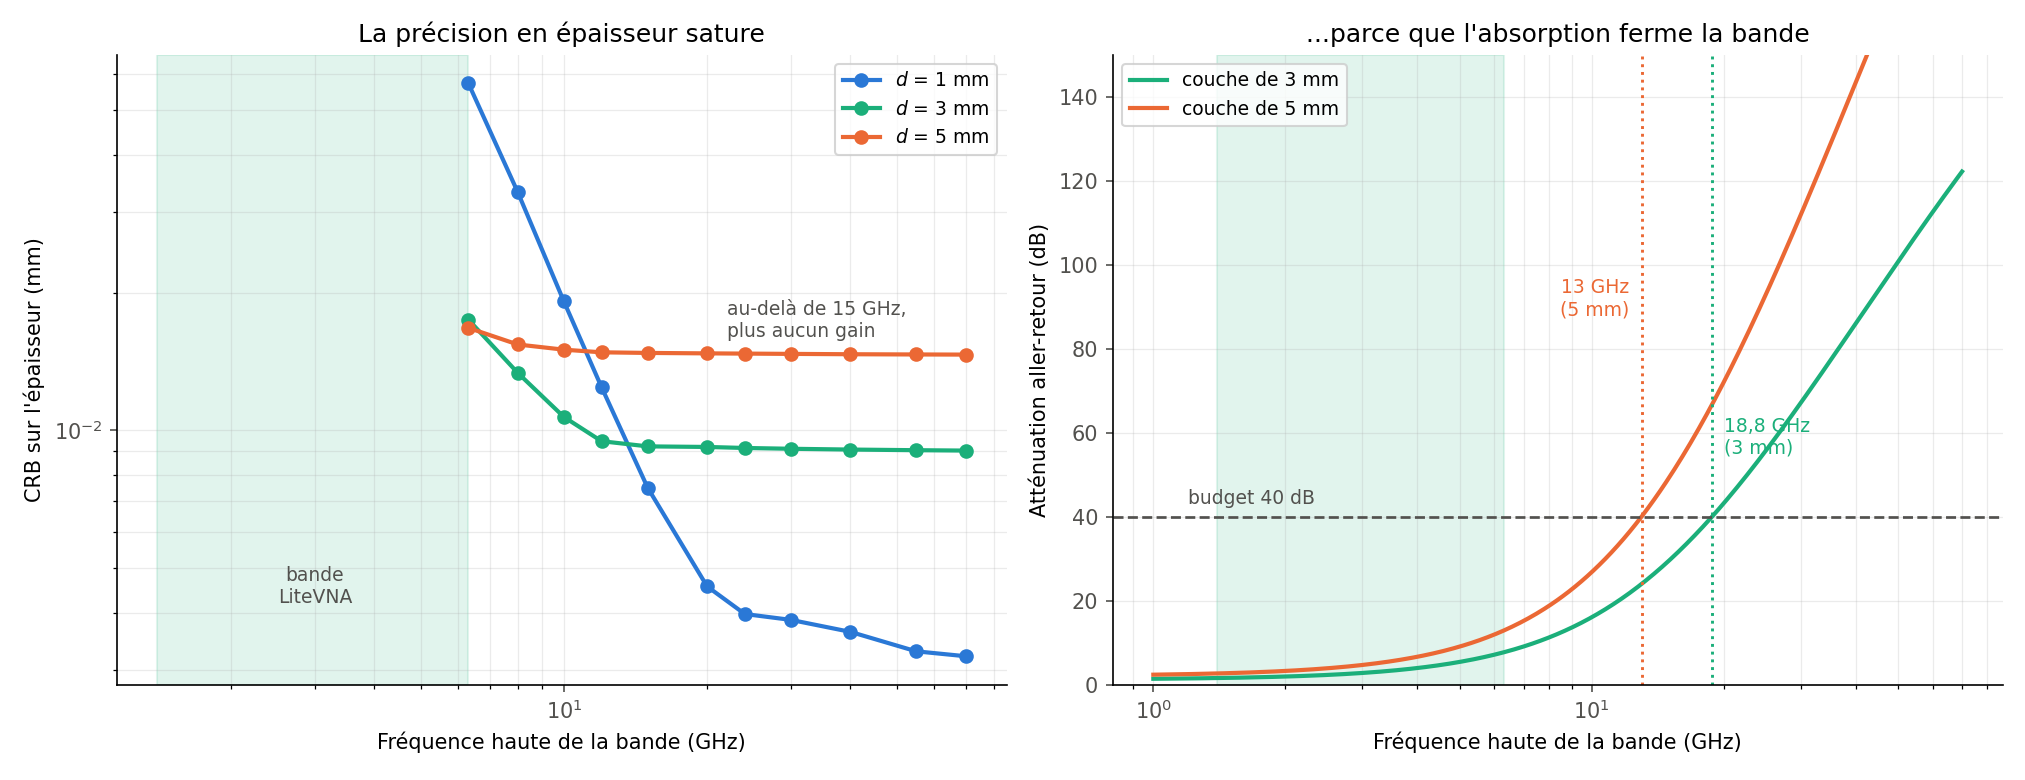
\includegraphics[width=\textwidth]{fig_saturation_bande.png}
\end{center}

À $5$~mm d'épaisseur, la précision vaut $0{,}015$~mm de $10$ à $70$~GHz :
identique. Passer de $8{,}6$ à $68{,}6$~GHz de bande n'apporte rigoureusement
rien, parce que toute fréquence au-dessus de $15$~GHz porte une information de
Fisher nulle sur $d$. À temps de mesure constant, c'est même défavorable
($0{,}017 \to 0{,}055$~mm) : élargir la bande à nombre de points fixe dilue
l'échantillonnage de la portion utile.

\begin{implication}
La seule raison valable de monter en fréquence est la \textbf{résolution
latérale} (\S\ref{sec:lateral}), et l'optimum se situe alors vers $15$~GHz.
Monter pour améliorer la résolution en épaisseur est sans objet. Et aucun
instrument ne remplace la connaissance de $\eps$ : à $3$~mm, la caractériser
fait passer de $0{,}170$ à $0{,}017$~mm --- un facteur $10$ que même $70$~GHz
n'approche pas.
\end{implication}

%=======================================================================
\section{La distance antenne--objet}
\label{sec:standoff}
%=======================================================================

\subsection{Elle n'est pas une entrée de la mesure}

L'épaisseur se lit dans la \emph{forme} des franges d'interférence de
$\Gamma(f)$, non dans un retard absolu. Le retard de standoff $\tau_0$ est donc
un paramètre libre, ajusté conjointement à $d$. Coût de son ignorance, CRB à
$100$~mm :

\begin{table}[h]
\centering
\begin{tabular}{lccc}
\toprule
$d$ & distance connue & distance inconnue & coût \\
\midrule
$1$~mm & $0{,}019$~mm  & $0{,}057$~mm  & $\times 2{,}97$ \\
$3$~mm & $0{,}0174$~mm & $0{,}0175$~mm & $\times 1{,}00$ \\
$5$~mm & $0{,}0162$~mm & $0{,}0167$~mm & $\times 1{,}04$ \\
\bottomrule
\end{tabular}
\end{table}

Pour le cartilage épais, l'ignorer ne coûte rien : \textbf{la mesure est
auto-référencée}. Seule la couche mince paie un facteur $3$, parce qu'elle agit
presque comme un retard pur et devient partiellement dégénérée avec $\tau_0$.

\subsection{Quatre exigences distinctes}

\paragraph{Stabilité pendant le balayage.} Un déplacement $e$ pendant les
$0{,}25$~s d'acquisition crée une erreur de phase $4\pi e/\lambda$,
indiscernable d'un changement d'épaisseur. À $6{,}3$~GHz, les $0{,}25^\circ$ de
bruit de phase mesuré correspondent à $e = 16{,}5\,\mu$m. \textbf{Le robot doit
être à l'arrêt pendant la mesure} : arrêt--mesure--marche, jamais de balayage
continu. C'est la plus dure des quatre contraintes.

\paragraph{Distance minimale.} L'écho d'antenne doit être séparable de l'écho de
surface. Le lobe principal vaut $\simeq 1{,}7\,c/2B$, soit $52$~mm en bande
complète : le standoff devrait dépasser $78$~mm. En bande réduite
$3$--$6{,}3$~GHz le lobe atteint $77$~mm et la borne monte à $116$~mm.
Travailler à $20$~mm reste possible, mais impose alors de \emph{soustraire}
vectoriellement la réflexion propre de l'antenne plutôt que de la séparer
temporellement.

\paragraph{Distance maximale.} Le rapport signal à bruit s'effondre en $1/R^2$
(réflecteur plan) à $1/R^4$ (surface fortement courbée) :

\begin{table}[h]
\centering
\caption{CRB sur $d$ (mm), distance inconnue, $\eps$ connu.}
\begin{tabular}{lcccc}
\toprule
$R$ & plan, $1$~mm & plan, $3$~mm & courbe, $1$~mm & courbe, $3$~mm \\
\midrule
$100$~mm & $0{,}057$ & $0{,}017$ & $0{,}057$ & $0{,}017$ \\
$150$~mm & $0{,}086$ & $0{,}026$ & $0{,}129$ & $0{,}039$ \\
$200$~mm & $0{,}115$ & $0{,}035$ & $0{,}229$ & $0{,}070$ \\
$300$~mm & $0{,}172$ & $0{,}052$ & $0{,}516$ & $0{,}157$ \\
\bottomrule
\end{tabular}
\end{table}

À $500$~mm il manque $13$~dB de rapport signal à bruit pour tenir $0{,}1$~mm sur
une surface courbée, et $23$~dB pour une couche de $1$~mm.

\paragraph{Courbure du front d'onde.} Le modèle suppose une onde plane à
l'interface. La flèche de la sphère d'onde sur une empreinte de largeur $w$ vaut
$w^2/8R$, à comparer à $\lambda/16$ ($2{,}97$~mm à $6{,}3$~GHz). À $100$~mm avec
une empreinte de $30$~mm : $1{,}12$~mm, confortable. À $20$~mm, la même empreinte
donne $5{,}6$~mm : \textbf{l'empreinte doit alors rester sous $10$~mm}, ce qui
contraint l'antenne à être petite.

\subsection{La fenêtre utile}

Bornée en bas par la séparation de l'écho d'antenne et la courbure du front
d'onde, en haut par le rapport signal à bruit sur le cas contraignant --- couche
mince sur condyle courbé --- la fenêtre s'établit à $100$--$150$~mm en régime de
temps de vol, et descend à $20$--$30$~mm si l'on accepte la soustraction
vectorielle de la réflexion d'antenne. C'est exactement la plage codée dans
\texttt{qualification.py}, désormais justifiée plutôt que devinée.

\subsection{Une synergie avec le relevé optique}

Le système optique fournit la surface externe, donc le standoff. L'imposer au
lieu de le laisser libre produit le biais suivant, selon l'erreur optique
$\delta R$ :

\begin{table}[h]
\centering
\begin{tabular}{lccc}
\toprule
$\delta R$ & $d = 1$~mm & $3$~mm & $5$~mm \\
\midrule
$0{,}05$~mm & $-0{,}031$ & $+0{,}002$ & $+0{,}008$ \\
$0{,}10$~mm & $-0{,}062$ & $+0{,}005$ & $+0{,}016$ \\
$0{,}20$~mm & $-0{,}121$ & $+0{,}011$ & $+0{,}031$ \\
$0{,}50$~mm & $-0{,}273$ & $+0{,}034$ & $+0{,}072$ \\
\bottomrule
\end{tabular}
\end{table}

\begin{implication}
Imposer le standoff optique n'est gagnant que si la reconstruction optique est
meilleure que $0{,}1$~mm, et seulement sur le cartilage mince --- à comparer aux
$0{,}057 / 0{,}017 / 0{,}017$~mm obtenus en laissant la distance libre. Au-delà,
on injecte plus d'erreur qu'on n'en retire. Pour le cartilage épais, laisser
libre : c'est gratuit.
\end{implication}

%=======================================================================
\section{La calibration vectorielle}
\label{sec:cal}
%=======================================================================

\subsection{Pourquoi le menu du LiteVNA ne suffit pas}

Le LiteVNA possède un menu \textsc{cal} qui réalise bien une calibration SOL et
réclame bien les mêmes étalons physiques. Mais \textbf{son interface USB renvoie
toujours des données brutes, par conception} : la calibration effectuée sur
l'appareil ne corrige que son propre écran. Ce choix est délibéré et documenté
--- il évite toute ambiguïté sur la nature des données transmises et laisse
l'hôte appliquer des routines supérieures. Tout ce que lit
\texttt{get\_s11\_s21()} est donc non corrigé, quelle que soit la calibration
présente dans l'instrument.

\subsection{Le modèle d'erreur à un port}

\begin{equation}
\Gamma_{\text{mes}} = e_{00}
  + \frac{e_{10}e_{01}\,\Gamma_{\text{vrai}}}{1 - e_{11}\,\Gamma_{\text{vrai}}}
\label{eq:oneport}
\end{equation}

où $e_{00}$ est la \emph{directivité} --- le signal qui fuit du pont vers le
récepteur sans jamais atteindre l'antenne, et qui crée le faux écho à distance
nulle ; $e_{11}$ la \emph{désadaptation source}, responsable des allers-retours
entre le VNA et une antenne mal adaptée ($-6{,}6$~dB dans notre bande haute,
soit $22\,\%$ réfléchi) ; et $e_{10}e_{01}$ le \emph{suivi en réflexion}.
L'inversion donne

\begin{equation}
\Gamma_{\text{vrai}} = \frac{\Gamma_{\text{mes}} - e_{00}}
     {e_{10}e_{01} + e_{11}\,(\Gamma_{\text{mes}} - e_{00})}
\end{equation}

En pratique on résout le système sous forme bilinéaire, linéaire en les
inconnues et numériquement bien mieux conditionnée : en posant $d = e_{00}$,
$s = e_{11}$ et $t = e_{10}e_{01} - e_{00}e_{11}$,
$\Gamma_m = d + s\,(\Gamma_a\Gamma_m) + t\,\Gamma_a$, soit un système
$3\times3$ exact à chaque fréquence.

\subsection{Faut-il des étalons caractérisés ?}

Un kit générique ne publie pas ses coefficients. Simulation de la chaîne
complète --- mesure, calibration avec des étalons \emph{supposés} idéaux,
inversion par le modèle physique avec retard et gain complexe libres :

\begin{table}[h]
\centering
\caption{Biais sur l'épaisseur, couche de $1$ à $5$~mm.}
\begin{tabular}{ll}
\toprule
Défaut du kit ignoré & Biais maximal \\
\midrule
Ouvert, $20$ à $100$~fF        & $0{,}01$ à $0{,}04$~mm \quad négligeable \\
Offsets de $5$~ps              & $0{,}03$~mm \quad négligeable \\
Court-circuit, $0{,}10$~nH     & $0{,}07$~mm \quad acceptable \\
Court-circuit, $0{,}30$~nH     & $0{,}98$~mm \quad \textbf{rédhibitoire} \\
Charge à $-25$~dB au lieu de $-45$ & $1{,}24$~mm \quad \textbf{rédhibitoire} \\
\bottomrule
\end{tabular}
\end{table}

L'ordre d'importance est \textbf{charge $\gg$ court-circuit $\gg$ ouvert}, et
non l'inverse comme on le suppose souvent. La raison : tout ce qui est linéaire
en fréquence --- capacité de frange de l'ouvert, offsets --- est absorbé par le
réglage du plan de référence sur plaque métallique ; seule la courbure subsiste.
L'inductance du court-circuit et surtout la réflexion résiduelle de la charge ne
le sont pas : elles se logent dans la directivité, précisément là où vit l'écho
de fond de couche.

\begin{implication}
La charge $50\,\Omega$ est la pièce critique du kit. Elle fixe le plancher de
mesure, et c'est elle qu'il faut remplacer si le plancher mesuré est médiocre.
Le module \texttt{calibration.py} implante l'acquisition guidée, la
résolution, la sauvegarde des termes d'erreur et un mode de vérification qui
mesure ce plancher. Conserver les balayages bruts permet de recalibrer plus tard
avec de meilleurs modèles d'étalons --- ce que la calibration embarquée, qui
détruit l'information à l'acquisition, interdit.
\end{implication}

%=======================================================================
\section{Faisabilité avec le LiteVNA}
%=======================================================================

\subsection{Ce que l'instrument sait faire : mesures sur notre banc}

Toutes les valeurs ci-dessous ont été mesurées, non extrapolées ---
$48$~balayages répartis en trois campagnes indépendantes.

\begin{table}[h]
\centering
\renewcommand{\arraystretch}{1.2}
\begin{tabular}{p{4.3cm}p{3.4cm}p{6.2cm}}
\toprule
Grandeur & Mesuré & Verdict \\
\midrule
Bande utile & $1{,}4$--$6{,}3$~GHz & meilleur que tout module UWB du commerce \\
Bruit de phase, balayage à balayage & $0{,}23$ à $0{,}42^{\circ}$ & excellent \\
Cohérence & $\geq 0{,}9997$ & moyennage vectoriel quasi parfait \\
Gigue de position d'un écho & $0{,}008$~mm & $6\,600$ fois sous la résolution \\
Dérive entre campagnes & $7\,\%$ / $2{,}7^{\circ}$ (médiane)
  & bornée, non cumulative \\
Nature de la dérive & $<6\,\%$ expliqué par une rampe
  & décorrélée $\Rightarrow$ se moyenne \\
Débit & $\simeq 0{,}25$~s par balayage de $101$ points & suffisant (\S\ref{sec:sar}) \\
\bottomrule
\end{tabular}
\end{table}

\begin{center}
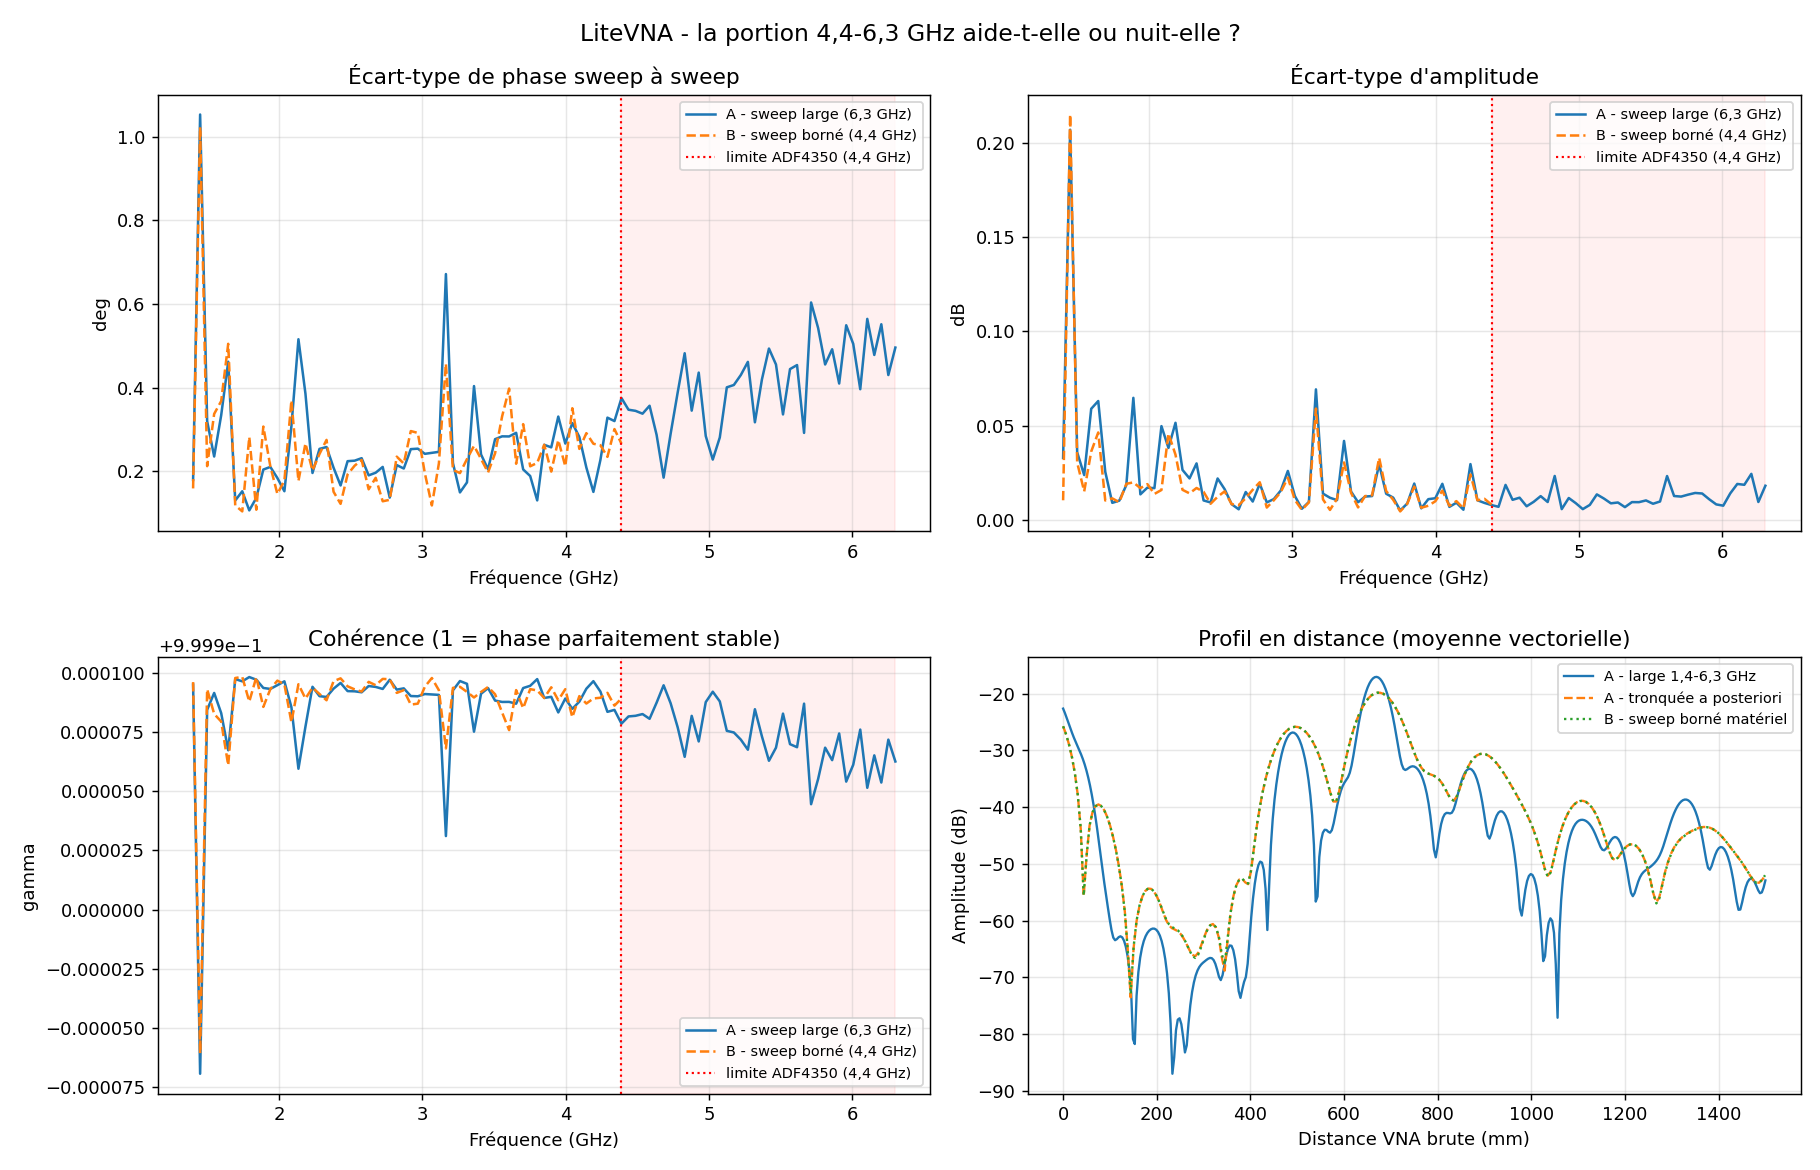
\includegraphics[width=0.92\textwidth]{comparaison_bande.png}
\end{center}

Un test dédié a par ailleurs établi qu'il faut \textbf{conserver toute la bande}
$1{,}4$--$6{,}3$~GHz : borner le balayage à $4{,}4$~GHz n'assainit pas le bas de
bande (rapport $0{,}93$ / $0{,}97$ / $0{,}98$ sur trois campagnes) et dégrade la
gigue d'un facteur~$3$. Le haut de bande est $1{,}5$ à $1{,}8$~fois plus bruité,
mais cet excès est négligeable en valeur absolue.

\subsection{Les limites réelles}

\begin{enumerate}
\item \textbf{Absence de déclenchement matériel.} Le LiteVNA ne dispose
      d'aucune entrée de synchronisation. L'appariement entre une pose du robot
      et un balayage ne peut donc se faire qu'en mode \emph{arrêt--mesure--
      marche} piloté par logiciel. C'est la limitation la plus structurante pour
      un banc robotisé : elle interdit le balayage en mouvement continu et fixe
      le débit à environ une pose par seconde.
\item \textbf{Pas de calibration SOL dans le micrologiciel.} L'appareil renvoie
      des données non corrigées. Toute la correction d'erreurs doit être
      implantée côté logiciel, avec des étalons Short/Open/Load ramenés au plan
      de l'antenne.
\item \textbf{Dynamique en haut de bande.} L'écho de fond se situe
      $14{,}5$~dB sous l'écho de surface, et le mélangeur unique commuté du
      LiteVNA voit sa dynamique se dégrader au-dessus de $6$~GHz. La marge
      existe mais elle n'est pas confortable.
\item \textbf{Antenne actuelle inadaptée.} $|S_{11}| = -6{,}6$~dB entre $4{,}2$
      et $4{,}9$~GHz, c'est-à-dire $22\,\%$ de puissance réfléchie en pure
      perte, précisément dans la portion de bande la plus informative
      (\S\ref{sec:hautbande}).
\item \textbf{Aucune qualification médicale.} L'appareil n'est ni certifiable ni
      stérilisable ; il ne peut servir qu'à la démonstration de principe.
\end{enumerate}

\subsection{Verdict}

\begin{center}
\fbox{\begin{minipage}{0.92\textwidth}
\textbf{Le LiteVNA est adapté à la démonstration de faisabilité, et inadapté à
un système clinique.}\\[1mm]
Il possède la bande passante, la stabilité de phase et le débit nécessaires ---
tous mesurés. Il lui manque le déclenchement matériel, la calibration
vectorielle et la qualification. Le facteur limitant du projet n'est ni
l'instrument, ni la bande : c'est la stabilité mécanique du montage, puis la
connaissance de $\eps$.
\end{minipage}}
\end{center}

\subsection{Étape suivante pour un banc robotisé}

Pour la phase robotisée, une plateforme ouverte de type LibreVNA
($100$~kHz--$6$~GHz, deux récepteurs indépendants, synthétiseur MAX2871,
matériel et micrologiciel ouverts, pilotage SCPI documenté) présente un avantage
décisif : \textbf{elle est scriptable et modifiable}, donc synchronisable avec
le robot, et sa calibration vectorielle est déjà implantée.

Il faut souligner que cet argument est celui de l'\emph{intégration}, non celui
de la qualité de mesure : nos mesures montrent que le mélangeur commuté du
LiteVNA ne pose aucun problème observable à court terme, et l'hypothèse selon
laquelle deux récepteurs simultanés amélioreraient la phase n'est pas confirmée
par les données.

Cette recommandation vaut pour la phase de démonstration. Pour un dispositif
clinique, l'architecture pertinente n'est plus un VNA mais un radar FMCW, qui
lève les deux mêmes limitations d'un facteur bien supérieur
(\S\ref{sec:fmcw}).

%=======================================================================
\section{Une alternative : le radar FMCW}
\label{sec:fmcw}
%=======================================================================

\subsection{C'est la même mesure}

Un VNA en balayage pas-à-pas et un radar à modulation de fréquence continue
(FMCW) échantillonnent tous deux le coefficient de réflexion complexe
$\Gamma(f)$ sur une bande. Le premier s'arrête à chaque fréquence ; le second
balaie en rampe continue et démodule le signal reçu par le signal émis
(\emph{deramping}), ce qui transforme le retard $\tau$ en une fréquence de
battement $f_b = (B/T)\,\tau$. Pour une scène statique,
\textbf{l'information est identique}.

Tout ce qui précède se transpose donc sans modification : résolution axiale
$c/2B$, borne de Cramér--Rao sur $d$, plafond d'absorption de $13$ à $19$~GHz
(\S\ref{sec:bande}), résolution latérale $\lambda/4$ (\S\ref{sec:lateral}),
inversion sur modèle stratifié, rétroprojection (\S\ref{sec:sar}). Le FMCW ne
change rien à la physique. Il change le \emph{budget de mouvement}, et cela
suffit à en faire l'architecture du produit.

\subsection{UWB et FMCW ne sont pas sur le même axe}
\label{sec:uwbfmcw}

Les deux termes ne s'opposent pas : \textbf{UWB} est un critère de \emph{largeur
de bande} --- et une catégorie réglementaire --- tandis que \textbf{FMCW} est un
choix de \emph{forme d'onde}. Le critère UWB (FCC, ETSI) est
$B \ge 500$~MHz \emph{ou} $B/f_c \ge 20\,\%$.

\begin{table}[h]
\centering
\begin{tabular}{lcccc}
\toprule
Système & $B$ & $f_c$ & $B/f_c$ & UWB ? \\
\midrule
\textbf{LiteVNA $1{,}4$--$6{,}3$~GHz} & $4{,}90$~GHz & $3{,}85$~GHz
  & $\mathbf{127\,\%}$ & oui \\
FMCW $3{,}1$--$10{,}6$~GHz & $7{,}50$~GHz & $6{,}85$~GHz & $109\,\%$ & oui \\
IR-UWB type $6{,}6$--$8{,}0$ & $1{,}40$~GHz & $7{,}30$~GHz & $19\,\%$ & oui \\
FMCW automobile $77$--$81$ & $4{,}00$~GHz & $79$~GHz & $5\,\%$ & oui \\
ISM $24{,}0$--$24{,}25$ & $0{,}25$~GHz & $24{,}1$~GHz & $1\,\%$ & non \\
\bottomrule
\end{tabular}
\end{table}

Notre instrument est donc \emph{déjà} un radar UWB, et l'un des plus larges qui
soient. L'étiquette renseigne d'ailleurs peu : un chirp automobile à $5\,\%$ de
bande fractionnaire la porte au même titre.

Dans l'usage courant, « radar UWB » désigne plus étroitement le radar
\emph{impulsionnel} (IR-UWB), qui émet une impulsion brève et échantillonne
l'écho directement dans le temps. C'est alors une troisième forme d'onde, à côté
du FMCW et du pas-à-pas.

\paragraph{Les trois mesurent la même chose.} Toutes caractérisent la réponse
impulsionnelle $h(t)$, ou de façon équivalente $\Gamma(f)$. Elles ne diffèrent
que par la manière de répartir l'énergie dans le temps.

\begin{table}[h]
\centering
\begin{tabular}{lccc}
\toprule
& Impulsionnel & FMCW & Pas-à-pas \\
\midrule
Domaine natif & temps & battement & fréquence \\
Énergie & concentrée en $204$~ps & étalée sur $100\,\mu$s & $N$ paliers \\
Facteur de crête & $27$ à $37$~dB & $\mathbf{0}$~\textbf{dB} & $0$~dB \\
Convertisseur & $9{,}8$~GSa/s & $\mathbf{0{,}33}$~\textbf{MSa/s} & lent \\
\bottomrule
\end{tabular}
\end{table}

Pour $B = 4{,}9$~GHz, l'impulsion équivalente dure $1/B = 204$~ps, soit $61$~mm
dans l'air. Le FMCW obtient la même résolution en étalant cette énergie sur le
chirp : le produit $B\!\cdot\!T = 4{,}9\times10^5$ donne
\textbf{$56{,}9$~dB de gain de compression d'impulsion}. Autrement dit, le FMCW
délivre la résolution d'une impulsion de $204$~ps avec la puissance crête d'un
émetteur continu --- et un convertisseur trente mille fois plus lent.
L'échantillonnage en temps équivalent, employé par l'IR-UWB pour contourner les
$9{,}8$~GSa/s, exige un tir par point de retard : le temps d'acquisition total
redevient comparable à celui d'un chirp, \emph{sans} le gain de compression.

\begin{implication}
« UWB » ne désigne pas une technologie concurrente du FMCW : notre système
l'est déjà. Le seul vrai choix est celui de la forme d'onde, et il se tranche
sur la puissance crête et le convertisseur --- deux postes où le FMCW gagne de
plusieurs ordres de grandeur.
\end{implication}

\subsection{L'avantage décisif : le balayage continu}

La contrainte la plus dure identifiée jusqu'ici est celle des $15\,\mu$m de
déplacement tolérés pendant une acquisition (\S\ref{sec:standoff}).

\begin{table}[h]
\centering
\begin{tabular}{lcc}
\toprule
Acquisition & Durée & Vitesse robot maximale \\
\midrule
LiteVNA, $101$ points & $250$~ms & $0{,}06$~mm/s \\
Chirp FMCW & $100\,\mu$s & $\mathbf{150}$~\textbf{mm/s} \\
Chirp FMCW rapide & $10\,\mu$s & $1\,500$~mm/s \\
\bottomrule
\end{tabular}
\end{table}

Le facteur $2\,500$ fait basculer le mode opératoire de
l'arrêt--mesure--marche vers le \textbf{balayage continu}, et le bénéfice se
compose :

\begin{itemize}
\item à $150$~mm/s avec un cycle de $200\,\mu$s, le déplacement entre deux
      chirps vaut $30\,\mu$m, alors que l'échantillonnage de l'ouverture
      synthétique n'en exige qu'un tous les $\lambda/4 = 11{,}9$~mm ;
\item il tombe donc \textbf{$397$ chirps dans chaque cellule
      d'échantillonnage}, soit $26$~dB de moyennage \emph{gratuit} ;
\item une zone de $100 \times 80$~mm se balaie en $5{,}3$~s au lieu de $60$~s.
\end{itemize}

\subsection{Deux avantages structurels}

\paragraph{La corrélation de portée annule le bruit de phase.} Le signal reçu
est démodulé par une réplique de lui-même retardée de $\tau$ seulement : le
bruit de phase de l'oscillateur se soustrait à lui-même. Le résidu vaut
$S(f)\,4\sin^2(\pi f\tau) \simeq S(f)\,(2\pi f\tau)^2$.

\begin{table}[h]
\centering
\begin{tabular}{lcc}
\toprule
Distance & $f_b$ & Suppression du bruit de phase \\
\midrule
$20$~mm  & $6{,}5$~kHz & $-105$~dB \\
$100$~mm & $32{,}7$~kHz & $-77$~dB \\
$500$~mm & $163$~kHz & $-49$~dB \\
\bottomrule
\end{tabular}
\end{table}

À nos distances, le bruit de phase de l'oscillateur \textbf{disparaît du budget
d'erreur}. C'est un avantage intrinsèque du FMCW à courte portée.

\paragraph{La linéarité de rampe n'est pas contraignante.} L'épaisseur étant un
\emph{écart} de retards, une erreur relative de pente se reporte en erreur
relative sur $d$ : $0{,}1\,\%$ de non-linéarité donne $0{,}003$~mm à $3$~mm et
$0{,}005$~mm à $5$~mm d'épaisseur. Une boucle à verrouillage de phase atteint
couramment $0{,}01\,\%$.

La numérisation est également modeste : les battements valent $6{,}5$ à
$49$~kHz sur la fenêtre $20$--$150$~mm, et $2$~MSa/s avec $200$~échantillons par
chirp suffisent à couvrir une portée non ambiguë de $3$~m --- soit exactement le
rôle que jouent les $201$ points du VNA.

\subsection{Le blocage : aucun composant du commerce n'est à la bonne bande}

\begin{table}[h]
\centering
\caption{Bandes candidates. Résolution latérale à $R = 20$~mm, $L = 100$~mm.}
\begin{tabular}{lcccll}
\toprule
Bande & $B$ & Latéral & Att. $3$~mm & Att. $5$~mm & Composants \\
\midrule
$1{,}4$--$6{,}3$~GHz & $4{,}9$~GHz & $12{,}8$~mm & $8$~dB & $13$~dB
  & sur mesure \\
$3{,}1$--$10{,}6$~GHz & $7{,}5$~GHz & $7{,}6$~mm & $18$~dB & $29$~dB
  & sur mesure \\
$1{,}4$--$15$~GHz & $13{,}6$~GHz & $5{,}4$~mm & $30$~dB & $49$~dB
  & sur mesure \\
$57$--$64$~GHz & $7{,}0$~GHz & $1{,}3$~mm & $117$~dB & $194$~dB
  & intégrés \\
$77$--$81$~GHz & $4{,}0$~GHz & $1{,}0$~mm & $131$~dB & $218$~dB
  & intégrés \\
\bottomrule
\end{tabular}
\end{table}

Le piège est lisible d'un coup d'\oe il : les deux seules bandes où des circuits
FMCW intégrés existent offrent une résolution latérale superbe --- et une
atténuation de $120$ à $220$~dB. Le tissu y est parfaitement opaque. Les bandes
utiles réclament toutes une conception radiofréquence spécifique : boucle à
rampe, oscillateur commandé large bande (couvrir $3{,}1$--$10{,}6$~GHz
représente un rapport $3{,}4{:}1$, généralement obtenu par plusieurs
oscillateurs commutés), mélangeur de démodulation et chaîne bas bruit.

\subsection{La contrainte réglementaire, et ce qu'elle change}
\label{sec:reglementaire}

Le masque UWB ($-41{,}3$~dBm/MHz PIRE) ne couvre que $3{,}1$ à $10{,}6$~GHz.
Notre bande $1{,}4$--$6{,}3$~GHz en déborde de $1{,}7$~GHz par le bas, dans des
portions attribuées à des services existants. Sur un banc de laboratoire à
faible puissance, c'est sans conséquence ; pour un \emph{dispositif}, c'est un
obstacle qui n'apparaissait nulle part dans l'analyse physique.

\begin{table}[h]
\centering
\begin{tabular}{lll}
\toprule
Portion & Largeur & Statut \\
\midrule
$1{,}4$--$3{,}1$~GHz & $1{,}70$~GHz & \textbf{hors masque UWB} \\
$3{,}1$--$6{,}3$~GHz & $3{,}20$~GHz & UWB, mitigation requise en UE \\
$\mathbf{6{,}0}$--$\mathbf{8{,}5}$~\textbf{GHz} & $2{,}50$~GHz
  & \textbf{UWB, sous-bande la plus propre en UE} \\
$8{,}5$--$10{,}6$~GHz & $2{,}10$~GHz & UWB, restrictions selon zone \\
\bottomrule
\end{tabular}
\end{table}

La sous-bande la plus simple à faire accepter en Europe ne fait que la moitié de
la bande actuelle. Or elle suffit :

\begin{table}[h]
\centering
\begin{tabular}{lcc}
\toprule
& $1{,}4$--$6{,}3$~GHz & $\mathbf{6{,}0}$--$\mathbf{8{,}5}$~\textbf{GHz} \\
\midrule
CRB à $1/3/5$~mm & $0{,}057 / 0{,}017 / 0{,}017$~mm
                 & $0{,}067 / 0{,}017 / 0{,}041$~mm \\
Résolution latérale ($R=20$, $L=100$) & $12{,}8$~mm
                                      & $\mathbf{9{,}5}$~\textbf{mm} \\
Atténuation $3/5$~mm & $8 / 13$~dB & $12 / 21$~dB \\
Statut réglementaire & non conforme & \textbf{conforme sans mitigation} \\
\bottomrule
\end{tabular}
\end{table}

Elle tient la spécification des $0{,}1$~mm, \emph{améliore} la résolution
latérale de $26\,\%$, et elle est légale. C'est une confirmation directe de la
thèse centrale de ces notes : on n'a jamais eu besoin de résolution, seulement
de sensibilité --- perdre la moitié de la bande ne coûte donc presque rien.

\emph{Ces valeurs sont un ordre de grandeur réglementaire et non un avis de
conformité : les sous-bandes et les obligations de mitigation évoluent, et il
faut les vérifier contre la version en vigueur d'ETSI EN 302 065.}

\subsection{Spécification}

\begin{table}[h]
\centering
\begin{tabular}{lll}
\toprule
Paramètre & Valeur & Origine \\
\midrule
Bande & $6{,}0$--$8{,}5$~GHz & sous-bande UWB propre en UE
  (\S\ref{sec:reglementaire}) \\
Excursion & $\ge 2{,}5$~GHz & suffisante : CRB $0{,}017$~mm à $3$~mm \\
Durée de chirp & $100\,\mu$s & budget $15\,\mu$m $\to$ $150$~mm/s \\
Pente & $25$~THz/s & $B/T$ \\
Linéarité & $< 0{,}1\,\%$ & $0{,}005$~mm à $5$~mm \\
Cadence & $\ge 5\,000$ chirps/s & moyennage SAR gratuit \\
Convertisseur & $2$~MSa/s, $14$--$16$ bits & $200$ éch./chirp \\
Isolation TX/RX & $\ge 40$~dB & fuite au battement de la cible \\
Dynamique & $\ge 60$~dB & écho de fond à $-17$~dB + marge \\
Ouverture d'antenne & $\le 10$~mm & courbure du front d'onde à $20$~mm \\
\textbf{Sortie exigée} & $\Gamma(f)$ complexe calibré & l'inversion
  exige la phase \\
\bottomrule
\end{tabular}
\end{table}

La dernière ligne est la plus facile à omettre : la plupart des
environnements de développement de radars FMCW livrent un \emph{profil de
distance en module}. L'inversion sur modèle stratifié exige le spectre complexe,
avec la calibration du \S\ref{sec:cal} appliquée dessus. C'est une exigence de
conception, non un choix de composant.

Un point de cohérence confirme le cadre : la résolution en battement vaut
$1/T = 10$~kHz alors qu'une cible à $20$~mm se situe à $6{,}5$~kHz. La fuite
entre émission et réception et l'écho de cible tombent donc dans la même
cellule --- exactement le recouvrement avec l'écho d'antenne déjà rencontré à
$20$~mm pour le VNA (\S\ref{sec:standoff}), et pour la même raison
($c/2B = 30{,}6$~mm $> 20$~mm). Les deux technologies héritent de la contrainte
à l'identique, et la parade est la même : soustraction vectorielle du fond.

\subsection{Bilan de liaison}
\label{sec:bilan}

La spécification précédente est-elle réalisable sous le plafond réglementaire ?
Le masque UWB impose $-41{,}3$~dBm/MHz de PIRE, soit sur $2\,500$~MHz un total
de $-7{,}3$~dBm --- \textbf{$0{,}19$~mW}. C'est un plafond légal, non une
performance à acheter : le bilan doit donc tenir avec cette seule puissance.

\begin{table}[h]
\centering
\caption{Bilan de liaison, standoff $20$~mm, bande $6{,}0$--$8{,}5$~GHz.}
\begin{tabular}{lrl}
\toprule
Poste & Valeur & Origine \\
\midrule
PIRE émise & $-7{,}3$~dBm & plafond UWB sur $2{,}5$~GHz \\
Couplage aller-retour à $20$~mm & $-6{,}0$~dB & \emph{hypothèse} \\
Pertes de chaîne & $-8{,}0$~dB & \emph{hypothèse} : antenne,
  circulateur, connectique \\
Réflexion de surface $r_{12}$ & $-2{,}6$~dB & Fresnel air/cartilage \\
\midrule
\textbf{Écho de surface reçu} & $\mathbf{-23{,}9}$~\textbf{dBm} & \\
\midrule
Écho de fond / surface & $-13{,}6$~dB & $(1-r_{12}^2)\,r_{23}/r_{12}$ \\
Absorption aller-retour, $3$~mm & $-12{,}5$~dB & modèle de Debye
  (\S\ref{sec:debye}) \\
\textbf{Écho de fond reçu, $3$~mm} & $\mathbf{-50{,}0}$~\textbf{dBm} & \\
Absorption aller-retour, $5$~mm & $-20{,}8$~dB & \\
\textbf{Écho de fond reçu, $5$~mm} & $\mathbf{-58{,}3}$~\textbf{dBm} & \\
\midrule
Plancher de bruit & $-128{,}0$~dBm
  & $-174 + \mathrm{NF} + 10\log_{10}(1/T)$ \\
\bottomrule
\end{tabular}
\end{table}

Le plancher mérite un mot, car c'est l'étape la moins intuitive. Après
démodulation, le signal d'une cellule de distance donnée n'occupe qu'une
largeur $1/T = 10$~kHz : \emph{c'est elle, et non les $2{,}5$~GHz de la bande
émise, qui fixe la bande de bruit}. Avec un facteur de bruit de $6$~dB, le
plancher vaut donc $-174 + 6 + 40 = -128$~dBm.

\begin{table}[h]
\centering
\begin{tabular}{lcc}
\toprule
& Couche de $3$~mm & Couche de $5$~mm \\
\midrule
RSB par rampe & $+78$~dB & $\mathbf{+70}$~\textbf{dB} \\
RSB après moyennage SAR ($397$ rampes) & $+104$~dB & $+96$~dB \\
\bottomrule
\end{tabular}
\end{table}

Soixante-dix décibels sur le cas le plus défavorable --- cartilage de $5$~mm, à
la puissance légale maximale. Les deux postes marqués « hypothèse » sont les
plus fragiles du calcul, mais la marge les absorbe largement : même en ajoutant
$30$~dB de pertes non modélisées, il resterait $40$~dB de rapport signal à
bruit.

\begin{implication}
Ce résultat valide rétrospectivement l'hypothèse de $30$~dB utilisée depuis le
début de ces notes pour toutes les bornes de Cramér--Rao : elle était
conservatrice. Il établit surtout que \textbf{la contrainte de puissance UWB
n'est pas un obstacle} --- ce qui fixe le plancher réel n'est pas la puissance
émise mais la directivité résiduelle après calibration (\S\ref{sec:cal}). Le
poste critique du budget n'est pas l'émetteur : c'est la charge $50\,\Omega$ du
kit d'étalons.
\end{implication}

\subsection{L'offre du marché}
\label{sec:marche}

Aucun module du commerce ne satisfait cette spécification. Les circuits FMCW
intégrés existants sont tous en ondes millimétriques ($24$, $60$, $77$~GHz), où
le tissu est opaque. Dans la bande UWB autorisée, l'offre est
\emph{impulsionnelle} et étroite :

\begin{table}[h]
\centering
\caption{CRB sur l'épaisseur (mm) des modules disponibles. Objectif
$0{,}100$~mm.}
\begin{tabular}{llccccl}
\toprule
Produit & Bande & $B$ & $1$~mm & $3$~mm & $5$~mm & \\
\midrule
LiteVNA (référence) & $1{,}4$--$6{,}3$ & $4{,}90$~GHz
  & $0{,}057$ & $0{,}017$ & $0{,}017$ & --- \\
Vayyar VYYR2401 (UE) & $6{,}3$--$8{,}0$ & $1{,}70$~GHz
  & $0{,}099$ & $0{,}023$ & $0{,}053$ & limite \\
Novelda X7F202 & $7{,}5$--$8{,}25$ & $0{,}75$~GHz
  & $0{,}218$ & $0{,}064$ & $0{,}502$ & insuffisant \\
TDSR P452 & $4{,}0$--$4{,}6$ & $0{,}60$~GHz
  & $0{,}448$ & $0{,}120$ & $0{,}039$ & insuffisant \\
\bottomrule
\end{tabular}
\end{table}

Un seul candidat approche la cible, et sans marge : le VYYR2401 de Vayyar, dont
la variante européenne couvre $6{,}3$--$8{,}0$~GHz. Il faut relever ici une
\textbf{erreur de critère commise plus tôt dans ce projet} : ce composant avait
été écarté au motif que sa bande de $1{,}7$~GHz était « trois fois plus étroite
que celle du LiteVNA », donc que sa \emph{résolution} était trois fois moins
bonne. Le jugement portait sur la mauvaise grandeur. Évalué sur ce qui compte
--- la borne de Cramér--Rao de l'inversion sur modèle --- il tient la
spécification à $3$ et $5$~mm, et l'atteint tout juste à $1$~mm. La conclusion
pratique reste prudente, mais pour une raison différente et mieux fondée :
$0{,}099$~mm est une \emph{borne}, atteinte seulement avec $\eps$ parfaitement
connu et sans aucune dérive. Il n'y a donc aucune marge.

\subsection{La voie sur mesure}
\label{sec:surmesure}

Il est tentant d'invoquer les réalisations FMCW ouvertes existantes pour
conclure que la conception spécifique est aisée. L'examen de deux d'entre elles
--- une réalisation autonome autour de $6$~GHz et une architecture à récepteur
logiciel --- impose de nuancer, et pour la raison même contre laquelle
prévient la \S\ref{sec:uwbfmcw} : la confusion entre \emph{fréquence porteuse}
et \emph{largeur de bande balayée}.

\begin{table}[h]
\centering
\begin{tabular}{lcc}
\toprule
& Réalisation autonome $6$~GHz & Récepteur logiciel \\
\midrule
VCO / porteuse & $5{,}6$--$6{,}3$~GHz & $2{,}4$--$2{,}5$~GHz \\
\textbf{Excursion par rampe} & $\mathbf{\sim 100}$~\textbf{MHz}
  & $\mathbf{\sim 100}$~\textbf{MHz} \\
Durée de rampe & $5$~ms & $1$~ms \\
Résolution obtenue & $1{,}5$~m & $\sim 1{,}5$~m \\
Cadence utile & $10$~rampes/s & --- \\
Sortie & module & IQ (complexe) \\
\bottomrule
\end{tabular}
\end{table}

Les deux balaient \textbf{cent mégahertz} ; il en faut \textbf{deux mille cinq
cents}. Ce n'est pas notre spécification à quelques ajustements près : c'est un
facteur $25$ sur le paramètre le plus difficile.

\paragraph{Ce que ces réalisations établissent néanmoins.} L'architecture est
simple et bien balisée --- VCO, amplificateur de puissance, diviseur de
Wilkinson, puis en réception amplificateur faible bruit, mélangeur,
amplificateur de bande de base et convertisseur : une dizaine de composants
actifs. Les coûts sont dérisoires (VCO $17$~\texteuro, amplificateur de puissance
$1{,}50$~\texteuro, LNA $1{,}10$~\texteuro) sur un circuit imprimé quatre couches
standard. La bande de base est de l'audio --- l'auteur note qu'\emph{une carte
son suffirait}, ce que confirment nos battements de $3$ à $25$~kHz
(\S\ref{sec:bilan}). Et un individu seul y est parvenu, en documentant jusqu'au
dégagement de masse sous le connecteur. L'objection « projet industriel hors de
portée » ne tient donc pas ; la difficulté réelle est ailleurs.

\paragraph{Les quatre points durs.}

\begin{enumerate}
\item \textbf{La rampe de $2{,}5$~GHz linéaire à $0{,}1\,\%$.} C'est le
      verrou. La réalisation citée pilote son VCO \emph{en boucle ouverte} par
      une dent de scie issue d'un convertisseur numérique-analogique ; or la
      caractéristique tension--fréquence d'un VCO est fortement non linéaire
      sur une large excursion, et cette approche ne monte pas à $2{,}5$~GHz. Il
      faut une \textbf{boucle à verrouillage de phase à rampe intégrée} --- un
      synthétiseur fractionnaire à générateur de rampe matériel --- qui
      asservit la linéarité au lieu de l'espérer.
\item \textbf{La stabilité en amplitude et en phase.} Les $0{,}26$~dB et
      $1{,}7^\circ$ exigés (\S\ref{sec:carte}) ne sont abordés dans aucune
      réalisation amateur, et pour cause : ils sont inutiles pour détecter un
      véhicule. Ils imposent une référence stable, une compensation thermique,
      et surtout un \textbf{chemin de calibration interne} --- un commutateur
      vers charge et court-circuit de référence, c'est-à-dire un SOL embarqué.
\item \textbf{La fuite à courte portée.} L'auteur la rapporte explicitement :
      « un très gros pic au début du balayage, qui limite le gain maximal ».
      C'est exactement notre recouvrement à $20$~mm (\S\ref{sec:standoff}),
      observé sur un montage réel. Il faut deux antennes à forte isolation, un
      pont réflectométrique calibré, ou une annulation active.
\item \textbf{Le débit.} $5\,000$ rampes/s $\times$ $100$ échantillons
      $\times$ $2$ voies $\times$ $2$ octets $= 2$~Mo/s. Trivial en USB~2, hors
      de portée du microcontrôleur en USB~1.0 de la réalisation citée, qui
      plafonne à $10$~rampes/s.
\end{enumerate}

\paragraph{Un quatrième argument pour la bande $6$--$8{,}5$~GHz.} Cette
excursion représente un rapport de réglage de $\mathbf{1{,}42{:}1}$, soit un
\emph{seul} oscillateur large bande du commerce --- à comparer aux
$3{,}42{:}1$ de la bande $3{,}1$--$10{,}6$~GHz initialement envisagée, qui
aurait imposé plusieurs oscillateurs commutés et leur raccordement cohérent.
S'ajoutant au maximum de puissance retournée (\S\ref{sec:carte}), à la
conformité réglementaire (\S\ref{sec:reglementaire}) et à la résolution
latérale (\S\ref{sec:lateral}), c'est la quatrième raison indépendante de
retenir cet intervalle.

\paragraph{Découpage et durée.}

\begin{table}[h]
\centering
\begin{tabular}{>{\raggedright\arraybackslash}p{3.2cm}%
                >{\raggedright\arraybackslash}p{8.6cm}c}
\toprule
Phase & Contenu & Durée \\
\midrule
1. Levée de risque & Cartes d'évaluation uniquement : boucle à rampe et VCO
  large bande, mélangeur et LNA connectorisés, récepteur logiciel en bande de
  base. Objectif : démontrer une rampe de $2{,}5$~GHz linéaire à $0{,}1\,\%$ et
  un $\Gamma(f)$ complexe calibré & $2$--$3$ mois \\[1mm]
2. Prototype intégré & Circuit quatre couches, tout embarqué, commutateur de
  calibration interne, liaison rapide & $3$--$4$ mois \\[1mm]
3. Intégration sonde & Antenne, mécanique, interface et synchronisation robot
  & $2$--$3$ mois \\
\midrule
\multicolumn{2}{l}{\textbf{Total, un ingénieur radiofréquence expérimenté}}
  & $\mathbf{7}$--$\mathbf{12}$ \textbf{mois} \\
\bottomrule
\end{tabular}
\end{table}

La structure est favorable : \textbf{la phase 1 lève le risque dominant sans
aucun développement matériel}. Si la rampe tient la linéarité sur cartes
d'évaluation, le reste est de l'ingénierie ordinaire ; sinon, on l'apprend pour
quelques milliers d'euros et deux mois.

\begin{implication}
N'engager cette voie qu'\emph{après} que la campagne au LiteVNA ait produit
l'incertitude réelle sur $d$. Si cette mesure est dominée par la méconnaissance
de $\eps$, aucun matériel radar ne la corrige --- et l'on aurait consacré une
année à construire un instrument qui ne débloque rien. L'ordre est donc :
campagne, puis $\sigma_d$ mesuré, puis caractérisation de $\eps$ si elle domine,
puis seulement la phase 1.
\end{implication}

\noindent
La conduite détaillée de cette phase 1 --- nomenclature, montage, essais de
sous-système et plan de test, à l'usage d'un expérimentateur non spécialiste ---
fait l'objet de l'annexe~\ref{sec:annexephase1}.

\begin{implication}
Le FMCW est l'architecture du \emph{produit}, non celle de la campagne. Il
résout précisément les deux limites imputées au LiteVNA --- absence de
déclenchement matériel et débit d'une pose par seconde --- et transforme un
balayage d'une minute en un passage continu de cinq secondes. Mais il ne change
ni la précision en épaisseur, ni la connaissance requise de $\eps$, ni la
résolution latérale à bande égale : il ne débloque aucune des deux exigences qui
posent problème. Tout ce que produit la campagne au LiteVNA --- termes de
calibration, $\eps$ du cartilage, chaîne d'inversion, rétroprojection --- se
transpose tel quel ; seul le pilotage de l'instrument est à réécrire. Voie
intermédiaire si la lenteur devient gênante avant qu'un FMCW soit disponible :
les $250$~ms du LiteVNA tiennent à sa liaison série et à son micrologiciel, non
à une limite physique ; un VNA pas-à-pas rapide descend à $1$--$3$~ms pour $101$
points, soit $5$ à $15$~mm/s en continu.
\end{implication}

%=======================================================================
\section{Carte des paramètres : qui gouverne quoi}
\label{sec:carte}
%=======================================================================

Deux affirmations reviennent naturellement à l'esprit lorsqu'on découvre le
sujet : \emph{la fréquence centrale donne la puissance du signal retourné}, et
\emph{la largeur de bande définit la résolution, ou la précision}. La première
est trompeuse, la seconde n'est vraie qu'à moitié --- et c'est précisément dans
ce « ou » que se loge toute la difficulté du projet. Cette section les met à
l'épreuve, puis dresse la carte de causalité complète.

\subsection{La fréquence centrale gouverne-t-elle la puissance retournée ?}

Elle ne la commande pas : elle arbitre entre trois mécanismes de sens
contraires. Décomposition pour une couche de $3$~mm, à \emph{ouverture}
d'antenne constante.

\begin{table}[h]
\centering
\begin{tabular}{lccccc}
\toprule
$f$ & Fresnel surface & Fresnel fond & Absorption & Gain antenne & \textbf{Net} \\
\midrule
$1{,}5$~GHz & $-2{,}5$~dB & $-16{,}5$~dB & $-1{,}7$~dB & $-24{,}9$~dB
  & $-40{,}6$ \\
$3{,}0$~GHz & $-2{,}6$ & $-16{,}3$ & $-2{,}9$ & $-12{,}9$ & $-29{,}5$ \\
$\mathbf{6{,}3}$~\textbf{GHz} & $-2{,}6$ & $-16{,}2$ & $-7{,}8$ & $0{,}0$
  & $\mathbf{-21{,}4}$ \\
$\mathbf{8{,}5}$~\textbf{GHz} & $-2{,}6$ & $-16{,}2$ & $-12{,}5$ & $+5{,}2$
  & $\mathbf{-20{,}8}$ \\
$15$~GHz & $-2{,}8$ & $-15{,}9$ & $-29{,}5$ & $+15{,}1$ & $-27{,}6$ \\
$40$~GHz & $-3{,}5$ & $-15{,}5$ & $-85{,}9$ & $+32{,}1$ & $-65{,}8$ \\
\bottomrule
\end{tabular}
\end{table}

\begin{itemize}
\item \textbf{Les coefficients de Fresnel ne bougent quasiment pas} --- de
      $-2{,}5$ à $-3{,}5$~dB sur toute la plage. La réflexion elle-même n'est
      pas ce que la fréquence contrôle.
\item \textbf{L'absorption s'effondre} : de $-1{,}7$ à $-86$~dB. C'est le
      mécanisme dominant (\S\ref{sec:debye}).
\item \textbf{Le gain d'antenne croît en $f^4$} à ouverture physique constante
      ($G \propto f^2$, appliqué à l'aller et au retour). C'est le seul terme
      favorable, et c'est le cadre pertinent ici puisque l'empreinte est
      plafonnée à $15$~mm par la courbure du front d'onde
      (\S\ref{sec:standoff}), non le gain.
\end{itemize}

Il en résulte un \textbf{optimum large autour de $7$ à $9$~GHz}. Ni monotone,
ni « donné » par la fréquence. Et surtout, ce que $f_c$ gouverne en premier
n'est pas la puissance : c'est $\lambda$.

\subsection{La largeur de bande définit-elle la précision ?}

Pour la résolution, oui, exactement en $1/B$ (\S\ref{sec:bande}). Pour la
précision, non. Sensibilité de $\sigma_d$ à chaque paramètre, cartilage de
$3$~mm, référence $1{,}4$--$6{,}3$~GHz à $30$~dB avec $\eps$ connu :

\begin{table}[h]
\centering
\begin{tabular}{lcc}
\toprule
On change\dots & $\sigma_d$ & Facteur \\
\midrule
\emph{Référence} & $0{,}0175$~mm & $1{,}00\times$ \\
Bande $\times 2$ ($1{,}4$--$11{,}2$~GHz) & $0{,}0138$~mm & $0{,}79\times$ \\
RSB $+10$~dB & $0{,}0055$~mm & $0{,}32\times$ \\
RSB $-10$~dB & $0{,}0552$~mm & $3{,}16\times$ \\
$\mathbf{\eps}$ \textbf{inconnu} & $\mathbf{0{,}1705}$~\textbf{mm}
  & $\mathbf{9{,}76\times}$ \\
\bottomrule
\end{tabular}
\end{table}

Doubler la bande gagne $21\,\%$ ; ignorer $\eps$ coûte un facteur $10$. La
largeur de bande est le levier le plus faible des trois.

\paragraph{Un raffinement : ce n'est même pas la largeur qui compte.} Deux
bandes de largeur identique donnent des résultats séparés par un facteur
$3{,}4$ :

\begin{table}[h]
\centering
\begin{tabular}{lcc}
\toprule
Bande & Largeur & $\sigma_d$ à $3$~mm \\
\midrule
$1{,}4$--$3{,}85$~GHz & $2{,}45$~GHz & $0{,}0572$~mm \\
$6{,}0$--$8{,}5$~GHz & $2{,}50$~GHz & $\mathbf{0{,}0167}$~\textbf{mm} \\
\bottomrule
\end{tabular}
\end{table}

C'est donc le \textbf{placement} de la bande qui gouverne, non son étendue :
la phase aller-retour $2\beta_2 d$ balaie beaucoup plus de frange en haut de
spectre qu'en bas. C'est le résultat de la \S\ref{sec:hautbande} vu sous un
autre angle.

\subsection{La carte}

\begin{table}[h]
\centering
\begin{tabular}{>{\raggedright\arraybackslash}p{3.9cm}%
                >{\raggedright\arraybackslash}p{6.4cm}%
                >{\raggedright\arraybackslash}p{4.3cm}}
\toprule
Grandeur voulue & Fixée par & Insensible à \\
\midrule
Résolution axiale & $B$ seule ($c/2B$) & $f_c$, puissance, RSB \\[1mm]
\textbf{Précision sur $d$} & \textbf{$\eps$ ($\times 10$), RSB
  ($\times 3$ / $10$~dB), placement de bande ($\times 3$)}
  & largeur de bande ($\times 1{,}3$) \\[1mm]
Résolution latérale & $f_c$ (plancher $\lambda/4$) et angle d'ouverture
  $\theta$ & $B$ \\[1mm]
Profondeur de pénétration & $f_c$ (absorption) & puissance, $B$ \\[1mm]
Taille d'antenne & $f_c$ ($\lambda/2$) & $B$, mais $B/f_c$ contraint le
  \emph{type} \\[1mm]
Portée maximale & puissance, facteur de bruit, gain & $B$, $f_c$ \\[1mm]
Vitesse de balayage & durée de rampe $T$ & tout le reste \\[1mm]
Plancher de mesure & qualité de la calibration (directivité) & puissance \\
\bottomrule
\end{tabular}
\end{table}

\begin{table}[h]
\centering
\caption{Ce que la fréquence centrale gouverne réellement.}
\begin{tabular}{lcccc}
\toprule
$f_c$ & $\lambda$ & Latéral ($R=20$, $L=100$) & Antenne $\lambda/2$
  & Att. $5$~mm \\
\midrule
$1{,}4$~GHz & $214$~mm & $57{,}7$~mm & $107$~mm & $3$~dB \\
$6{,}3$~GHz & $47{,}6$~mm & $12{,}8$~mm & $24$~mm & $13$~dB \\
$\mathbf{7{,}25}$~\textbf{GHz} & $41{,}4$~mm & $\mathbf{11{,}1}$~\textbf{mm}
  & $\mathbf{21}$~\textbf{mm} & $16$~dB \\
$15$~GHz & $20{,}0$~mm & $5{,}4$~mm & $10$~mm & $49$~dB \\
\bottomrule
\end{tabular}
\end{table}

\subsection{Trois conséquences contre-intuitives}

\paragraph{La puissance n'est pas un paramètre de conception.} Le bilan de
liaison sous le plafond réglementaire UWB (\S\ref{sec:bilan} : $-7{,}3$~dBm de
PIRE, soit $0{,}19$~mW) laisse $70$~dB de marge sur le cas le plus défavorable
--- couche de $5$~mm, écho de fond reçu à $-58$~dBm contre un plancher de bruit
à $-128$~dBm. Ce qui fixe réellement le plancher n'est pas la puissance mais la
\textbf{directivité résiduelle après calibration} (\S\ref{sec:cal}) : d'où le
rôle décisif de la charge $50\,\Omega$ du kit d'étalons, qui semble sans
rapport et qui décide de tout.

\paragraph{Monter en fréquence ne fait pas gagner en précision d'épaisseur.}
Elle sature complètement au-delà de $15$~GHz (\S\ref{sec:bande}). On monte pour
la résolution \emph{latérale} et pour la taille d'antenne, jamais pour
l'épaisseur.

\paragraph{La bande $6$--$8{,}5$~GHz est optimale pour trois raisons
indépendantes} qui n'ont aucun lien entre elles : le maximum de puissance
retournée (cette section), la conformité réglementaire en Europe
(\S\ref{sec:reglementaire}), et une résolution latérale meilleure de $26\,\%$
que la bande actuelle (\S\ref{sec:lateral}).

\begin{implication}
Ordre de priorité pour spécifier un instrument : d'abord la connaissance de
$\eps$ --- qui n'est pas un paramètre radar mais le premier poste du budget
d'erreur ; ensuite le \emph{placement} de la bande, plus important que sa
largeur ; puis la stabilité en amplitude et en phase ($0{,}26$~dB et
$1{,}7^\circ$), qui ne figure jamais dans les fiches techniques et qu'il faut
exiger ; puis le format de sortie, $\Gamma(f)$ complexe calibré. La largeur de
bande, la puissance et la portée viennent en dernier : ils ont de la marge.
\end{implication}

%=======================================================================
\section{Synthèse : le cahier des charges confronté à la physique}
\label{sec:synthese}
%=======================================================================

\begin{table}[h]
\centering
\caption{Chaque exigence face à sa limite fondamentale.}
\label{tab:cdc_revise}
\begin{tabular}{>{\raggedright\arraybackslash}p{3.4cm}%
                >{\raggedright\arraybackslash}p{2.6cm}%
                >{\raggedright\arraybackslash}p{4.2cm}%
                >{\raggedright\arraybackslash}p{4.4cm}}
\toprule
Paramètre & Demandé & Atteignable & Facteur limitant \\
\midrule
Distance antenne--objet & $20$ à $500$~mm & $20$ à $150$~mm &
  RSB en $1/R^2$ à $1/R^4$ \\[1mm]
Précision sur $d$ & $0{,}1$~mm & $0{,}01$ à $0{,}06$~mm &
  connaissance de $\eps$ à $4\,\%$ \\[1mm]
Épaisseur & $0$ à $5$~mm & $0{,}2$ à $5$~mm &
  aucune (modèle non dégénéré) \\[1mm]
Résolution latérale & $5$~mm & $12$ à $13$~mm &
  diffraction, $\lambda/4$ à $6{,}3$~GHz \\[1mm]
Milieux & tout le tableau & couche molle sur os &
  contraste $r_{23} > -25$~dB \\[1mm]
Vitesse & statique & statique \emph{requis} &
  $16\,\mu$m par balayage \\
\bottomrule
\end{tabular}
\end{table}

Quatre exigences sur six passent sans difficulté. Les deux autres appellent une
décision.

\paragraph{La résolution latérale est le seul poste qui disqualifie
l'instrument.} Atteindre $5$~mm exige $\lambda \le 20$~mm, donc un VNA allant à
$15$~GHz, où une géométrie réaliste ($R = 20$~mm, $L = 60$ à $100$~mm) donne
$5{,}4$ à $6{,}0$~mm. On serait alors \emph{à} la spécification, sans marge :
passer solidement sous $5$~mm demanderait $18$~GHz, où une couche de $5$~mm
atténue $63$~dB, à la limite de la dynamique. Avec le LiteVNA, le chiffre de
travail est $12$--$13$~mm.

\paragraph{La précision dépend d'une mesure qui n'a pas encore été faite.}
Caractériser $\eps$ du cartilage fait passer de $0{,}170$ à $0{,}017$~mm à
$3$~mm d'épaisseur. C'est le seul facteur $10$ disponible, et il ne s'achète pas.

\subsection{Paramètres de la campagne LiteVNA}

\begin{table}[h]
\centering
\begin{tabular}{ll}
\toprule
Standoff & $20$ à $30$~mm \\
Ouverture synthétique & $\ge 100$~mm (au-delà, gain nul) \\
Pas d'échantillonnage & $\le \lambda/4 = 10$~mm (anti-repliement) \\
Zone $100 \times 80$~mm & $\simeq 80$ poses, $\simeq 60$~s à $0{,}75$~s/pose \\
Résolution latérale attendue & $12$ à $13$~mm \\
Empreinte instantanée & $\le 10$~mm (courbure du front d'onde) \\
Résidu de soustraction d'antenne & $\le 3\,\%$ (à $7\,\%$, marge de $9$~dB
                                   seulement) \\
\bottomrule
\end{tabular}
\end{table}

La contrainte d'empreinte impose une antenne compacte : la biconique large bande
convient à la qualification en espace libre mais non au balayage à $20$~mm.

%=======================================================================
\section{Note méthodologique : la borne de Cramér--Rao à deux échos}
%=======================================================================

Une analyse parallèle a formalisé le problème sous forme d'un modèle à deux
échos, $x(f_k) = a_1\ee^{-\jj 2\pi f_k \tau_1} + a_2\ee^{-\jj 2\pi f_k \tau_2}
+ w_k$, et calculé la borne de Cramér--Rao sur $\Delta\tau = \tau_2 - \tau_1$ par
changement de variable. Le formalisme est correct --- matrice d'information
$I(\theta) = (2/\sigma^2)\,\mathrm{Re}(J^H J)$, borne
$\nabla g^{\mathsf T} I^{-1} \nabla g$ incluant le terme croisé, invariance à la
reparamétrisation de la nuisance, vraisemblance profilée. Trois réserves
importent néanmoins pour notre application.

\paragraph{Le point de fonctionnement.} Ce cadre suppose les échos résolus,
$\Delta\tau \cdot B \gtrsim 3$. Avec $B = 4{,}9$~GHz et $\eps = 40$, nous sommes
à $0{,}21$ pour $d = 1$~mm, $0{,}62$ pour $3$~mm et $1{,}04$ pour $5$~mm. Y
parvenir demanderait respectivement $70{,}8$, $23{,}6$ et $14{,}2$~GHz : nous
sommes structurellement et définitivement sous ce seuil.

\paragraph{Deux échos ne sont pas la physique d'une couche mince.} Avec
$|r_{12}| = 0{,}73$ et $|r_{23}| = 0{,}31$, le troisième écho --- premier
aller-retour interne --- se situe à $-12{,}9$~dB du deuxième. Le tronquer
introduit un écart de modèle déterministe et corrélé à $d$, donc un
\emph{biais} ; or la CRB décrit la variance sous modèle exact et ne le voit pas.

\paragraph{La singularité à $\Delta\tau \to 0$ est un artefact de
paramétrisation.} Avec $(\tau_1,\tau_2,a_1,a_2)$ libres, deux échos infiniment
proches à amplitudes complexes libres sont exactement dégénérés avec un écho
unique et la matrice de Fisher devient singulière. La linéarisation couche mince
(\S\ref{sec:couchemince}) montre au contraire que $\partial\Gamma/\partial d$
reste finie et non nulle quand $d \to 0$ : la dégénérescence disparaît dès lors
que $\alpha = a_2/a_1$ est traité comme une \emph{fonction} de $d$ et non comme
une constante. Numériquement, sur notre bande à $30$~dB :

\begin{table}[h]
\centering
\caption{CRB sur $d$ (mm) selon la paramétrisation.}
\begin{tabular}{lccc}
\toprule
$d$ & deux échos, $\alpha$ libre & physique, $\eps$ inconnu
    & physique, $\eps$ connu \\
\midrule
$0{,}2$~mm & $3{,}34$  & $1{,}08$  & $0{,}025$ \\
$1$~mm     & $0{,}181$ & $0{,}192$ & $0{,}065$ \\
$3$~mm     & $0{,}204$ & $0{,}135$ & $0{,}022$ \\
$5$~mm     & $0{,}034$ & $0{,}063$ & $0{,}015$ \\
\bottomrule
\end{tabular}
\end{table}

À $0{,}2$~mm, la paramétrisation physique est $130$ fois meilleure.

\paragraph{Enfin, le bruit blanc n'est pas notre budget d'erreur.} Nos
$0{,}23$ à $0{,}42^\circ$ de bruit de phase mesuré correspondent à $43$--$48$~dB
de rapport signal à bruit, régime où ce cadre prédit quelques microns. La
répétabilité réellement observée se traduit par $0{,}27$ à $0{,}59$~mm --- trois
ordres de grandeur d'écart, entièrement dus à la dérive et au résidu de
calibration, corrélés en fréquence et absents du modèle. \textbf{La CRB n'est pas
la contrainte active de ce projet.}

%=======================================================================
\section{Programme de travail}
\label{sec:programme}
%=======================================================================

\begin{enumerate}
\item \textbf{Supprimer la dérive} : montage rigide, câble court, et surtout
      auto-référencement sur la réflexion $r_{12}$ prédite à partir du relevé
      optique. Gain attendu : facteur $10$. Cible chiffrée : résidu de
      soustraction sous $3\,\%$ (\S\ref{sec:synthese}).
\item \textbf{Calibration SOL} au plan de l'antenne, sans laquelle aucune
      inversion n'est quantitative. Implantée dans
      \texttt{calibration.py} ; la calibration embarquée de l'appareil
      n'atteint pas le logiciel (\S\ref{sec:cal}).
\item \textbf{Appliquer l'inversion sur modèle aux mesures réelles.} Jusqu'ici
      le modèle stratifié (\S\ref{sec:inversion}) n'existait qu'en simulation,
      et le programme temps réel ne savait faire que la détection à deux pics :
      les deux méthodes n'avaient jamais été confrontées sur un même balayage.
      C'est l'objet de \texttt{radar.py}, qui applique la
      calibration, exécute les deux estimateurs, compare, et trace un graphe de
      diagnostic à trois panneaux --- profil de distance, franges $|\Gamma(f)|$
      mesurées et ajustées, résidu de phase. Ce panneau central est le véritable
      contrôle : si le modèle ne se superpose pas à la mesure, le chiffre
      affiché n'a aucune valeur. Son autotest restitue la vérité à
      $0{,}000$~mm sur données synthétiques, de $1$~mm de cartilage à $80$~mm de
      plastique.

      \emph{Objets de validation} : des plaques de PMMA ($\eps = 2{,}6$) libres
      dans l'air, dont les deux échos sont d'amplitude quasi égale --- le cas le
      plus favorable qui soit. Le rapport $\sqrt{40}/\sqrt{2{,}6} = 3{,}92$ des
      épaisseurs électriques fait que $4$, $12$ et $20$~mm de PMMA reproduisent
      respectivement $1$, $3$ et $5$~mm de cartilage, avec une épaisseur connue
      au centième de millimètre au pied à coulisse.

      \emph{Réserve} : la détection à deux pics n'est fiable qu'au-delà de
      $2{,}5$ largeurs de résolution, soit $80$~mm de PMMA. En deçà elle est
      biaisée de plusieurs pour cent, et sous une résolution elle retourne une
      valeur fausse mais plausible. Son désaccord avec le modèle y est donc
      \emph{attendu} et ne signale aucun défaut --- c'est le modèle seul qui
      valide le logiciel.
\item \textbf{Caractériser $\eps$} du cartilage sur pièces anatomiques, en
      fonction de la température et de l'hydratation. C'est le poste dominant du
      budget d'erreur et le seul facteur $10$ disponible : la dispersion de
      littérature ($40$ à $45$) suffit à elle seule à sortir de la
      spécification à $5$~mm d'épaisseur (\S\ref{sec:milieux}).
\item \textbf{Antenne non résonante et compacte}, éventuellement en renonçant
      à la bande sous $3$~GHz (\S\ref{sec:hautbande}), voire chargée
      diélectriquement. À $20$~mm de standoff, l'empreinte doit rester sous
      $10$~mm (\S\ref{sec:standoff}).
\item \textbf{Traitement à ouverture synthétique} exploitant les poses exactes
      du robot, indispensable pour ramener l'empreinte effective sous $20$~mm
      (\S\ref{sec:lateral}). Ouverture utile $\ge 100$~mm ; au-delà, le gain est
      nul.
\item \textbf{Validation sur substrat réaliste} ($\eps \simeq 12$), et non sur
      plaque métallique : un fantôme métallisé donne des erreurs environ dix
      fois plus faibles qui ne se transposent pas.
\item \textbf{Décider de la résolution latérale visée.} $12$--$13$~mm suffisent
      à une carte d'épaisseur lisse ; détecter des lésions focales
      centimétriques imposerait un instrument à $15$~GHz
      (\S\ref{sec:synthese}). Cette décision n'est pas urgente : la chaîne de
      traitement développée au LiteVNA se transpose telle quelle.
\end{enumerate}

\bigskip
\noindent
\fbox{\begin{minipage}{0.96\textwidth}
\textbf{Ordre d'exécution.} Les points 1 à 3 sont indépendants de la bande et
conditionnent tout le reste ; le point 6 peut attendre. La campagne au LiteVNA
doit être menée jusqu'à produire une \emph{épaisseur mesurée sur échantillon
réel, assortie de son incertitude} : c'est le seul chiffre encore inconnu, et il
validera ou corrigera les hypothèses de rapport signal à bruit sur lesquelles
reposent toutes les bornes de ce document.
\end{minipage}}

%=======================================================================
\appendix
%=======================================================================

\section*{Annexe --- Guide de mise en \oe uvre de la phase 1}
\label{sec:annexephase1}
\addcontentsline{toc}{section}{Annexe --- Guide de mise en \oe uvre de la
phase 1}

\noindent
Le corps de ces notes établit \emph{ce qu'il faut} construire et \emph{pourquoi}.
Cette annexe décrit \emph{comment} mener la première étape ---
la levée de risque définie au \S\ref{sec:surmesure}. Elle ne construit pas un
radar : elle répond à une seule question, celle qui décide de la faisabilité de
tout le reste --- \textbf{peut-on produire une rampe de fréquence de $2$~GHz
suffisamment linéaire, et en tirer un coefficient de réflexion complexe
calibré ?}

Elle n'emploie que des modules du commerce reliés par des câbles SMA : aucune
soudure, aucun circuit imprimé, aucun instrument hyperfréquence coûteux. Elle
est rédigée pour être conduite par quelqu'un qui n'est pas ingénieur
radiofréquence, en deux à trois mois, pour quelques milliers d'euros. Elle est
également diffusée comme document autonome (\texttt{guide\_phase1.pdf}), dont
elle partage le texte source.

\medskip\hrule\medskip

% ---------------------------------------------------------------
% Corps du guide de mise en oeuvre de la phase 1.
% Partage par guide_phase1.tex (document autonome) et par
% cours_theorie.tex (annexe). Ne pas dupliquer : editer ici.
%
% Le document appelant doit fournir :
%   packages : enumitem, float, longtable, booktabs, graphicx, array,
%              textcomp
%   environnements : attention, critere
%   macros : \eps  (= \varepsilon_r)
%   graphicspath incluant figures/
% ---------------------------------------------------------------

%=======================================================================
\section{Avant de commencer}
%=======================================================================

\subsection{Ce que ce guide suppose}

Il suppose que vous savez : lire un schéma bloc, utiliser un multimètre,
installer un logiciel sous Windows, écrire ou modifier un script Python simple,
et visser un connecteur. Il ne suppose \emph{aucune} connaissance en
hyperfréquences. Chaque notion nécessaire est introduite là où elle sert.

\subsection{Sécurité}

Les puissances mises en jeu sont de l'ordre du milliwatt --- mille fois moins
qu'un téléphone portable. \textbf{Il n'y a aucun risque d'exposition.} Les deux
vrais risques sont matériels :

\begin{itemize}[nosep]
\item \textbf{Les décharges électrostatiques} détruisent les circuits
      hyperfréquences. Portez un bracelet antistatique relié à la terre, ou à
      défaut touchez une masse métallique avant chaque manipulation.
\item \textbf{Les alimentations inversées} détruisent instantanément un VCO.
      Vérifiez chaque tension au multimètre \emph{avant} de connecter la carte.
\end{itemize}

\subsection{Ne pas serrer les connecteurs à la main}

Un connecteur SMA se serre à $0{,}5$~N$\cdot$m, avec une clé dynamométrique.
Trop serré, il se déforme et la mesure dérive ; pas assez, le contact est
intermittent et \emph{tout} le reste devient incompréhensible. Une clé
dynamométrique SMA coûte une trentaine d'euros ; c'est le meilleur achat du
projet.

%=======================================================================
\section{Objectif et critères de réussite}
%=======================================================================

La phase 1 doit répondre à deux questions, et à elles seules. Tout ce qui n'y
contribue pas est hors périmètre.

\begin{critere}
\textbf{Q1 --- Linéarité.} La rampe balaie-t-elle $6{,}0$ à $8{,}0$~GHz en
$100\,\mu$s avec une non-linéarité inférieure à $0{,}1\,\%$ ?\\[1mm]
\textbf{Q2 --- Mesure complexe.} Peut-on en tirer un coefficient de réflexion
$\Gamma(f)$ \emph{calibré}, dont l'amplitude et la phase concordent avec celles
mesurées par le LiteVNA sur la même cible ?
\end{critere}

\subsection{D'où vient le seuil de $0{,}1\,\%$}

L'épaisseur se déduit d'un \emph{écart} de retards. Une erreur relative sur la
pente de la rampe se reporte donc directement en erreur relative sur
l'épaisseur.

\begin{center}
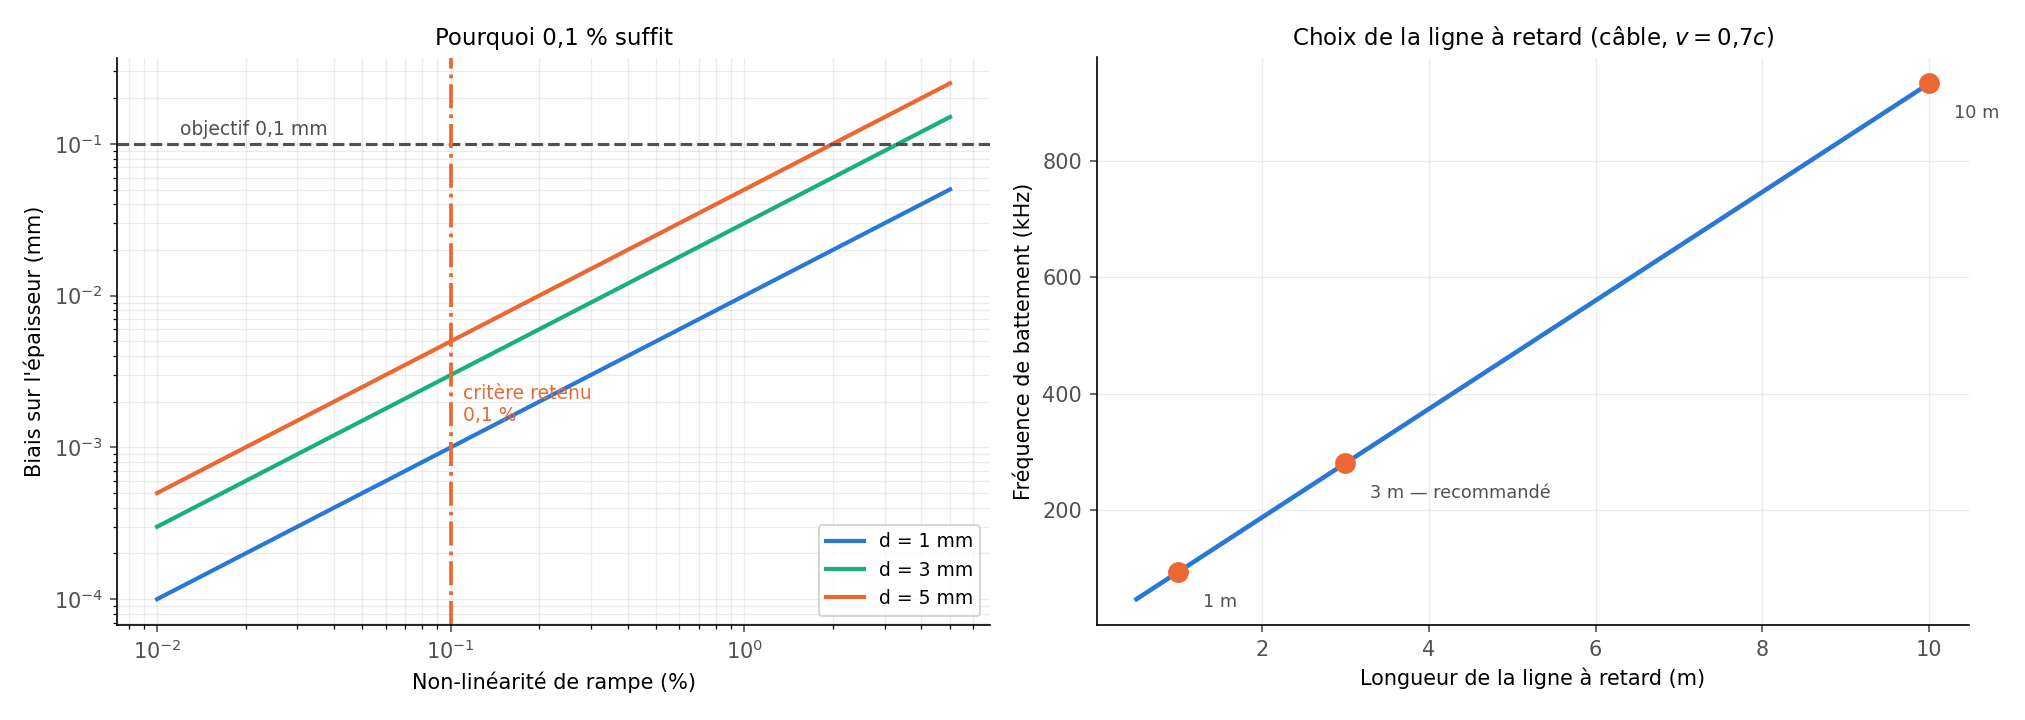
\includegraphics[width=\textwidth]{fig_p1_critere.png}
\end{center}

\begin{table}[H]
\centering
\begin{tabular}{lccc}
\toprule
Non-linéarité & $d = 1$~mm & $3$~mm & $5$~mm \\
\midrule
$1\,\%$ & $0{,}010$~mm & $0{,}030$~mm & $0{,}050$~mm \\
$\mathbf{0{,}1\,\%}$ & $0{,}001$~mm & $0{,}003$~mm & $\mathbf{0{,}005}$~mm \\
$0{,}01\,\%$ & $0{,}0001$~mm & $0{,}0003$~mm & $0{,}0005$~mm \\
\bottomrule
\end{tabular}
\end{table}

À $0{,}1\,\%$, le biais introduit vaut $0{,}005$~mm sur une couche de $5$~mm,
soit vingt fois moins que l'objectif de $0{,}1$~mm. C'est confortable, et c'est
ce qu'atteint couramment une boucle asservie.

\subsection{Ce que la phase 1 ne fait pas}

Elle ne cherche ni la compacité, ni la vitesse de balayage, ni l'intégration
mécanique, ni la conformité réglementaire. Le montage sera encombrant, alimenté
par plusieurs blocs de laboratoire, et posé sur une table. C'est voulu.

%=======================================================================
\section{Principe : pourquoi ce montage, et pourquoi il est simple}
%=======================================================================

\subsection{Le principe en une phrase}

On émet un signal dont la fréquence monte linéairement, on le mélange avec
l'écho qui revient, et la \emph{différence} de fréquence obtenue est
proportionnelle à la distance de la cible. Un aller-retour de $150$~mm donne
$20$~kHz : une fréquence audible.

\begin{attention}
C'est le point qui rend cette phase abordable : bien que le signal émis soit à
$8$~GHz, \textbf{tout ce que l'on mesure est de l'audio}. Un ordinateur muni
d'une carte son convient. Aucun oscilloscope rapide, aucun analyseur de spectre
hyperfréquence n'est indispensable.
\end{attention}

\subsection{Pas besoin de démodulateur IQ}

Un radar de ce type est souvent décrit avec un démodulateur en quadrature, qui
livre deux voies dites I et Q. C'est nécessaire lorsqu'il faut distinguer une
cible en avant d'une cible en arrière. Ici, toutes les cibles sont à des
distances positives : \textbf{un simple mélangeur suffit}, et la phase de la
réflexion --- dont nous avons besoin --- est intégralement préservée dans le
signal audio. Cela économise le composant le plus cher et le plus difficile à
trouver au-dessus de $6$~GHz.

\subsection{Architecture}

\begin{center}
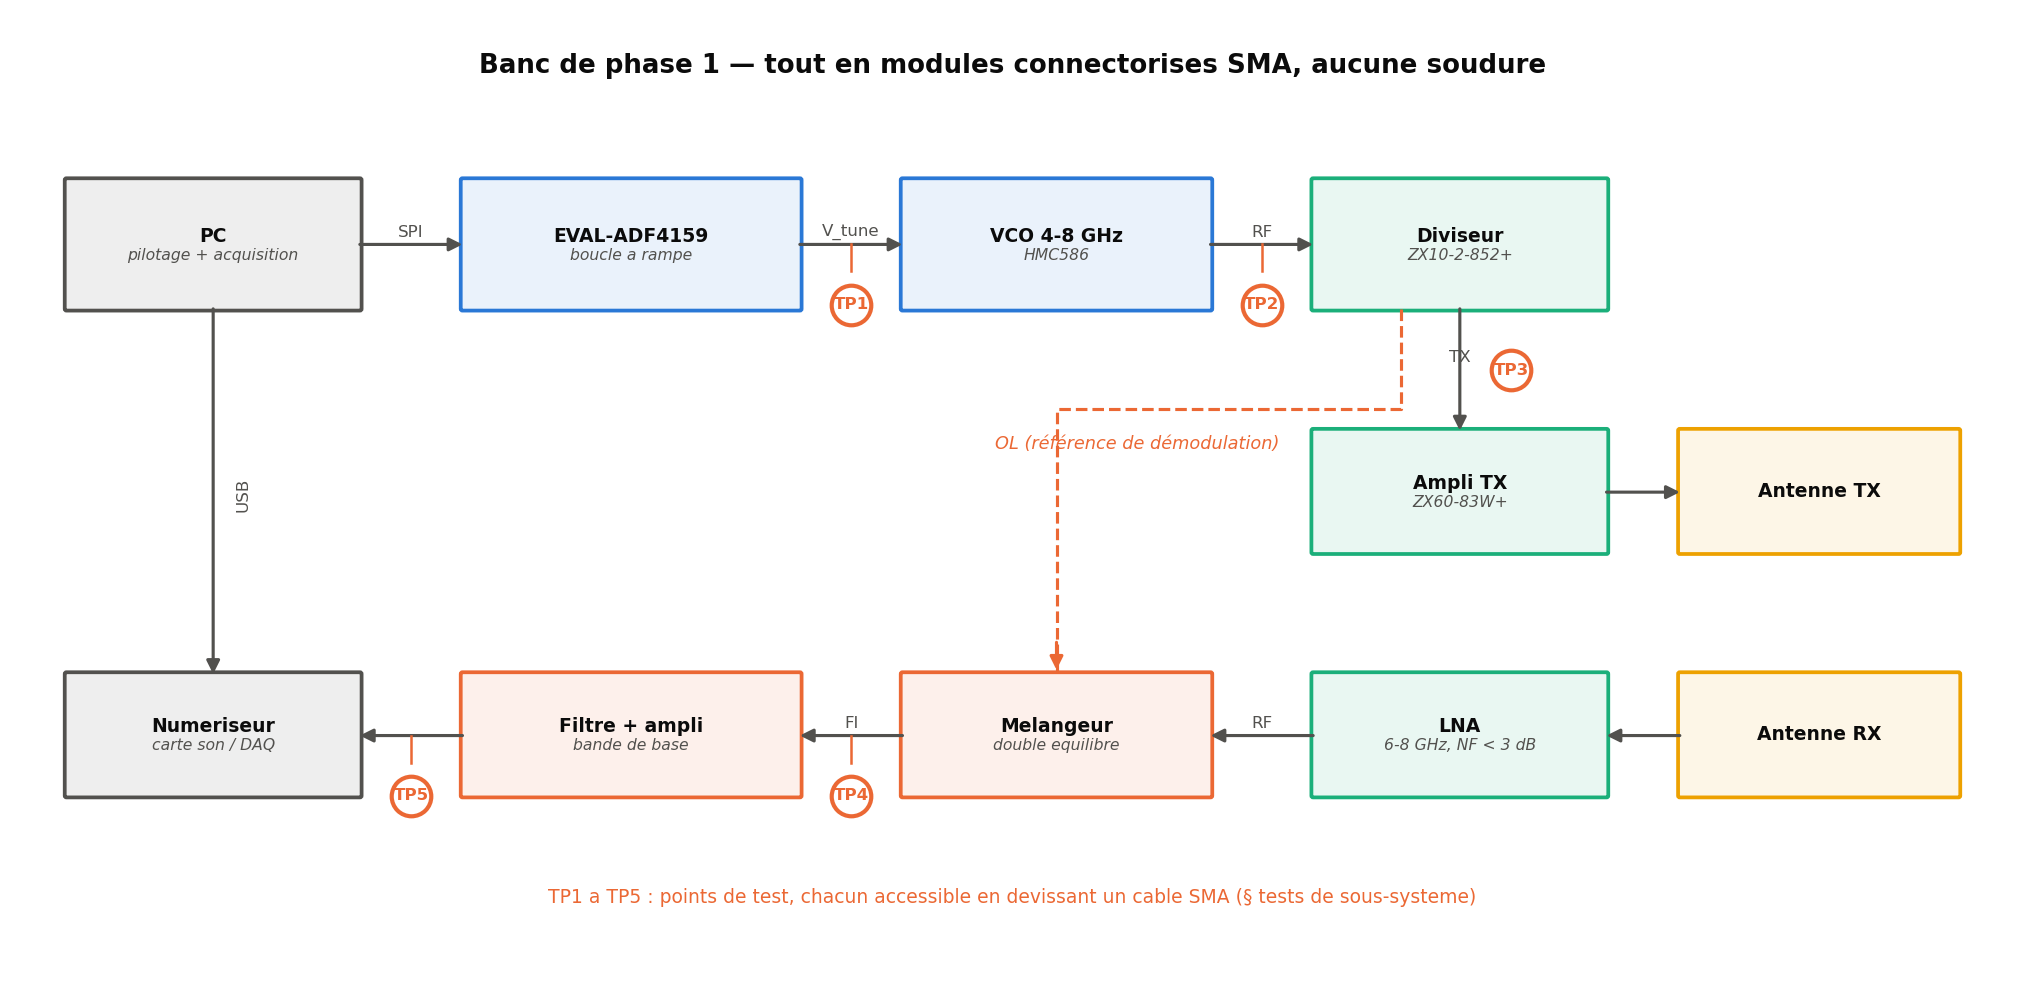
\includegraphics[width=\textwidth]{fig_p1_banc.png}
\end{center}

Le signal parcourt le chemin suivant. La \textbf{boucle à rampe} commande la
tension de réglage d'un \textbf{oscillateur} qui produit le balayage
$6$--$8$~GHz. Un \textbf{diviseur} en prélève une part qui servira de
référence ; le reste est amplifié et émis. L'écho reçu est amplifié par un
\textbf{amplificateur faible bruit} puis \textbf{mélangé} à la référence. Il en
sort un signal audio, filtré puis numérisé.

Les repères TP1 à TP5 sont des points de test : chacun s'obtient en dévissant
un câble SMA et en y branchant l'instrument de mesure.

%=======================================================================
\section{Nomenclature}
%=======================================================================

\begin{attention}
Les références ci-dessous sont des \emph{candidats}, cohérents avec le besoin au
moment de la rédaction. Les catalogues évoluent, et certaines cartes
d'évaluation sont fabriquées en petites séries. \textbf{L'étape~0 du projet est
de vérifier disponibilité, référence exacte de commande et prix} sur
\texttt{mouser.fr} avant tout achat. Ne commandez jamais un composant sans avoir
ouvert sa fiche technique et vérifié sa plage de fréquence.
\end{attention}

\begin{longtable}{>{\raggedright\arraybackslash}p{2.6cm}%
                  >{\raggedright\arraybackslash}p{5.4cm}%
                  >{\raggedright\arraybackslash}p{4.0cm}c}
\toprule
Fonction & Exigence & Candidat & Ordre de prix \\
\midrule
\endfirsthead
\toprule
Fonction & Exigence & Candidat & Ordre de prix \\
\midrule
\endhead
Boucle à rampe & synthétiseur fractionnaire jusqu'à $13$~GHz, générateur de
  rampe matériel & \textbf{EVAL-ADF4159} (version à VCO externe) & $300$--$500$~\texteuro \\[1mm]
Oscillateur & couvre $6{,}0$--$8{,}0$~GHz, sortie SMA, bruit de phase
  $< -95$~dBc/Hz à $100$~kHz & carte d'évaluation \textbf{HMC586LC4B}
  ($4$--$8$~GHz) & $200$--$400$~\texteuro \\[1mm]
Diviseur & $2$ voies, $0{,}5$--$8{,}5$~GHz, SMA & \textbf{ZX10-2-852+}
  (Mini-Circuits) & $60$--$100$~\texteuro \\[1mm]
Amplificateur d'émission & couvre $6$--$8$~GHz, gain $\sim 15$~dB, SMA
  & \textbf{ZX60-83W+} ($50$~MHz--$8$~GHz) & $100$--$150$~\texteuro \\[1mm]
Amplificateur faible bruit & couvre $6$--$8$~GHz, facteur de bruit $< 3$~dB
  & \emph{à choisir dans la même famille} & $100$--$200$~\texteuro \\[1mm]
Mélangeur & double équilibré, RF et OL couvrant $6$--$8$~GHz, FI continue à
  $1$~MHz & \emph{connectorisé SMA, niveau OL $+7$ à $+13$~dBm}
  & $100$--$200$~\texteuro \\[1mm]
Bande de base & filtre passe-bas $\sim 100$~kHz + amplificateur à gain réglable
  & module audio ou carte à monter & $50$--$150$~\texteuro \\[1mm]
Numériseur & $\ge 500$~kSa/s, $16$~bits, entrée différentielle
  & interface audio ou carte d'acquisition & $150$--$400$~\texteuro \\[1mm]
Antennes ($\times 2$) & couvrent $6$--$8$~GHz, faible encombrement
  & cornet ou antenne UWB à connecteur SMA & $100$--$300$~\texteuro \\[1mm]
Ligne à retard & $3$~m de câble coaxial faible perte, SMA
  & \emph{indispensable au test de linéarité} & $50$--$100$~\texteuro \\[1mm]
Câbles et accessoires & câbles SMA courts, adaptateurs, charges $50\,\Omega$,
  atténuateurs $3$ et $10$~dB & & $200$--$400$~\texteuro \\[1mm]
Alimentations & $2$ à $3$ voies de laboratoire, $0$--$15$~V, limitation en
  courant & & $200$--$400$~\texteuro \\[1mm]
Clé dynamométrique SMA & $0{,}5$~N$\cdot$m & & $30$--$60$~\texteuro \\
\midrule
\multicolumn{3}{l}{\textbf{Total indicatif}} & $\mathbf{1{,}6}$--$\mathbf{3{,}5}$~\textbf{k\texteuro} \\
\bottomrule
\end{longtable}

\subsection{Instruments de mesure}

\begin{table}[H]
\centering
\begin{tabular}{>{\raggedright\arraybackslash}p{4.6cm}%
                >{\raggedright\arraybackslash}p{9.4cm}}
\toprule
Instrument & Nécessité \\
\midrule
Multimètre & \textbf{indispensable} --- vérification des alimentations \\
Carte son ou acquisition & \textbf{indispensable} --- c'est l'instrument
  principal, le signal utile étant audio \\
LiteVNA (déjà possédé) & \textbf{très utile} jusqu'à $6{,}3$~GHz : vérification
  des câbles, du diviseur, des antennes, et référence de comparaison pour Q2 \\
Analyseur de spectre à $8$~GHz & \emph{souhaitable, non indispensable} ---
  le test de linéarité (§\ref{sec:testA}) s'en passe entièrement. À emprunter
  ou louer pour une journée si possible \\
\bottomrule
\end{tabular}
\end{table}

\begin{attention}
Le LiteVNA s'arrête à $6{,}3$~GHz et ne peut donc pas observer directement le
haut de la rampe. Ce n'est pas gênant : le test décisif convertit le balayage
en un signal audio, et se mesure sans aucun instrument hyperfréquence.
\end{attention}

%=======================================================================
\section{Sous-système A --- la source de rampe}
\label{sec:testA}
%=======================================================================

C'est le c\oe ur du projet et le seul véritable risque. Consacrez-lui la moitié
du temps.

\subsection{Rôle}

Produire un signal dont la fréquence monte de $6{,}0$ à $8{,}0$~GHz en
$100\,\mu$s, de façon aussi linéaire que possible, et recommencer $5\,000$ fois
par seconde.

\subsection{Pourquoi il faut une boucle asservie}

Un oscillateur commandé en tension possède une caractéristique
tension--fréquence \emph{fortement courbe} : appliquer une rampe de tension
donne une rampe de fréquence tordue, avec plusieurs pour-cent d'erreur. Les
réalisations amateur procèdent ainsi et se contentent de $100$~MHz d'excursion,
où la courbure reste tolérable. Sur $2$~GHz, c'est impossible.

La boucle à verrouillage de phase résout cela en \emph{asservissant} la
fréquence : elle la compare en permanence à une référence à quartz et corrige.
La linéarité ne dépend plus de l'oscillateur mais de la référence, stable à
quelques parties par million.

\subsection{Documentation à rassembler}

\begin{enumerate}[nosep]
\item La fiche technique de l'ADF4159 --- comprendre les registres de rampe
      (déviation, pas, durée).
\item Le guide utilisateur de la carte d'évaluation --- brochage,
      alimentations, connecteur de programmation.
\item Le logiciel \textbf{ADIsimPLL} du fabricant, gratuit. Il calcule le filtre
      de boucle et \emph{simule la rampe}.
\item La fiche technique du VCO --- plage de fréquence, sensibilité de réglage
      (MHz/V), plage de tension admissible.
\end{enumerate}

\subsection{Installation}

\begin{enumerate}
\item Alimentez la carte PLL seule, sans le VCO. Vérifiez chaque tension au
      multimètre.
\item Installez le logiciel de contrôle. Vérifiez la communication : un
      registre lu doit renvoyer ce qui y a été écrit.
\item \textbf{Concevez le filtre de boucle avec ADIsimPLL}, en saisissant la
      sensibilité réelle du VCO. Le logiciel fournit les valeurs des composants.
      C'est la seule étape qui demande de la méthode ; le logiciel fait le
      calcul.
\item Connectez le VCO. Vérifiez d'abord qu'il oscille en lui appliquant une
      tension de réglage fixe.
\end{enumerate}

\subsection{Test A1 --- le balayage existe-t-il ?}

\textbf{Montage :} sortie du VCO (TP2) vers un analyseur de spectre, en mode
mémoire de maximum. Si vous n'avez pas d'analyseur, passez directement au test
A2, qui est plus important.

\textbf{Attendu :} un plateau plat entre $6{,}0$ et $8{,}0$~GHz.

\begin{center}
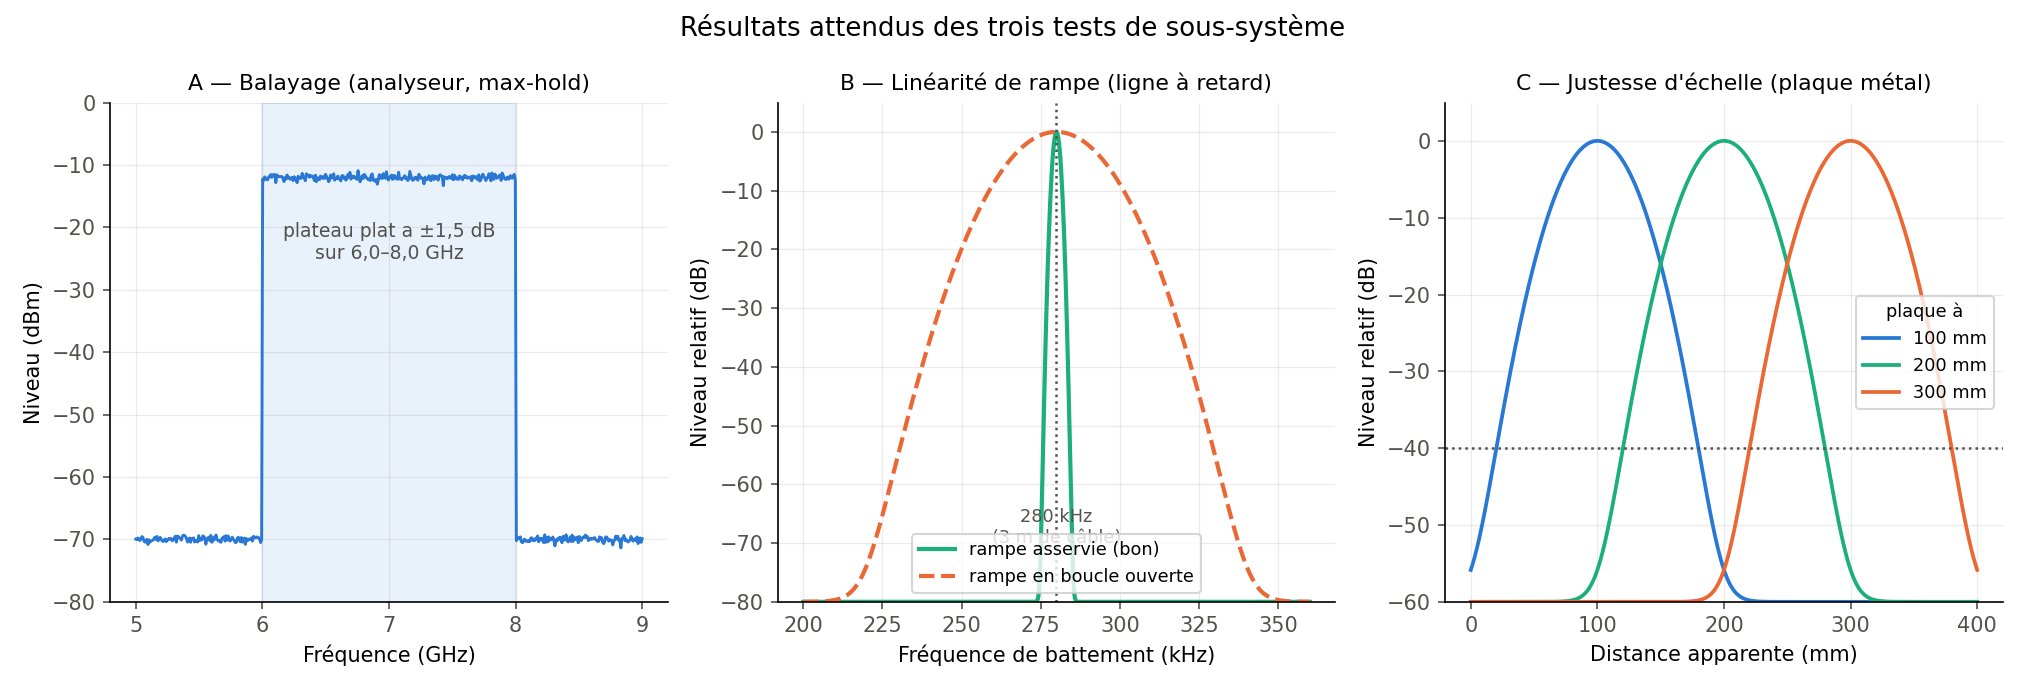
\includegraphics[width=\textwidth]{fig_p1_tests.png}
\end{center}

\begin{critere}
Plateau présent sur toute la plage, plat à $\pm 3$~dB, sans trou ni raie
parasite plus de $20$~dB au-dessus du plateau.
\end{critere}

\subsection{Test A2 --- la linéarité, sans instrument hyperfréquence}

C'est \textbf{le test décisif de toute la phase 1}. Son élégance tient à ce
qu'il n'exige rien d'autre que le montage lui-même.

\textbf{Principe.} On envoie la rampe dans un long câble et on mélange la sortie
du câble avec la rampe d'origine. Le câble introduit un retard connu, donc une
fréquence de battement connue. \emph{Si la rampe est parfaitement linéaire, ce
battement est une raie pure.} Toute non-linéarité l'élargit. La largeur de la
raie mesure donc directement la linéarité --- et cette raie est à $280$~kHz,
c'est-à-dire dans la bande d'une carte son.

\textbf{Montage :}
\begin{enumerate}[nosep]
\item Sortie VCO $\to$ diviseur.
\item Voie 1 du diviseur $\to$ \textbf{3~m de câble} $\to$ entrée RF du
      mélangeur.
\item Voie 2 du diviseur $\to$ entrée OL du mélangeur.
\item Sortie FI du mélangeur $\to$ filtre $\to$ numériseur.
\end{enumerate}

Aucune antenne, aucun amplificateur : uniquement le diviseur, le câble et le
mélangeur.

\textbf{Traitement :} enregistrez $100$ rampes, appliquez à chacune une
transformée de Fourier, et mesurez la largeur de la raie à $-6$~dB.

\begin{critere}
La raie de battement se situe à $280 \pm 10$~kHz et sa largeur à $-6$~dB est
inférieure à $\mathbf{3}$~\textbf{kHz}, soit $1\,\%$ de sa fréquence.\\[1mm]
\emph{Justification :} pour un retard fixe, l'élargissement relatif de la raie
est égal à la non-linéarité relative de la rampe. Une raie large de $1\,\%$
correspond donc à $1\,\%$ de non-linéarité --- déjà acceptable pour
$0{,}03$~mm de biais. Viser $0{,}3$~kHz ($0{,}1\,\%$) pour la marge complète.
\end{critere}

Si la raie est large de plusieurs dizaines de kilohertz, la boucle n'asservit
pas correctement : reprenez le filtre de boucle dans ADIsimPLL, en réduisant la
bande passante de boucle.

%=======================================================================
\section{Sous-système B --- la voie d'émission}
%=======================================================================

\textbf{Rôle.} Prélever une part du signal pour la référence, amplifier le
reste et l'émettre.

\textbf{Test B1 --- le diviseur.} Mesurable au LiteVNA jusqu'à $6{,}3$~GHz :
$-3{,}5$~dB environ sur chaque voie, isolation meilleure que $18$~dB entre
voies. Un écart franc signale un connecteur mal serré.

\textbf{Test B2 --- l'amplificateur.} Alimentez-le, injectez un signal connu,
mesurez le gain. Vérifiez le courant consommé : conforme à la fiche technique à
$\pm 20\,\%$.

\begin{attention}
Ne branchez \textbf{jamais} un amplificateur sans charge à sa sortie : une
sortie ouverte peut le détruire. Une charge $50\,\Omega$ vissée est la position
de repos.
\end{attention}

%=======================================================================
\section{Sous-système C --- la voie de réception}
%=======================================================================

\textbf{Rôle.} Amplifier l'écho, puis le mélanger à la référence.

\textbf{Test C1 --- l'amplificateur faible bruit.} Même procédure que B2.

\textbf{Test C2 --- le mélangeur.} Injectez deux signaux de fréquences voisines
sur RF et OL, vérifiez que la sortie FI porte bien leur différence.

\begin{attention}
Un mélangeur exige un niveau de référence \emph{précis} sur son entrée OL
(typiquement $+7$ à $+13$~dBm). Trop faible, il ne fonctionne pas ; trop fort,
il sature. C'est le rôle des atténuateurs de la nomenclature : ajustez le
niveau avec un atténuateur de $3$ ou $10$~dB plutôt qu'en modifiant le montage.
\end{attention}

%=======================================================================
\section{Sous-système D --- bande de base et numérisation}
%=======================================================================

\textbf{Rôle.} Filtrer et amplifier le signal audio, puis le numériser en
synchronisme avec la rampe.

\textbf{La synchronisation est le point délicat.} Chaque enregistrement doit
commencer au début d'une rampe, sinon les rampes successives ne peuvent pas être
moyennées. La carte PLL fournit un signal indiquant le début de rampe :
utilisez-le comme déclenchement du numériseur.

\textbf{Test D1.} Injectez une sinusoïde connue de $20$~kHz à l'entrée. Vérifiez
que la transformée de Fourier la restitue à la bonne fréquence et à la bonne
amplitude, et que le plancher de bruit descend de $3$~dB chaque fois que l'on
double le nombre de moyennes --- preuve que le moyennage est cohérent.

%=======================================================================
\section{Intégration progressive}
%=======================================================================

N'assemblez jamais tout d'un coup. À chaque étape, un seul élément nouveau.

\begin{table}[H]
\centering
\begin{tabular}{clp{7.4cm}}
\toprule
Étape & Ajout & Vérification \\
\midrule
1 & PLL + VCO & test A1 et A2 \\
2 & + diviseur, câble de $3$~m & test A2 complet, raie à $280$~kHz \\
3 & + bande de base et numériseur & test D1, moyennage cohérent \\
4 & + amplificateur d'émission & niveau à TP3 conforme \\
5 & + LNA & gain total mesuré \\
6 & + antennes & premier écho réel \\
\bottomrule
\end{tabular}
\end{table}

%=======================================================================
\section{Plan de test système}
%=======================================================================

\subsection{Test S1 --- justesse de l'échelle des distances}

\textbf{Montage :} antennes face à une plaque métallique, à $100$, $200$ puis
$300$~mm mesurés au réglet.

\textbf{Attendu :} un pic unique dont la position croît linéairement avec la
distance réelle (panneau C de la figure des tests).

\begin{critere}
Écart entre distance mesurée et distance réelle inférieur à $2\,\%$, et
\emph{constant} en pourcentage. Un écart constant en pourcentage est une erreur
de pente de rampe, corrigible par le calcul ; un écart variable révèle une
non-linéarité résiduelle.
\end{critere}

\subsection{Test S2 --- calibration}

Appliquez la même procédure que celle déjà en service sur le LiteVNA
(\texttt{calibration.py}) : mesurez un court-circuit, un circuit ouvert et
une charge au plan de référence, résolvez les trois termes d'erreur, puis
vérifiez que la charge, une fois corrigée, tombe sous le plancher.

\begin{critere}
Après correction, la réflexion résiduelle de la charge est inférieure à
$-30$~dB.
\end{critere}

\subsection{Test S3 --- comparaison au LiteVNA (le test final)}

C'est celui qui répond à Q2. Choisissez une cible stable : d'abord une plaque
métallique à $150$~mm, puis une lame de \textbf{PMMA} (plexiglas,
$\eps = 2{,}6$) posée sur un bloc de polystyrène expansé, rien derrière. Une
lame libre dans l'air a deux interfaces de coefficients égaux au signe près :
ses deux échos ont donc la même amplitude, ce qui en fait la cible la plus
facile qui soit. Une épaisseur de $50$~mm convient ; mesurez-la au pied à
coulisse en cinq points, et demandez du PMMA \emph{coulé}, dont la tolérance
d'épaisseur est bien meilleure que celle de l'extrudé.

\begin{enumerate}[nosep]
\item Mesurez $\Gamma(f)$ avec le LiteVNA calibré, sur $6{,}0$--$6{,}3$~GHz
      (le haut de sa plage).
\item Mesurez la même cible avec le banc FMCW, calibré, sur la même
      sous-bande.
\item Superposez amplitude et phase.
\end{enumerate}

\begin{critere}
Sur la sous-bande commune $6{,}0$--$6{,}3$~GHz, l'écart entre les deux mesures
est inférieur à $\mathbf{1}$~\textbf{dB} en amplitude et $\mathbf{5^\circ}$ en
phase, après retrait d'un retard et d'un gain complexe constants.
\end{critere}

\begin{attention}
Ce test est le plus important du guide. Il ne vérifie pas une performance : il
vérifie que le banc mesure \emph{la même grandeur physique} qu'un instrument de
métrologie déjà calibré. Tant qu'il n'est pas passé, aucun résultat du banc
n'est exploitable.
\end{attention}

%=======================================================================
\section{Décision de fin de phase}
%=======================================================================

\begin{table}[H]
\centering
\begin{tabular}{>{\raggedright\arraybackslash}p{5.0cm}%
                >{\raggedright\arraybackslash}p{9.4cm}}
\toprule
Résultat & Conclusion \\
\midrule
A2 $< 0{,}3$~kHz, S3 conforme & \textbf{Risque levé.} Engager la phase 2
  (prototype intégré) \\[1mm]
A2 entre $0{,}3$ et $3$~kHz, S3 conforme & \textbf{Risque levé avec réserve.}
  Utilisable ; améliorer la boucle en phase 2 \\[1mm]
A2 $> 3$~kHz malgré plusieurs filtres de boucle & \textbf{Reconsidérer.}
  Essayer une excursion réduite ($6$--$7$~GHz), ou une architecture à rampe
  numérique \\[1mm]
S3 non conforme, A2 conforme & Le problème est dans la réception ou la
  calibration, non dans la rampe. Reprendre les tests C et S2 \\
\bottomrule
\end{tabular}
\end{table}

\begin{attention}
Une phase 1 qui conclut « non » en trois mois et quelques milliers d'euros est
un \emph{succès} : elle évite une phase 2 d'un an. Le seul mauvais résultat est
un résultat ambigu, faute d'avoir suivi les critères chiffrés.
\end{attention}

%=======================================================================
\section{Pièges les plus fréquents}
%=======================================================================

\begin{enumerate}
\item \textbf{Confondre plage de l'oscillateur et excursion balayée.} Un VCO
      « $4$--$8$~GHz » ne garantit pas que la boucle balaie $2$~GHz d'un trait.
      C'est précisément ce que teste A2.
\item \textbf{Câble déplacé entre deux mesures.} Toute flexion change la phase
      et ruine la calibration. Fixez les câbles avec du ruban adhésif.
\item \textbf{Niveau OL incorrect.} Cause la plus fréquente d'un mélangeur qui
      « ne marche pas ».
\item \textbf{Absence de déclenchement.} Sans signal de début de rampe, le
      moyennage détruit le signal au lieu de l'améliorer. Symptôme : le niveau
      \emph{baisse} quand on moyenne.
\item \textbf{Antennes trop proches.} À moins de $80$~mm, l'écho d'antenne et
      celui de la cible se confondent. Travaillez d'abord à $150$--$300$~mm ;
      la mesure à $20$~mm relève de la phase 2.
\item \textbf{Vouloir tout mesurer d'un coup.} Le tableau d'intégration
      progressive existe pour cela : un seul élément nouveau à la fois.
\end{enumerate}


\end{document}
